\documentclass[11pt,a4paper]{report}
\usepackage[utf8]{inputenc}

\PassOptionsToPackage{obeyspaces}{url}

\usepackage[dvipsnames]{xcolor}
\usepackage{tikz}
\usetikzlibrary{decorations.pathreplacing}
\usepackage{graphicx}

\usepackage{biblatex}

\usepackage{enumitem}
\usepackage{subcaption}
\usepackage{listings}
\usepackage{multicol}

\usepackage{xurl}
\usepackage{hyperref}

\addbibresource{content/references/books.bib}
\addbibresource{content/references/links.bib}
\addbibresource{content/references/papers.bib}

\lstset{basicstyle=\ttfamily\footnotesize,
	keepspaces=true,
	backgroundcolor=\color{lightgray},
	showstringspaces=false,
	upquote=true,
	breaklines=true,
	numbers=left,
}

\renewcommand*\Itemautorefname{technique}

\hypersetup{
	colorlinks=true,
	urlcolor = NavyBlue,
	citecolor = Maroon,
	linkcolor = Violet,
}

\begin{document}

\begin{titlepage}
	\begin{center}
		\textsc{\LARGE Master thesis\\Computing Science: Cyber Security}\\[1.5cm]
		\includegraphics[height=100pt]{resources/images/logo}

		\vspace{0.4cm}
		\textsc{\Large Radboud University}\\[1cm]
		\hrule
		\vspace{0.4cm}
		\textbf{\huge Detecting Capabilities in Malware Binaries by Searching for Function Calls}\\[0.4cm]
		\hrule
		\vspace{2cm}

		\begin{minipage}[t]{0.45\textwidth}
			\begin{flushleft}
				\large
				\textit{Author:}\\ Joren Vrancken\\ s4593847
			\end{flushleft}
		\end{minipage}
		\begin{minipage}[t]{0.45\textwidth}
			\begin{flushright}
				\large \textit{Supervisor \& First Assessor:}\\ dr. ir. Erik Poll\\ \href{mailto:erikpoll@cs.ru.nl}{\texttt{erikpoll@cs.ru.nl}}\\[1.3cm]
				\textit{Second assessor:}\\ dr. Freek Verbeek\\ \href{mailto:freek@vt.edu}{\texttt{freek@vt.edu}}
			\end{flushright}
		\end{minipage}
	\vfill
	{\large \today}
	\end{center}
\end{titlepage}

\section*{Acknowledgments}\label{chapter:acknowledgments}
I would like to sincerely thank everybody that helped me write this thesis. In particular, I would like to thank Erik Poll. His guidance and thoughtful questions about my approach made me think deeper about the research. It was a joy and great learning experience to work with him. Multiple people have provided feedback and guidance throughout the research and proofread the thesis. My wholehearted thanks to you all. This thesis has become much better because all of you.

\thispagestyle{empty}

\begin{abstract}\label{chapter:abstract}
    Incidents like the ransomware attack on the Colonial Pipeline in 2021 \cite{pipeline-attack} show that malware is a growing threat with real-world implications. To combat this growing threat, there is an ever-growing need for (automated) malware analysis tools.

    \medskip

    Meaningful actions by applications (including malware) require interaction with the operating system. Operating systems facilitate this by providing an API. Malicious activity is often implemented via calls to this API. Such calls can be seen as an indicator of the malicious activity.

    As most malware is written for Windows \cite{windows-malware}, we focus on Windows and the Windows API.

    \medskip

    In this thesis, we present a method to detect malware capabilities by searching for specific function calls with specific arguments. This method consists of two steps: (1) describing the function calls that are used to implement a capability as patterns, including the arguments that are passed to such functions, and (2) searching for these patterns in malware binaries.

    For the first step, we provide patterns to describe function calls: \emph{Call Signatures}. For the second step, we developed an IDA Pro plugin, called Call Signatures Plugin (\emph{CSP}), that uses Call Signatures to search for function calls in a binary. This plugin is available at \url{https://github.com/joren485/CallSignaturesPlugin}.

    \medskip

    To showcase the effectiveness of detecting capabilities with Call Signatures and CSP, we perform an experiment where we use them to detect a capability that is commonly implemented by malware: \emph{persistence}. Persistence is the class of techniques that malware use to maintain access to a victim system after an initial infection. We provide an overview of common persistence techniques and the function calls that are required to implement these techniques. We express these function calls, including their arguments, as Call Signatures and then use CSP to search for these techniques in a dataset of real-world malware samples.

    The outcome of this experiment shows that function calls can be an effective indicator for detecting malware capabilities. We also show that Call Signatures and CSP perform well compared to existing tooling.
\end{abstract}


\tableofcontents

\chapter{Introduction}\label{chapter:introduction}
Malware is software that is made with malicious intent. Its goal is to disrupt or damage computer systems, users, or networks \cite{microsoft-malware} \cite{practical-malware-analysis}. Criminals have started using malware for monetary gain. For example, by stealing banking and credit card information \cite{banking-malware} or by disrupting systems until a ransom has been paid \cite{ransomware}. The global intelligence community has also embraced malware to stealthily infiltrate the systems of adversaries \cite{perfect_weapon}. Their goals are not monetary\footnote{A notable exception to this is North Korea \cite{north-korea-chainalysis}.}, but rather stealing sensitive information, espionage, or disruption of vital sectors \cite{countdown-to-zero-day} \cite{sandworm}.

The increased use of malware has increased the need for defense against and analysis of malware. Today many companies provide commercial antivirus suites that will scan consumer systems for known malware and malware behavior (e.g. Norton\footnote{\tiny \url{https://us.norton.com/}}, Kaspersky\footnote{\tiny \url{https://www.kaspersky.com/}}, and F-Secure\footnote{\tiny \url{https://www.f-secure.com/}}). Other companies focus on helping larger organizations protect themselves and perform incident response once a breach has been detected (e.g. Mandiant\footnote{\tiny \url{https://www.mandiant.com/}} and CrowdStrike\footnote{\tiny \url{https://www.crowdstrike.com/}}). This has created a digital arms race where malware authors will use evermore advanced techniques to evade detection and malware analysts will use evermore advanced techniques to detect malware.

Malware analysis is the process of studying malware samples to try to determine their functionality, origin, and targets \cite{practical-malware-analysis}. It plays an important role in the defense against malware. Malware analysis helps understand known malware and discover unknown malware.

According to the AV-test institute, about four hundred fifty thousand new malware samples are found every day \cite{av-test}. To process and analyze such a vast amount of data, we need tooling that automates malware analysis.

\medskip

In this thesis, we look at how to statically detect high-level functionality in malware binaries, by searching for patterns of function calls. Because API function calls are crucial to applications for any meaningful interaction with the operating system, we decided to detect high-level functionality using function calls (with specific arguments) as an indicator. Calls to API functions are harder to obfuscate than other parts of malware, as API functions are pre-defined by the operating system.

We define high-level functionality (i.e. capabilities) as \emph{what} a malware sample is capable of (e.g. lateral movement, privilege escalation, and persistence). In contrast to low-level functionality, which describes \emph{how} a malware sample implements the high-level functionality (e.g. implementing disk encryption with AES encryption). We choose to focus on high-level functionality as it is more helpful to a malware analyst to know what a sample is capable of. For example, it is generally more interesting to know that a sample encrypts files than that a sample uses AES encryption.

As most malware is written for Windows \cite{windows-malware}, we will focus on Windows binaries. Almost all newly sold Windows computers run a 64-bit version of Windows \cite{64-bit-malware}. However, as 64-bit Windows provides backward compatibility for 32-bit executables \cite{wow64}, most malware is still written for 32-bit \cite{64-bit-malware}, as it allows a single executable to infect both 32-bit and 64-bit machines. Therefore, we will focus specifically on malware made for 32-bit Windows.

\medskip

Before we discuss the research itself, we first go over related research (\autoref{chapter:related work}) and background information. In \autoref{chapter:background x86 windows}, we discuss background information on x86, function calls and Windows, and in \autoref{chapter:background malware} we discuss malware and malware analysis.

\medskip

We split the detection of high-level functionality into two steps:
\begin{enumerate}
    \item Defining patterns for the function calls that are commonly used to implement the functionality. In \autoref{chapter:call signatures}, we introduce such patterns: \emph{Call Signatures}.

    \item Searching for function calls that match these patterns in binaries. In \autoref{chapter:plugin}, we develop an IDA Pro plugin, called \emph{CSP}, that uses Call Signatures to search for function calls in binaries. We choose to develop a plugin for IDA Pro, because IDA Pro is the most popular reverse engineering toolkit \cite{ida_guide}.
\end{enumerate}

\medskip

We test and showcase the usage of Call Signatures and CSP by using them to detect specific high-level functionality in real-world malware samples.

The high-level functionality we will focus on is persistence, the capability that describes how malware maintains access to an infected victim. We choose to focus on persistence as it is commonly implemented by malware \cite{practical-malware-analysis}.

First, we analyze which techniques are commonly used by malware to achieve persistence (in \autoref{chapter:persistence techniques}). Second, in \autoref{chapter:call signatures for persistence techniques}, we analyze the function calls used to implement these techniques and write Call Signatures to describe them.

In \autoref{chapter:experiments}, we create datasets of malware samples that implement four different persistence techniques and run CSP on each dataset to see how well it can detect the persistence techniques. We also run another static analysis tool (Capa by Mandiant) on the datasets, to see how Call Signatures and CSP compare to existing tooling.

\medskip

We conclude by looking at interesting ideas to expand upon this research (\autoref{chapter:future work}) and with a discussion (\autoref{chapter:conclusions}).

\chapter{Related Work}\label{chapter:related work}
Analyzing the functionality of binaries (without running them) is an active field of research with multiple approaches. An important driver for analyzing the functionality of binaries is malware analysis, as malware authors are actively trying to circumvent existing analysis techniques.

\medskip

A common way to detect and classify malware functionality is to look for code reuse between a potential malware sample and known malware samples. Because the source code of malware binaries is generally not available, assessing code reuse requires a similarity analysis of the binaries.

Haq and Caballero survey research on the similarity of binary code \cite{similarity-binary-code}. The research they survey focuses on semantic similarity, considering two binaries equivalent if they provide the same exact functionality. For example, a call graph-based approach by Lee et al. \cite{binary-similarity-call-graph} and BinSim by Ming et al. \cite{binsim} uses symbolic execution to analyze the logic in a binary. As there are countless ways to implement functionality, checking for semantic similarity is a complex process. To make matters worse, malware often implements obfuscation techniques to hide its functionality.

Other code reuse research looks at binaries as sequences of bytes. The general hypothesis being that similar source code results in similar compiled byte sequences. A popular technique is fuzzy-hashing: computing multiple hashes on sections of two inputs to find similar sections in the inputs \cite{piecewise-hashing}. For example, the research by Naik et al. \cite{fuzzy-import-hashing} and Namanya et al. \cite{fuzzy-hashing-combinational}. In \autoref{appendix:binlex experiment} we see a weakness of such approaches: similar code can be compiled into vastly different binary code.

\medskip

Machine learning is also being used to detect malicious functionality. As executable binaries are very complex data structures, either the neural network that is used to analyze the binaries needs to understand the general structure of such binaries or, pre-processing needs to take place to extract useful features to use in a neural network. For example, Raff et al. \cite{eat-exe} and Massarelli et al. \cite{safe} opt for the former approach and Xu et al. \cite{gemini} for the latter.

\medskip

Many reverse engineering tools implement a database of commonly inlined functions (e.g. standard library functions). The most well-known being F.L.I.R.T. (Fast Library Identification and Recognition Technology) in IDA Pro \cite{flirt}. Other examples are Function ID in Ghidra \cite{ghidra-fid} and Talos FIRST (Function Identification and Recover Signature Tool) \cite{talos-first}. The goal of these databases is to find known (uninteresting) functions. This tells malware analysts, for example, which functions to skip when they are reverse engineering a malware sample. They work by creating signatures of commonly inlined functions (often the first 32 bytes of the function). Functions in a binary can be checked against these signatures.

\medskip

The methodology we present in \autoref{chapter:call signatures} uses patterns to search for elements of interest (i.e. function calls) in a binary. In recent years there have been similar approaches. For example, FindFunc\footnote{\tiny \url{https://github.com/FelixBer/FindFunc}}, a tool that allows for advanced searching of byte patterns in binaries.

Pattern matching is also used in source code analysis. For example, software that searches for common vulnerabilities in code (e.g. Semgrep\footnote{\tiny \url{https://semgrep.dev/}}, CodeQL\footnote{\tiny \url{https://codeql.github.com/}}, and Weggli\footnote{\tiny \url{https://github.com/googleprojectzero/weggli/}}) define patterns that describe these vulnerabilities to search for in the code.

\medskip

Most similar to our research is Capa by Mandiant\footnote{\tiny \url{https://github.com/mandiant/capa}}. It identifies a broad spectrum of capabilities (e.g. cryptography, persistence, communication, and anti-analysis) in malware binaries. They define capabilities as rules of strings, byte sequences, and operating system API calls (similar to Yara signatures) that need to be present in functions. If all elements of a rule are present in a function, the sample is considered to have the capability that the rule defines. Unlike our research, their approach does not define a relation between the different elements that need to be present, which may cause false positives. We compare our work with Capa in \autoref{chapter:experiments}.

\chapter{Background on x86 \& Windows}\label{chapter:background x86 windows}
We will first go over the necessary background information. In \autoref{section:background x86}, we give general information on the CPU architecture that is used by Windows, x86. As this provides information on general concepts (registers, memory management, and assembly), it can be skipped by people that are familiar with these subjects. After that, we will discuss function calls and how they work in assembly, in \autoref{section:function calls}. Finally, we will discuss Windows. As Windows is a large, complex platform and operating system, we will focus on concepts that are used in this thesis: the Windows API, the Windows Registry, Windows Services, and Scheduled Tasks.

In the next chapter we will discuss malware (\autoref{chapter:background malware}).

\section{The x86 Architecture}\label{section:background x86}
CPUs perform operations by executing instructions. The model that describes these instructions is called an \emph{instruction set architecture}. x86, an instruction set architecture developed by Intel, is the most widely used instruction set architecture \cite{x86-dominance}.

An instruction indicates what operation the CPU should perform on data, stored in \emph{registers} (\autoref{section:registers}) and in the computers' memory.

An important feature of an instruction set architecture is the size of the registers and memory addresses. For example, a 32-bit architecture means that the registers and memory addresses consist of 32 bits and can store $2^{32}$ different values. The 32-bit variant of the x86 architecture is called IA-32 (Intel Architecture, 32-bit). However, most modern systems use the 64-bit variant, x86-64. x86-64 has full backward compatibility with IA-32, meaning that applications compiled for IA-32 can run on x86-64 (as long as the operating system also supports running IA-32 binaries).


\subsection{Registers}\label{section:registers}
Registers are small storage units that a CPU uses to store data during computations. Registers are implemented on the CPU itself, making data access significantly faster than accessing data stored in memory. There are two types of registers: general purpose registers and special purpose registers.

\subsubsection{General-purpose Registers}
General-purpose registers are used to store data or a memory address (i.e. a pointer) to data. x86 (specifically IA-32) has eight general-purpose registers, each having a traditional purpose. However, most can also be used for other purposes.

\begin{itemize}
    \item \texttt{eax} (extended\footnote{32-bit registers are called ``extended'' to distinguish them from their 16-bit counterpart. For example, the 32-bit \texttt{eax} register and the 16-bit \texttt{ax} register.} accumulator register): Used in arithmetic operations.
    \item \texttt{ebx} (extended base register): Used as a pointer to data stored in memory.
    \item \texttt{ecx} (extended counter register): Stores the counter in looping operations.
    \item \texttt{edx} (extended data register): Used in I/O operations.
    \item \texttt{esi} (extended source index): Stores the address of the input data in certain operations on strings.
    \item \texttt{edi} (extended destination index): Stores the address of the output data in certain operations on strings.
    \item \texttt{ebp} (extended base pointer): Stores the address of the base of the current stack frame.
    \item \texttt{esp} (extended base stack pointer): Stores the address to the top of the stack.
\end{itemize}

In IA-32 these registers are larger versions of the registers used in the 16-bit and 8-bit variants of x86. For backward compatibility, x86 allows access to the 16-bit and 8-bit registers as the lower half of the 32-bit registers. Similarly, the 32-bit registers can be accessed in x86-64. \autoref{table:registers} shows how these register sizes relate to each other, using the \texttt{eax} register as an example.

\begin{table}[ht]
    \centering
    \begin{tabular}{|l|llllllll|}
        \hline
        \textbf{64-bit} & \multicolumn{8}{c|}{\texttt{rax}} \\ \hline
        \textbf{32-bit} & & & & \multicolumn{1}{l|}{} & \multicolumn{4}{c|}{\texttt{eax}} \\ \hline
        \textbf{16-bit} & & & & & & \multicolumn{1}{l|}{} & \multicolumn{2}{c|}{\texttt{ax}} \\ \hline
        \textbf{8-bit} & & & & & & \multicolumn{1}{l|}{} & \multicolumn{1}{l|}{\texttt{ah}} & \texttt{al} \\ \hline
    \end{tabular}
    \caption{The relation between the different accumulator registers in variants of x86.}
    \label{table:registers}
\end{table}

\subsubsection{Special Purpose Registers}
Besides the general-purpose registers, x86 also has registers that store specific information about the program state and the CPU state. Two important registers with a specific purpose are:
\begin{itemize}
    \item \texttt{eflags} (extended flags): Stores the data of previous instructions (e.g. the result of a comparison of two values) and the processor state as booleans.
    \item \texttt{eip} (extended instruction pointer): Stores the address of the next instruction.
\end{itemize}


\subsection{The Stack}\label{section:stack}
A \emph{stack} is a data structure to store elements. We can add elements to the stack and take elements from the stack, with the restriction that the element that was added last is always the first element that is taken from the stack. This makes a stack a LIFO (last in, first out) data structure. A stack has two operations:
\begin{itemize}
   \item \textbf{Push}: Add a new element on top of the stack.

   \item \textbf{Pop}: Remove the top (i.e. the most recently added) element from the stack.
\end{itemize}

x86 uses a stack in memory to store the state of function calls, called the \emph{call stack}. Each time a function is called, a \emph{stack frame} is pushed to the call stack. A stack frame stores the arguments, return address, and local variables of a function. When a function returns, the stack frame is popped from the stack.

The call stack grows downwards. When an application starts, the stack pointer is set to some address. When data is pushed on the stack, the stack pointer is \emph{decreased}. Likewise, when data is popped from the stack, the stack pointer is \emph{increased}.

\autoref{fig:stack} illustrates what the stack would look like if a function \texttt{f0} has called another function \texttt{f1}. As we can see, the call frame of the callee is at the top of the stack, on top of the stack frame of the caller.

\begin{figure}[ht]
   \centering
   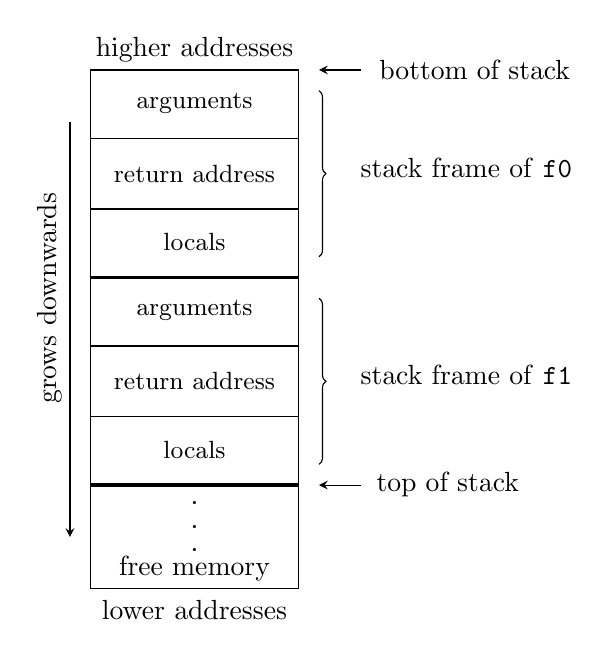
\begin{tikzpicture}[x=0.75pt,y=0.75pt,yscale=-1,xscale=1]

       % Arrow left of stack
       \draw (0,110) node[rotate=90] {grows downwards};
       \draw [-stealth] (10,25) -- (10,225) ;

       % Stack rectangle
       \draw (20,0) -- (120,0) -- (120,250) -- (20,250) -- cycle ;

       % Stack inside
       %% f0
       \draw (70,16) node {\small arguments};
       \draw (20,33) -- (120,33) ;
       \draw (70,50) node {\small return address};
       \draw (20,67) -- (120,67) ;
       \draw (70,83) node {\small locals};

       %% f1
       \draw [very thick] (20,100) -- (120,100) ;
       \draw (70,116) node {\small arguments};
       \draw (20,133) -- (120,133) ;
       \draw (70,150) node {\small return address};
       \draw (20,167) -- (120,167) ;
       \draw (70,183) node {\small locals};

       %% free memory
       \draw [very thick] (20,200) -- (120,200) ;
       \draw (70,220) node[rotate=90] {\large . . . };
       \draw (70,240) node {free memory};

       % Addresses
       \draw (70, -10) node {higher addresses};
       \draw (70, 260) node {lower addresses};

       %% Bottom of stack
       \draw [stealth-] (130,0) -- (150,0) ;
       \draw (205, 0) node {bottom of stack};

       %% Top of stack
       \draw [stealth-] (130,200) -- (150,200) ;
       \draw (192, 200) node {top of stack};

       %% Brace f0
       \draw [decorate, decoration={brace}] (130,10) -- (130,90) ;
       \draw (201,47) node {stack frame of \texttt{f0}};

       %% Brace f1
       \draw [decorate, decoration={brace}] (130,110) -- (130,190) ;
       \draw (201,147) node {stack frame of \texttt{f1}};
   \end{tikzpicture}
   \caption{The layout of the stack when \texttt{f0} has called \texttt{f1}.}
   \label{fig:stack}
\end{figure}

\medskip

Not all data of a program is stored on the stack. Larger and dynamically allocated data is stored in the \emph{heap}. Static and global variables are stored in a separate data segment.


\subsection{Assembly}\label{section:assembly}
Assembly is a low-level programming language in which, generally speaking, each statement corresponds to one instruction executed by the CPU. Assembly statements are compiled into byte sequences of machine code called \emph{opcodes}.

An assembly statement starts with the name of the instruction (the \emph{mnemonic}), followed by its operands (i.e. arguments). \autoref{listing:assembly example} shows an assembly statement where \texttt{mov} is the mnemonic and \texttt{eax} and \texttt{1} are the operands.

\begin{lstlisting}[caption={A single instruction moving the integer \texttt{1} into the register \texttt{eax}.}, label={listing:assembly example}, captionpos=b]
mov eax, 1
\end{lstlisting}

x86 assembly code is written in either Intel syntax (mostly used for Windows development) or AT\&T syntax (mostly used for Linux development). As we focus on Windows in this thesis, we will use the Intel syntax style.

In this section, we will discuss some basic instructions. There are, however, many more instructions used to efficiently perform operations on specific data types.

\subsubsection{Arithmetic Instructions}
x86 provides instructions for basic arithmetic.

\begin{itemize}
    \item \texttt{add op0, op1}: Add the value of \texttt{op1} to \texttt{op0}.
    \item \texttt{sub op0, op1}: Subtract the value of \texttt{op1} from \texttt{op0}.
    \item \texttt{imul op0, op1}: Multiply the value of \texttt{op0} with \texttt{op1} and store the result in \texttt{op0}.
    \item \texttt{idiv op0}: Divide the contents of \texttt{edx:eax} (a 64-bit value of which the 32 most significant bits are taken from \texttt{edx} and the 32 least significant bits are taken from \texttt{eax}) by \texttt{op0} and store the result in \texttt{eax}.
    \item \texttt{inc op0}: Increase the value of \texttt{op0} by 1.
    \item \texttt{dec op0}: Decrease the value of \texttt{op0} by 1.
\end{itemize}

\subsubsection{Logical Instructions}
x86 provides instructions for logical operations.

\begin{itemize}
    \item \texttt{and op0, op1}: Compute the bitwise and \texttt{op0} and \texttt{op1} and store the result in \texttt{op0}.
    \item \texttt{or op0, op1}: Compute the bitwise or of \texttt{op0} and \texttt{op1} and store the result in \texttt{op0}.
    \item \texttt{xor op0, op1}: Compute the bitwise exclusive or of \texttt{op0} and \texttt{op1} and store the result in \texttt{op0}.
    \item \texttt{not op0}: Compute the bitwise not of \texttt{op0} and store the result in \texttt{op0}.
\end{itemize}

\subsubsection{Data Movement Instructions}
x86 provides instructions for moving data between memory and registers.

\begin{itemize}
    \item \texttt{mov op0, op1}: Move the data stored in \texttt{op1} into \texttt{op0}.
    \item \texttt{lea op0, op1}: Move the address (i.e. pointer) stored in \texttt{op1} into \texttt{op0}.
\end{itemize}

\subsubsection{Stack Instructions}
x86 provides instructions for manipulating the call stack.

\begin{itemize}
    \item \texttt{push op0}: Push \texttt{op0} to the stack. This decreases the stack pointer. As pushing data to the stack is essentially writing the data to memory, \texttt{push eax} is equivalent to \autoref{listing:push with mov}.

\begin{lstlisting}[caption={The \texttt{push eax} instruction written in terms of \texttt{sub} and \texttt{mov}.}, captionpos=b, label={listing:push with mov}]
sub esp, 4
mov [esp], eax
\end{lstlisting}

    \item \texttt{pop op0}: Pop the top element from the stack and store it in \texttt{op0}. This increases the stack pointer. \texttt{pop eax} is equivalent to \autoref{listing:pop with mov}.

\begin{lstlisting}[caption={The \texttt{pop eax} instruction written in terms of \texttt{mov} and \texttt{add}.}, captionpos=b, label={listing:pop with mov}]
mov eax, [esp]
add esp, 4
\end{lstlisting}

\end{itemize}

\subsubsection{Control Flow Instructions}\label{section:control flow instructions}
x86 also provides instructions to control the flow of a program. This allows for subroutines (i.e. functions) to be defined and called. It also allows for conditional branching.

\begin{itemize}
    \item \texttt{call op0}: Call a subroutine defined at \texttt{op0}.

    A \texttt{call} performs two operations:
    \begin{enumerate}
        \item It pushes the address after the \texttt{call} instruction to the stack (This is the \emph{return address}).
        \item It changes the \texttt{eip} to the address that is being called (i.e. the next instruction will be at the address that is being called).
    \end{enumerate}

    If \texttt{op0} is an address, the call is \emph{direct}, because the function that is being called is known at compile time or load time. If \texttt{op0} is a register, the call is \emph{indirect} as the address to the function that is called is determined at runtime.

    \item \texttt{ret}: Signal the end of a subroutine and return to the caller. It pops the return address from the stack and jumps to it.
    \item \texttt{jmp op0}: Jump to the instruction at \texttt{op0}.
    \item \texttt{cmp op0, op1} and conditional jumps: It is possible to only jump if a condition is met. The \texttt{cmp} instruction compares the values of its two operands and stores the result in the special \texttt{eflags} register. A conditional jump instruction (e.g. \texttt{je op0}, \texttt{jne op0} and \texttt{jge op0}) reads this result and jumps if its specific condition is met. For example, \texttt{je op0} jumps to \texttt{op0} when the operands of \texttt{cmp} are equal.
\end{itemize}

Because of the control-flow instructions, assembly code is not sequential, but rather a graph structure that can loop and skip code. The code between two control flow instructions is run sequentially and called a \emph{basic block}. This creates a \emph{control flow graph} of basic blocks and paths between these blocks. The conditionals in the code decide which paths are taken. \autoref{fig:control flow graph} shows an example of the control flow graph of a function.

\begin{figure}[ht]
    \centering
    \includegraphics[width=0.9\textwidth]{resources/images/control_flow_graph.png}
    \caption{A screenshot from IDA Pro showing a control flow graph.}\label{fig:control flow graph}
\end{figure}


\section{Function Calls}\label{section:function calls}
Functions (sometimes called \emph{subroutines}) are an important part of modern programming languages. They allow splitting up code into reusable blocks. Functions can take inputs, called \emph{arguments}, and can return an output value. Executing the code in a function is done by \emph{calling} the function.

In C++ (and most other programming languages), function calls are expressed using the following format: \texttt{function\_name(arg 0, arg 1, ..., arg n)}. Function calls consist of the following \emph{function call elements}:
\begin{enumerate}
    \item The function name.
    \item The number of arguments.
    \item The value and type of each argument.
\end{enumerate}

For example, the function call \texttt{sum(1, 2)} to the function in \autoref{listing:sum function} tells us that:
\begin{enumerate}
    \item The function name is ``\texttt{sum}''.
    \item The function takes two arguments.
    \item The first argument is an \texttt{int}, \texttt{1}.
    \item The second argument is also an \texttt{int}, \texttt{2}.
\end{enumerate}

\begin{lstlisting}[label={listing:sum function}, caption={A C function that adds to integers together.}, captionpos=b]
int sum(int a, int b){
    return a + b;
}
\end{lstlisting}

\subsection{Calling Conventions}\label{section:calling conventions}
Functions are supported in assembly, through the \texttt{call} and \texttt{ret} instructions (discussed in \autoref{section:control flow instructions}). However, assembly does not explicitly support passing arguments to functions. Instead, arguments have to be stored in memory or registers before a function call such that the function will be able to access them. A \emph{calling convention} defines how arguments are passed to a function, on the assembly level. More specifically, a calling convention defines:
\begin{itemize}
    \item How arguments are passed to the callee. This can be on the stack, in registers, or both.
    \item The order in which arguments are passed to the callee.
    \item Whether the callee or caller cleans up the stack after the callee is finished.
    \item How return values are passed to the caller.
\end{itemize}

Calling conventions are specific to a function, which means that multiple calling conventions can be used throughout a single executable.

As we will see in \autoref{section:decompiling function calls}, calling conventions are important when analyzing function calls.

\medskip

There are many calling conventions in x86. We will discuss the three most prominent: cdecl, stdcall, and fastcall.

\subsubsection{Cdecl}\label{section:cdecl}
The cdecl\footnote{\tiny \url{https://docs.microsoft.com/en-us/cpp/cpp/cdecl?view=msvc-170}} convention is the default calling convention used by C. Arguments are pushed to the stack, right to left (i.e. the first argument is pushed to the stack last). The caller cleans up the stack. The return value is passed via \texttt{eax}.

The example C code and corresponding assembly\footnote{Compiled without any optimizations.} in \autoref{listing:sum cdecl} and \autoref{listing:main cdecl} shows cdecl in practice.

\begin{enumerate}
    \item \texttt{main} pushes the arguments to the stack (lines 7 and 9).
    \item \texttt{main} calls \texttt{sum} (line 10).
    \item \texttt{sum} runs and saves its result in \texttt{eax} (line 4).
    \item \texttt{main} cleans up the stack after the call (line 11), by lowering the top of the stack by 8 (the size of two integers).
\end{enumerate}

\begin{lstlisting}[label={listing:sum cdecl}, caption={The C code and assembly of a function that uses cdecl.}, captionpos=b]
int sum(int a, int b) { push    ebp
    return a + b;       mov     ebp, esp
}                       mov     eax, [ebp + 8]
                        add     eax, [ebp + 12]
                        pop     ebp
                        retn
\end{lstlisting}

\begin{lstlisting}[label={listing:main cdecl}, caption={The C code and assembly of a function calling the function from \autoref{listing:sum cdecl} using cdecl.}, captionpos=b]
int main() {            push    ebp
    int x = 1;          mov     ebp, esp
    int y = 2;          sub     esp, 8
    return sum(x, y);   mov     [ebp - 8], 1
}                       mov     [ebp - 4], 2
                        mov     eax, [ebp - 4]
                        push    eax
                        mov     ecx, [ebp - 8]
                        push    ecx
                        call    sum
                        add     esp, 8
                        mov     esp, ebp
                        pop     ebp
                        retn
\end{lstlisting}

\subsubsection{Stdcall}
The stdcall\footnote{\tiny \url{https://docs.microsoft.com/en-us/cpp/cpp/stdcall?view=msvc-170}} convention is used to call Win32 API functions. It is similar to cdecl, however, in stdcall, the callee cleans up the stack after it is done.

\subsubsection{Fastcall}
Fastcall\footnote{\tiny \url{https://docs.microsoft.com/en-us/cpp/cpp/fastcall?view=msvc-170}} is a calling convention designed by Microsoft. It is meant to offer a performance boost over cdecl and stdcall by passing some arguments via registers. The first two arguments that fit in a register are passed in \texttt{ecx} and \texttt{edx}, respectively. All other arguments are pushed to the stack right to left. In fastcall, the callee is responsible for cleaning up the stack after it is done.

In \autoref{listing:sum fastcall}, and \autoref{listing:main fastcall} we see C code and assembly similar to the code in \autoref{section:cdecl}. \texttt{sum} in \autoref{listing:sum fastcall} uses fastcall\footnote{This can be explicitly specified in C code by adding the fastcall keyword to the function declaration. For example, \texttt{int \_\_fastcall sum(int a, int b, int c)}.}.

\begin{enumerate}
    \item \texttt{main} stores the first two arguments to \texttt{edx} and \texttt{ecx} (lines 9 and 10).
    \item \texttt{main} pushes the third argument to the stack (line 8).
    \item \texttt{main} calls \texttt{sum} (line 11).
    \item \texttt{sum} runs and saves its result in \texttt{eax} (line 8).
    \item \texttt{sum} cleans up the stack (line 11) by lowering the top of the stack by 4 (the size of one integer). This implicitly happens in the \texttt{retn 4} instruction.
\end{enumerate}

\begin{lstlisting}[label={listing:sum fastcall}, caption={The C code and assembly of a function that uses fastcall.}, captionpos=b]
int sum(int a,int b,int c){ push    ebp
    return a + b + c;       mov     ebp, esp
}                           sub     esp, 8
                            mov     [ebp - 8], edx
                            mov     [ebp - 4], ecx
                            mov     eax, [ebp - 4]
                            add     eax, [ebp + 8]
                            add     eax, [ebp + 8]
                            mov     esp, ebp
                            pop     ebp
                            retn    4
\end{lstlisting}

\begin{lstlisting}[label={listing:main fastcall}, caption={The C code and assembly of a function calling the function from \autoref{listing:sum fastcall} using fastcall.}, captionpos=b]
int main() {                push    ebp
    int x = 1;              mov     ebp, esp
    int y = 2;              sub     esp, 12
    int z = 3;              mov     [ebp - 12], 1
    return sum(x, y, z);    mov     [ebp - 8], 2
}                           mov     [ebp - 4], 3
                            mov     eax, [ebp - 4]
                            push    eax
                            mov     edx, [ebp - 8]
                            mov     ecx, [ebp - 12]
                            call    sum
                            mov     esp, ebp
                            pop     ebp
                            retn
\end{lstlisting}

\subsection{Decompiling Function Calls}\label{section:decompiling function calls}
Compiling is the process of translating source code into executable machine code. \emph{Decompiling} is the reverse process: translating machine code back into source code. Decompilers are important in reverse engineering software (especially malware analysis), because, if done well, they allow a far better understanding of the functionality of an executable binary. As information about the source code is lost during compilation, it is often not possible to perfectly translate a binary into its source code. Decompilation often relies on heuristics to structure machine code into source code.

\medskip

In \autoref{chapter:plugin}, we will use a decompiler (from IDA Pro) to decompile function calls. As function calls are not standardized in assembly, decompiling function calls is a complex process, which is also heavily dependent on heuristics. When we find a \texttt{call} instruction that we want to decompile, there are two steps to reconstructing the function call:
\begin{enumerate}
    \item Determine the calling convention.

    As we discussed in \autoref{section:calling conventions}, there are various calling conventions that are commonly used (e.g. cdecl is the default calling convention in C++). However, compilers have total freedom in deciding how arguments are passed to a function in assembly and compilers for different programming languages often use custom calling conventions.

    The two important characteristics that differentiate calling conventions from one another are how arguments are passed and how the memory is cleaned up after the function call has finished. If we can discover how these two characteristics are implemented for a function call, we determine what calling convention is used.

    \item If we know the calling convention, we know how arguments are passed to the callee and in what order they are passed.

    We can use this information to backtrack from the \texttt{call} instruction and detect instructions that place data in the locations (i.e. registers or the stack) that are used to pass the arguments.

    For example, if we know that an argument is passed via the \texttt{ecx} register, we will look for instructions that store data in the \texttt{ecx} register.

    However, as arguments can be computed at runtime and compilers optimize memory usage, it is often impossible to reconstruct an argument.
\end{enumerate}

\subsubsection{An Example of Decompiling a Function Call}
Let's look at an example of decompiling a function call. \autoref{listing:call address sum} shows a simple example of a function call (to call the \texttt{sum} function in \autoref{listing:sum function}).

\begin{minipage}{0.9\textwidth}
\begin{lstlisting}[label={listing:call address sum}, caption={The C and assembly code of a function that calls \autoref{listing:sum function} (using cdecl).}, captionpos=b]
int main() {            push    ebp
    int x = 1;          mov     ebp, esp
    int y = 2;          sub     esp, 8
    return sum(x, y);   mov     [ebp - 8], 1
}                       mov     [ebp - 4], 2
                        mov     eax, [ebp - 4]
                        push    eax
                        mov     ecx, [ebp - 8]
                        push    ecx
                        call    <address>
                        add     esp, 8
                        mov     esp, ebp
                        pop     ebp
                        retn
\end{lstlisting}
\end{minipage}

\medskip

The first step is to determine the calling convention. We do this by answering how arguments are passed and whether the callee or the caller cleans up the stack.

How are arguments passed? In the instructions right before the \texttt{call instruction}, from lines 4 to 9, we see that two integers (\texttt{1} on line 4 and \texttt{2} on line 5) are pushed to the stack. This is a good indication that either cdecl or stdcall are used.

Does the callee or the caller clean up the stack? Right after the function call, on line 11, we see that the stack pointer is reduced by 8 bytes (the size of two integers). This tells us that the \texttt{main} function (i.e. the caller) cleans up the stack. A common calling convention that requires the caller to clean up the stack after a function call is cdecl.

By answering these two questions, we have determined that the calling convention cdecl is most likely used.

\medskip

The second step is to find the arguments that are passed to the function. As we noted earlier, we see that two integers are pushed to the stack (in the instructions on lines 4 to 9). Backtracking from the call signature, we first encounter 2 being pushed on the stack and after that we encounter 1 being pushed on the stack.

This tells us what the function call looks like \texttt{?(1, 2)}. The only part that we do not know is the function name. And because compilers often do not use function names from source code, we will not be able to reconstruct the function name.

If a callee is not part of the binary itself, but available in a library, the name might be available. We will discuss this in more detail in \autoref{section:dlls}.


\section{Windows}
In this thesis, we focus on malware that is made for Windows. In this section, we go over three parts of the Windows operating system that are important to malware.

\subsection{The Windows API}\label{section:background windows api}
To interact with the Windows operating system (e.g. write to a file), applications need to call functions provided by Windows. These functions (and related data structures) are collectively called the Windows API. The API is documented online\footnote{\tiny \url{https://docs.microsoft.com/en-us/windows/win32/api/_winprog/}}.

In \autoref{chapter:persistence techniques} and \autoref{chapter:call signatures}, we will see that malware calls specific API functions to achieve persistence.

\autoref{listing:windows API example} shows a simple example program that writes text to a file\footnote{The Windows API uses its own types to represent C types. For example, \texttt{DWORD} is the API type for a 32-bit unsigned integer.}. It calls three functions to interact with Windows: \texttt{CreateFile}\footnote{\tiny \url{https://docs.microsoft.com/en-us/windows/win32/api/fileapi/nf-fileapi-createfilew}}, \texttt{WriteFile}\footnote{\tiny \url{https://docs.microsoft.com/en-us/windows/win32/api/fileapi/nf-fileapi-writefile}} and \texttt{CloseHandle}\footnote{\tiny \url{https://docs.microsoft.com/en-us/windows/win32/api/handleapi/nf-handleapi-closehandle}}.

\begin{minipage}{0.9\textwidth}
\begin{lstlisting}[caption={An example of creating and writing to a file using the Windows API.}, captionpos=b, label={listing:windows API example}]
#include <iostream>
#include <windows.h>

int main() {
	HANDLE hFile;

	LPCWSTR filename = L"test.txt";
	LPCWSTR buffer = L"Hello World";
	DWORD szBuffer = wcslen(buffer) * sizeof(WCHAR);

	hFile = CreateFile(
		filename,
		GENERIC_WRITE,
		0,
		NULL,
		CREATE_ALWAYS,
		FILE_ATTRIBUTE_NORMAL,
		0);
	WriteFile(
		hFile,
		(LPVOID) buffer,
		szBuffer,
		0,
		NULL);
	CloseHandle(hFile);

	return 0;
}
\end{lstlisting}
\end{minipage}

\subsubsection{Dynamic-link Libraries}\label{section:dlls}
The functions in the Windows API are provided in dynamic-link libraries (DLLs), executables that do not run by themselves. They export functions that can be used by other applications. Dynamic-link libraries offer multiple advantages over statically linked libraries. Most notably, functions do not have to be compiled into every executable that uses them and need to be loaded into memory only once.

\subsubsection{Calling API Functions}\label{section:background calling api functions}
As we can see in \autoref{listing:windows API example}, Windows API functions are called like any other function. The process of matching a function call to the correct address is handled by Windows and transparent to developers.

Executables have an \emph{Import Address Table} (IAT), which is used to translate external function calls in the executable to the actual addresses of the functions in memory. When a function in a DLL is called, the \texttt{call} instruction jumps to an address in the IAT, which in turn jumps to the actual address of the function. At load-time (i.e. when an executable is loaded into memory before executing it), Windows adds the actual memory addresses of the functions to the IAT. This process is called \emph{load-time dynamic linking} \cite{load-time-dynamic-linking}.

It is also possible to load external functions at run-time (i.e. during the execution of an application), called \emph{run-time dynamic linking}. This requires developers to write their own code that finds the right address to a function at run-time. The Windows API provides two functions that help developers do this: \texttt{LoadLibrary} \footnote{\tiny \url{https://docs.microsoft.com/en-us/windows/win32/api/libloaderapi/nf-libloaderapi-loadlibrarya}} and \texttt{GetProcAddress}\footnote{\tiny \url{https://docs.microsoft.com/en-us/windows/win32/api/libloaderapi/nf-libloaderapi-getprocaddress}}. They work like this:

\begin{enumerate}
    \item \texttt{LoadLibrary} is called to get a handle on the DLL that contains the required function.
    \item \texttt{GetProcAddress} is called to search for the required function using the handle to the DLL.
\end{enumerate}

Malware authors prefer to load functions at run-time because the functions are not added to the IAT, which hides the external functions they make use of.

\subsubsection{A Comparison of Load-Time Dynamic Linking \& Run-time Dynamic Linking}\label{section:comparison load time run time dynamic linking}
\autoref{appendix:source code run time linking} contains the source code of two executables. The executables are semantically equivalent, but \autoref{listing:load-time dynamic linking code} uses direct function calls to Windows API and \autoref{listing:run-time dynamic linking code} uses run-time dynamic linking. Both executables perform the following steps:

\begin{enumerate}
    \item Open the Windows Registry key \path{HKLM\SOFTWARE\Microsoft\Windows NT\CurrentVersion}, by calling \texttt{RegOpenKeyEx}\footnote{\tiny \url{https://docs.microsoft.com/en-us/windows/win32/api/winreg/nf-winreg-regopenkeyexw}}.

    \item Get the data of the value \texttt{ProductName} in the Registry key, by calling \texttt{RegQueryValueEx}\footnote{\tiny \url{https://docs.microsoft.com/en-us/windows/win32/api/winreg/nf-winreg-regqueryvalueexw}}.

    \item Close the Registry key, by calling \texttt{RegCloseKey}\footnote{\tiny \url{https://docs.microsoft.com/en-us/windows/win32/api/winreg/nf-winreg-regclosekey}}.
\end{enumerate}

In \autoref{fig:call comparison}, we see the Assembly that is used to call \texttt{RegQueryValueEx} in both executables. We can see that the disassembler detected which function is being called in \autoref{fig:load-time linked API call}, but not in \autoref{fig:run-time linked API call}. The \texttt{call} instruction in \autoref{fig:run-time linked API call} does not jump to a static address, but to an address that is loaded into the \texttt{eax} register.

\begin{figure}[ht]
    \centering
    \begin{subfigure}[ht]{\textwidth}
        \centering
        \includegraphics[width=0.7\textwidth]{resources/images/load_time_api_call_disassembler.png}
        \caption{A (load-time dynamically linked) call to \texttt{RegOpenKeyExW} (disassembled by IDA Pro).}
        \label{fig:load-time linked API call}
    \end{subfigure}
    \hfill
    \begin{subfigure}[ht]{\textwidth}
        \centering
        \includegraphics[width=0.7\textwidth]{resources/images/run_time_api_call_disassembler.png}
        \caption{A run-time dynamically linked call to \texttt{RegOpenKeyExW} (disassembled by IDA Pro).}
        \label{fig:run-time linked API call}
    \end{subfigure}
    \caption{A comparison of a load-time dynamically linked call and a run-time dynamically linked call to \texttt{RegOpenKeyExW}.}
    \label{fig:call comparison}
\end{figure}

In \autoref{fig:imports comparison}, we see part of the import table (decoded by IDA Pro) of the two executables. In \autoref{fig:load-time imports}, we see the three API functions, as expected. However, in \autoref{fig:run-time imports} we do not see the API functions, because the executable loads the functions itself.

\begin{figure}[ht]
    \centering
    \begin{subfigure}[ht]{\textwidth}
        \centering
        \includegraphics[width=0.7\textwidth]{resources/images/load_time_api_call_imports.png}
        \caption{The imports of \autoref{listing:load-time dynamic linking code} using load-time dynamically linked calls.}
        \label{fig:load-time imports}
    \end{subfigure}
    \hfill
    \begin{subfigure}[ht]{\textwidth}
        \centering
        \includegraphics[width=0.7\textwidth]{resources/images/run_time_api_call_imports.png}
        \caption{The imports of \autoref{listing:run-time dynamic linking code} using run-time dynamically linked calls.}
        \label{fig:run-time imports}
    \end{subfigure}
    \caption{A comparison of the import address table of two executables.}
    \label{fig:imports comparison}
\end{figure}

\subsection{The Windows Registry}\label{section:background windows registry}
The Windows Registry\footnote{\tiny \url{https://docs.microsoft.com/en-us/windows/win32/sysinfo/registry}} is a database of configuration settings for both the OS and applications. It is used to store almost all settings of the Windows operating system (e.g. the current Windows Version and the configuration of each service).

Malware uses the Registry as a source of information (e.g. to find the current version of the OS) and to achieve persistence\footnote{Fileless malware, a type of malware that does not depend on executable files, often uses the Registry to store its executable code \cite{fileless-malware}.} (as we see in \autoref{section:registry-based persistence}).

\subsubsection{The Structure of the Windows Registry}
The Registry has a tree-hierarchy that consists of \emph{keys} and \emph{values}. A key stores other keys (referred to as \emph{subkeys}) and values. Values are a combination of a name, data, and the type of the data, similar to files. A path of subkeys is referenced using a backslash as a delimiter, similar to Windows directory paths.

\medskip

Let's look at an example Registry key: \path{HKEY_LOCAL_MACHINE\SOFTWARE\Microsoft\Windows NT\CurrentVersion}. This path contains five keys: \path{HKEY_LOCAL_MACHINE}, \path{SOFTWARE}, \path{Microsoft}, \path{Windows NT} and \path{CurrentVersion}. \path{SOFTWARE} is a subkey of \path{HKEY_LOCAL_MACHINE}, \path{Microsoft} is a subkey of \path{SOFTWARE}, etc.

\medskip

Registry paths always start with a root key. There are five root keys:
\begin{itemize}
    \item \texttt{HKEY\_LOCAL\_MACHINE} (\texttt{HKLM}): Stores settings that apply to the whole operating system and all users.
    \item \texttt{HKEY\_USERS} (\texttt{HKU}): Stores user-specific settings. The direct subkeys of \texttt{HKU} are the identifiers of each user.
    \item \texttt{HKEY\_CURRENT\_USER} (\texttt{HKCU}): A virtual key that points to the subkey of the current user in \texttt{HKU}.
    \item \texttt{HKEY\_CURRENT\_CONFIG} (\texttt{HKCC}): Stores information on the current hardware configuration.
    \item \texttt{HKEY\_CLASSES\_ROOT} (\texttt{HKCR}): Stores information on file extension associations.
\end{itemize}

The most important root keys for malware are \texttt{HKLM} and \texttt{HKCU}, as they contain the most useful information and control the most useful settings (e.g. which executables are automatically started at boot time).

\subsubsection{CRUD Operations on the Windows Registry}
There are multiple ways to interact with the Windows Registry (i.e. perform CRUD\footnote{CRUD stands for the four basic operations on databases and storage: Create, Read, Update and Delete.} operations on the Windows Registry):
\begin{itemize}
    \item The Windows API: The Windows API exposes multiple functions that can be used to read or manipulate the Registry. For example, \texttt{RegOpenKeyEx} and \texttt{RegQueryValueEx} used in \autoref{section:comparison load time run time dynamic linking}.

    \item Registry Editor: Windows provides a GUI application that users can use to view and change the Registry.

    \item \texttt{reg.exe} commands\footnote{\tiny \url{https://docs.microsoft.com/en-us/windows-server/administration/windows-commands/reg}}: Windows also provides a command-line application that can be used to view and change the Registry from the command line.

    \item \texttt{.reg} files: Windows support special script-like files that contain values for Registry keys. When these are executed, Windows automatically changes the Registry. \autoref{listing:reg file example} shows the contents of an example \texttt{.reg} file.

    \begin{lstlisting}[caption={An example \texttt{.reg} file.}, captionpos=b, label={listing:reg file example}]
    Windows Registry Editor Version 5.00

    [HKLM\SOFTWARE\Microsoft\Windows\CurrentVersion\Run]
    "startup value"="C:\Windows\System32\cmd.exe"
    \end{lstlisting}
\end{itemize}

Malware most often uses the Windows API to edit the Registry directly \cite{practical-malware-analysis}.

As some registry values control global settings or settings that impact security, many keys require administrative privileges to change (e.g. all keys under \texttt{HKLM}).

\subsection{Scheduled Tasks \& Services}\label{section:scheduled tasks services in windows}
Windows supports running processes in the background without user interaction. This is useful for processes that should always be active, but do not require user interaction (e.g. antivirus software or hardware drivers). As we will see in \autoref{section:service-based persistence} and \autoref{section:scheduled task-based persistence}, malware also uses background tasks for persistence.

A Windows service\footnote{\tiny \url{https://docs.microsoft.com/en-us/windows/win32/services/services}} is a process that is started automatically when a Windows system is started (or other another Windows event happens) and runs in the background. Services can run even before a user has logged in, because they can run under the privileges of special system users.

Scheduled Tasks\footnote{\tiny \url{https://docs.microsoft.com/en-us/windows/win32/taskschd/task-scheduler-start-page}} are similar to services. A scheduled task starts an application at a specific event (e.g. when a user logs in), at a pre-defined time, or on a repeating schedule, without any user interaction.

Services and Scheduled Tasks can run as any user account. However, as some services need to run even when no user is logged in, they can also run as one of three special accounts\footnote{\tiny \url{https://docs.microsoft.com/en-us/windows/win32/services/service-user-accounts}}:
\begin{itemize}
    \item \texttt{LocalService}\footnote{\tiny \url{https://docs.microsoft.com/en-us/windows/win32/services/localservice-account}}: An account with minimal privileges.

    \item \texttt{NetworkService}\footnote{\tiny \url{https://docs.microsoft.com/en-us/windows/win32/services/networkservice-account}}: An account with minimal privileges with permission to authenticate to remote servers.

    \item \texttt{LocalSystem}\footnote{\tiny \url{https://docs.microsoft.com/en-us/windows/win32/services/localsystem-account}}: An account with full privileges on the local machine. This account is especially interesting to malware, as it grants full control of the machine.
\end{itemize}

Creating a service or scheduled task requires Administrator privileges, as they can be started using the \texttt{LocalSystem} user, which grants full control of the host.

\subsubsection{Creating Services}
There are multiple ways to create a service:
\begin{itemize}
    \item Windows provides a GUI (called ``Services'') that Administrator users can use to create, list, and modify services.

    \item The Windows API provides a function to create a Windows service: \texttt{CreateService}\footnote{\tiny \url{https://docs.microsoft.com/en-us/windows/win32/api/winsvc/nf-winsvc-createservicea}}.

    \item Windows provides a command-line application (\texttt{sc.exe}\footnote{\tiny \url{https://docs.microsoft.com/en-us/windows/win32/services/configuring-a-service-using-sc}}) that allows users with Administrator privileges to create services from the command line.

    \item Like most configuration settings on Windows, the configuration of services is stored in the Registry. The configuration of services is stored in the key \path{HKLM\SYSTEM\CurrentControlSet\services}.
\end{itemize}

\subsubsection{Creating Scheduled Tasks}
There are multiple ways to create scheduled tasks in Windows:
\begin{itemize}
    \item The Windows Task Scheduler is a GUI interface that Administrator users can use to create, list, and modify scheduled tasks.

    \item It is possible to create a scheduled task with the Windows API\footnote{\tiny \url{https://docs.microsoft.com/en-us/windows/win32/taskschd/daily-trigger-example--c---}}. To do this, one first needs to connect to the service used by the Scheduled Tasks. This is done using the \texttt{CoCreateInstance}\footnote{\tiny \url{https://docs.microsoft.com/en-us/windows/win32/api/combaseapi/nf-combaseapi-cocreateinstance}} function. This function is called with \texttt{CLSID\_TaskScheduler} as its first argument and \texttt{IID\_ITaskService} as its fourth.

    \item \texttt{schtasks.exe}\footnote{\tiny \url{https://docs.microsoft.com/en-us/windows/win32/taskschd/schtasks}} is a command-line application that allows users with Administrator privileges to create Scheduled Tasks from the command line.

    \item The predecessor of \texttt{schtasks.exe} is \texttt{at.exe}\footnote{\tiny \url{https://docs.microsoft.com/en-us/windows-server/administration/windows-commands/at}}. It works similarly to \texttt{schtasks.exe}, in that it can be used to create Scheduled Tasks from the command line. Although it is deprecated, it is still available.
\end{itemize}



\chapter{Background on Malware \& Malware Analysis}\label{chapter:background malware}
In \autoref{chapter:background x86 windows} we went over the background of the x86 architecture and Windows because malware is most prevalent on Windows. In this chapter, we look at how malware and malware analysis work in general. In \autoref{chapter:persistence techniques}, we discuss persistence, an important step in the malware life cycle.

\medskip

Malware comes in many shapes and sizes, depending on its goals. However, most malware follows a similar trajectory to achieve its goals. Lockheed Martin developed a model of an intrusion of a computer system or network, the Cyber Kill Chain \cite{cyber_kill_chain}. This kill chain can also be used to model the life cycle of a malware infection:
\begin{enumerate}
    \item \textbf{Reconnaissance}: The malicious actor gathers information on the target they want to compromise.
    \item \textbf{Weaponization}: The malicious actor develops malware to infect the target.
    \item \textbf{Delivery}: The malware is delivered to the target environment (e.g. by email or via a website that the target often visits).
    \item \textbf{Exploitation}: The malware is executed inside the target environment (e.g. by using an exploit).
    \item \textbf{Installation}: Once the malware is successfully executed on the victim's machine, it does an initial setup to maintain persistence.
    \item \textbf{Command \& Control} (C2): After the malware has established a solid foothold on the target machine, the malware beacons (i.e. signals) to a server owned by the malicious actor (i.e. the command \& control server) that it has successfully infected a machine. This server may give additional commands the malware should perform.
    \item \textbf{Actions on Objectives}: At this point in the infection, the malware has nested itself in the target environment and is ready for its main objective. This depends on the goals of the actor behind the malware. Some common tasks are:
    \begin{itemize}
        \item Privilege escalation: The malware will exploit a vulnerability or misconfiguration on a system to gain more access.

        \item Lateral movement: If the infected machine is part of a larger network, malware will try to infect other machines on the network.

        \item Data exfiltration: If the infected system contains valuable information, the malware will extract it and send it to the C2 server.

        \item Data encryption: In recent years, criminal hackers have started encrypting the files on infected machines and demanding payment for the decryption key \cite{ransomware}.
    \end{itemize}
\end{enumerate}

This thesis focuses on how malware achieves persistence, the goal during the installation phase in the life cycle. In \autoref{chapter:persistence techniques}, we discuss which techniques malware commonly implements to achieve persistence.

\medskip

The MITRE ATT\&CK framework\footnote{\tiny \url{https://attack.mitre.org}} (based on the Cyber Kill Chain) is a taxonomy of offensive techniques and tactics used by hackers to intrude and infect computer systems. Persistence is one of the tactics it describes\footnote{\tiny \url{https://attack.mitre.org/tactics/TA0003/}}. We will be using it as a point of reference for the techniques we discuss in \autoref{chapter:persistence techniques}.

\section{Malware Analysis}\label{section:malware analysis}
Malware analysis is the research field that focuses on extracting information from malware (and the infrastructure supporting malware). As most malware is created as a Windows executable binary, malware analysis has a heavy focus on the analysis of Windows executables.

\medskip

The goals of the analysis of a malware sample range from purely technical (e.g. what is the sample capable of doing?) to looking at an actor and their goals as a whole (e.g. why is an actor trying to infect specific targets?).

\medskip

There are two types of malware analysis \cite{practical-malware-analysis}:
\begin{itemize}
    \item \emph{Static} malware analysis: Useful information is extracted from a malware sample to get an idea of how it works. For example, a simple, useful technique is to extract strings from a malware binary as these give clues about its inner workings (e.g. URLs that the malware contacts). An important part of static analysis is translating the machine code in the binary to human-readable assembly code (i.e. disassembling) to see what a malware sample does on a low-level, without running it.

    \item \emph{Dynamic} malware analysis: A sample of malware is executed in a sandbox (i.e. a controlled environment) and its actions are monitored. Modern malware often employs techniques to detect whether it is running in a sandbox to evade dynamic analysis.
\end{itemize}

In this thesis, we focus on static analysis.

\subsection{The Advantages \& Limitations of Static Analysis}
Both static and dynamic malware analysis have their advantages and limitations \cite{survey-anti-analysis}. As static analysis does not run the samples that are being analyzed, it is relatively safe and scalable, as you do not have to set up and clean a testing environment for each sample you test.

The biggest drawback of static malware analysis is that it requires disassembling and understanding the binary code inside an executable. This is a complex and hard problem to solve, as it is often only clear what a program does when it is run\footnote{The Halting Problem shows us that creating a general algorithm to determine the functionality of a program without running the program is undecidable \cite{halting-problem}. This, of course, also holds for malware \cite{impossible-virus-detection}.}. Malware authors obfuscate their malware to make it even harder to parse (e.g. by interleaving code and data throughout a binary).

\subsection{IDA Pro}\label{section:ida pro}
Disassemblers are programs that take a binary and parse the binary code into human-readable assembly code. They often also perform code analysis on the assembly. For example, to detect cross-references and Windows API imports.

The best-known reverse engineering toolkit is IDA Pro by Hex-Rays\footnote{\tiny \url{https://www.hex-rays.com/ida-pro/}} \cite{ida_guide}. Other popular options include Ghidra\footnote{\tiny \url{https://ghidra-sre.org/}} and Radare2\footnote{\tiny \url{https://rada.re/n/}}.

\medskip

IDA Pro is a reverse engineering toolkit with many advanced features:
\begin{itemize}
    \item Standard static analysis tools such as a disassembler, detection of strings and detection of imports in the import table (discussed in \autoref{section:background calling api functions}).

    \item Graph view: IDA Pro allows you to visualize the basic blocks in a function as a graph. For example, see \autoref{fig:control flow graph}.

    \item Support for many types of binaries, operating systems, and instructions sets.

    \item Decompiler: One of the most important parts of IDA Pro is the state-of-the-art decompiler that can be used to decompile a binary into C-like pseudocode.

    \item Debugging: Support for multiple debuggers to closely observe what an application does, while it is running. As this runs the executable, it is used for dynamic analysis of binaries.
\end{itemize}

\subsubsection{Plugins}\label{section:ida pro plugins}
IDA Pro provides an API that can be used to develop plugins\footnote{\tiny \url{https://www.hex-rays.com/products/ida/tech/plugin/}}. Plugins are able to extend and use virtually every feature in IDA Pro, making them a powerful tool to automate part of malware analyses. Plugins are written in either IDC \footnote{\tiny \url{https://www.hex-rays.com/products/ida/support/idadoc/157.shtml}} (a variant of C specifically made for IDA Pro) or Python\footnote{\tiny \url{https://github.com/idapython/src}}.

 A drawback of developing IDA Pro plugins is the limited documentation of the API\footnote{\tiny \url{https://www.hex-rays.com/products/ida/support/idapython_docs/}}. Because of this, a common practice in IDA Pro plugin development is looking for existing, open source plugins and see how they work, instead of reading the API documentation.

In \autoref{chapter:plugin}, we implement the ideas of \autoref{chapter:call signatures} in an IDA Pro plugin.



\chapter{Call Signatures}\label{chapter:call signatures}
In this chapter, we present \emph{Call Signatures}: patterns that allow us to search for the function name and arguments of function calls.

In \autoref{chapter:plugin}, we implement an IDA Pro plugin that searches for function calls that match the patterns in Call Signatures. Taken together, the plugin and Call Signatures allow us to search for specific function calls in binaries. By not only constraining the function name but also constraining the arguments of function calls, we can find specific uses of a function (e.g. opening a specific Registry key)

In \autoref{chapter:call signatures for persistence techniques}, we provide several Call Signatures that match function calls that are used to implement persistence techniques (which are discussed in \autoref{chapter:persistence techniques}). In \autoref{chapter:experiments}, we show that it is possible to detect malware capabilities using Call Signatures and our plugin, by detecting persistence techniques in real-world malware samples.

We define Call Signatures and discuss their syntax in detail in \autoref{section:call signatures syntax}. We look at some examples of Call Signatures in \autoref{section:call signatures examples}

\medskip

Call Signatures define constraints on \emph{function call elements}: the function name, the number of arguments, and arguments.

Call Signatures consists of multiple \emph{rules}, expressions that constraint one function call element. For example, if we want to search for the function call \texttt{sum(0, 3)}, we could define the following rules:
\begin{enumerate}
  \item The function name equals ``sum''.
  \item The function takes two arguments.
  \item The first argument equals \texttt{0}.
  \item The second argument equals \texttt{3}.
\end{enumerate}

\medskip

We use the following definitions in this section:
\begin{itemize}
  \item \textbf{Function call element}: One of the following elements that are part of a function call: the function name, the number of arguments and the arguments. See \autoref{section:function calls} for more details.

  \item \textbf{Rule}: A constraint on a function call element. For example, the function name should contain ``sum''.

  \item \textbf{Call Signature}: A combination of rules that together constraint a function call. Note the distinction that Call Signatures define constraints on \emph{function calls} and rules define constraints on \emph{function call elements}.
\end{itemize}

\section{The Syntax of Call Signatures}\label{section:call signatures syntax}
We write Call Signatures in YAML\footnote{\tiny \url{https://yaml.org/}}, a popular format in software development because it is easily readable by both humans and code.

\autoref{listing:example call signature} shows an example of a Call Signature that can be used to search for function calls used in a Registry-based persistence technique. We will discuss the persistence technique in more detail in \autoref{section:registry-based persistence}.

In essence, the example in \autoref{listing:example call signature} describes the following two possible function calls:
\begin{itemize}
  \item \texttt{RegCreateKey(0x80000001, "\path{SOFTWARE\\Microsoft\\Windows\\CurrentVersion\\Run}", ?)}
  \item \texttt{RegOpenKey(0x80000001, "\path{SOFTWARE\\Microsoft\\Windows\\CurrentVersion\\Run}", ?)}
\end{itemize}

\begin{minipage}{0.9\textwidth}
\begin{lstlisting}[label={listing:example call signature}, caption={An example Call Signature. Colors are added for clarity.}, captionpos=b, backgroundcolor={}, escapeinside={\%*}{*}]
---

%*\colorbox{ProcessBlue}{signature}*:
  %*\colorbox{YellowGreen}{technique: "RP0"}*
  %*\colorbox{YellowGreen}{description: >}*
      %*\colorbox{YellowGreen}{This Call Signature can be used to}*
      %*\colorbox{YellowGreen}{search for calls to RegCreateKey or RegOpenKey,}*
      %*\colorbox{YellowGreen}{that are used to implement RP0.}*
  %*\colorbox{Goldenrod}{rules:}*
      %*\colorbox{Goldenrod}{- element: "function name"}*
        %*\colorbox{Goldenrod}{contains\_in:}*
          %*\colorbox{Goldenrod}{- "RegCreateKey"}*
          %*\colorbox{Goldenrod}{- "RegOpenKey"}*

      %*\colorbox{Goldenrod}{- element: "number of arguments"}*
        %*\colorbox{Goldenrod}{equals: 3}*

      %*\colorbox{Goldenrod}{- element: "argument"}*
        %*\colorbox{Goldenrod}{argument\_index: 0}*
        %*\colorbox{Goldenrod}{equals: 0x80000001}*

      %*\colorbox{Goldenrod}{- element: "argument"}*
        %*\colorbox{Goldenrod}{argument\_index: 1}*
        %*\colorbox{Goldenrod}{contains: "\path{SOFTWARE\\Microsoft\\Windows\\CurrentVersion\\Run}"}*
\end{lstlisting}
\end{minipage}

This example in \autoref{listing:example call signature} shows the general structure of a Call Signature:
\begin{itemize}
  \item The three dashes at the top signify the start of a YAML file.

  \item In blue, we see \texttt{signature} All parts of the Call Signature fall under this YAML key.

  \item In green, we see two keys that give some descriptive information about the Call Signature. First, we see a \texttt{technique} key, that allows us to link this Call Signature to a specific technique (i.e. from \autoref{chapter:persistence techniques}). Secondly, we see a \texttt{description} key that allows us to describe what the Call Signature is looking for.

  \item In yellow, we list of rules under the \texttt{rules} key. In \autoref{section:call signature rule structure}, we will discuss what each detail of a rule means.
\end{itemize}

\subsection{Rules}\label{section:call signature rules}
A rule defines a constraint on either the \emph{value} or the \emph{type} of a function call element. It consists of the following:
\begin{itemize}
  \item The function call element that it constrains.
  \item Either one of:
    \begin{itemize}
      \item The type that the function call element should be.

      \item A value and an operator that should be compared to the function call element.
    \end{itemize}
\end{itemize}

\subsubsection{The Syntax of Rules}\label{section:call signature rule structure}
In \autoref{listing:example call signature}, we saw how rules fit into the larger structure of a Call Signature. In this section, we will go into detail about each part of a rule. In \autoref{listing:example call signature rule value}, and \autoref{listing:example call signature rule type} we see two (color-coded) examples of rules. \autoref{listing:example call signature rule value} is a rule that defines a constraint on a value and \autoref{listing:example call signature rule type} is a rule that defines a constraint on a type.

\begin{minipage}[t]{0.40\textwidth}
\begin{lstlisting}[label={listing:example call signature rule value}, caption={An example rule defining a constrains on a value.}, captionpos=b, backgroundcolor={}, escapeinside={\%*}{*}]
- %*\colorbox{YellowGreen}{element: "function name"}*
  %*\colorbox{Goldenrod}{contains}*: %*\colorbox{Orange}{"RegOpenKey"}*
\end{lstlisting}
\end{minipage}\hfill
\begin{minipage}[t]{0.50\textwidth}
\begin{lstlisting}[label={listing:example call signature rule type}, caption={An example rule defining a constrains on a type.}, captionpos=b, backgroundcolor={}, escapeinside={\%*}{*}]
- %*\colorbox{YellowGreen}{element: "number of arguments"}*
  %*\colorbox{ProcessBlue}{type: "number"}*
\end{lstlisting}
\end{minipage}

\begin{itemize}
  \item In both rules, we first see a key value pair with an \texttt{element} key, in green. This key defines which function call element the rule defines a constraint on.

  \item In yellow, we see the operator (i.e. \texttt{contains}) and, in orange, we see the value that the operator should compare with the value of the function call element. This defines that ``RegOpenKey'' should be a substring of the function name (i.e. the function call element that the rule is about)

  \item In blue, we see a key-value pair that defines the type (in this case number) that the function call element (in this case the number of arguments) should have.
\end{itemize}

\subsubsection{Function Call Elements}
Function calls consist of multiple elements (i.e. the function name, the number of arguments, and each argument). To be able to define constraints on all these elements, the \texttt{element} key in a rule can have the following values:
\begin{itemize}
  \item \texttt{function name}: The function name. \autoref{listing:example call signature rule value} shows an example of such a rule.

  \item \texttt{number of arguments}: The number of arguments that are passed to the function. \autoref{listing:example call signature rule type} shows an example of a rule constraining the number of arguments.

  \item \texttt{argument}: A specific argument, passed to the function=. This requires an additional \texttt{argument\_index} YAML key to specify which argument the rule applies to.  The first argument has the index 0 and the arguments are ordered from left to right. For example, \autoref{listing:example call signature rule argument} shows a rule that specifies that the second argument should be a string.

\begin{lstlisting}[label={listing:example call signature rule argument}, caption={An example rule defining a constrains on the second argument.}, captionpos=b]
- element: "argument"
  argument_index: 1
  type: "string"
\end{lstlisting}

  \item \texttt{any argument}: With this function call element, the rule does not apply to a specific argument, but all arguments. In other words, the constraint should be met by at least one argument. The rule in \autoref{listing:example call signature rule value} says that at least one of the arguments passed during a function call should contain the string ``example string''.

\begin{lstlisting}[label={listing:example call signature rule any argument}, caption={An example rule defining a constrains on all arguments.}, captionpos=b]
- element: "any argument"
  contains: "example string"
\end{lstlisting}
\end{itemize}

\subsubsection{Operators}
Constraints on the value of function call elements are defined using operators. An operator defines how the values (the value in the rule and the value of the function call element) are compared. These rules allow us to express constraints such as the function name should equal ``RegCreateKey''.

The following operators are supported:
\begin{itemize}
  \item \texttt{equals}: The two values match if they are exactly the same. \autoref{listing:example call signature rule equals} gives an example of a rule using the \texttt{equals} operator.
\begin{lstlisting}[label={listing:example call signature rule equals}, caption={An example rule using the \texttt{equals} operator.}, captionpos=b]
- element: "function name"
  equals: "sum"
\end{lstlisting}

  \item \texttt{contains}: The values match if the value in the rule is a substring of the function call element. In other words, \texttt{contains: "example string"} matches if the function call element contains the string ``example string''. \autoref{listing:example call signature rule value} shows such a rule.

  This comparison is case-insensitive.

  \item \texttt{in}: Matches, if the value of function call element is an element in a given list. For example, \autoref{listing:example call signature rule in}.
\begin{lstlisting}[label={listing:example call signature rule in}, caption={An example rule using the \texttt{in} operator.}, captionpos=b]
- element: "argument"
  argument_index: 0
  contains_in:
    - 0x80000001
    - 0x80000002
\end{lstlisting}

  \item \texttt{contains\_in}: Matches, if a string in a given list is a substring of the value of function call element. In other words, \texttt{contains: ["string A", "string B"]} matches if the function call element contains either ``string A'' or ``string B''.

  For example, \autoref{listing:example call signature rule in} shows a rule that specifies that at least one argument should contain ``HKCU'' or ``HKEY\_CURRENT\_USER''.
\begin{lstlisting}[label={listing:example call signature rule contains_in}, caption={An example rule using the \texttt{contains\_in} operator.}, captionpos=b]
- element: "any argument"
  contains_in:
    - "HKCU"
    - "HKEY_CURRENT_USER"
\end{lstlisting}
\end{itemize}

\subsubsection{Type}
Constraints on the type of a function call element are defined by the \texttt{type} key. For example, these rules allow us to express constraints as the second argument should be a string.

\autoref{listing:example call signature rule type} shows an example of such a rule. There are multiple available types:
\begin{itemize}
  \item String

  \item Number

  \item Bytes: Sometimes it is useful to match the exact bytes of an argument (and not the string representation of the bytes). For example, in \autoref{section:call signatures dp} and \autoref{section:call signatures tp} we will see that this is useful to match structs with a constant value.

  As YAML does not support bytes natively, we represent bytes as a hexadecimal string. \autoref{listing:example call signature rule bytes} show such a rule.

\begin{lstlisting}[label={listing:example call signature rule bytes}, caption={An example rule specifying a bytes value.}, captionpos=b]
- element: "argument"
  argument_index: 1
  equals: "48 65 6C 6C 6F 20 57 6F 72 6C 64"
  type: "bytes"
\end{lstlisting}
\end{itemize}

Some types are pre-defined. For example, the number of functions is always a number and the function name is always a string.

In some cases, we want to specify a constraint on a value and type at the same time. For example, in \autoref{listing:example call signature rule bytes}, we give a string in the \texttt{equals} operator, but we explicitly specify that it should be interpreted as bytes.

\section{Examples of Call Signatures}\label{section:call signatures examples}
Let's look at an example of how to write Call Signatures. In \autoref{listing:sum and add10 function}, we see two simple C functions, \texttt{sum} and \texttt{add10}.

\begin{lstlisting}[label={listing:sum and add10 function}, caption={Two C functions.}, captionpos=b]
int sum(int a, int b){
    return a + b;
}

int add10(int a){
    return sum(10, b);
}
\end{lstlisting}

Given these functions, we have two techniques to add the number 10 to another integer:
\begin{itemize}
    \item \textbf{Add10}: Calling the \texttt{add10} function with an integer as its argument.

    \item \textbf{AddSum}: Calling the \texttt{sum} function with 10 as one of its arguments.
\end{itemize}

Let's say we want to search for these two techniques in a binary. We can use Call Signatures for this.

In \autoref{section:examples searching function calls using Call Signatures} we will expand upon this example, by looking at how to search for function calls using these Call Signatures.

\paragraph{Writing a Call Signature for Add10}

We know that calls to \texttt{add10} have the following specific properties that we can write rules for:
\begin{itemize}
    \item The function name is ``\texttt{add10}''. We need a rule that constrains the function name in the function call to ``\texttt{add10}'':
\begin{lstlisting}[captionpos=b]
- element: "function name"
  equals: "add10"
\end{lstlisting}

    \item The function call has one argument, which we can constrain using a rule for the number of arguments:
\begin{lstlisting}[captionpos=b]
- element: "number of arguments"
  equals: 1
\end{lstlisting}

    \item The argument is an integer. Which we can capture in the following rule:
\begin{lstlisting}[captionpos=b]
- element: "argument"
  argument_index: 0
  type: "number"
\end{lstlisting}

\end{itemize}

Combining all the above rules gives us the Call Signature in \autoref{listing:call signature add10}:
\begin{lstlisting}[label={listing:call signature add10}, caption={A Call Signature for \texttt{add10}.}, captionpos=b]
---

signature:
    technique: "Add10"
    description: >
        This Call Signature can be used to
        search for calls to add10.
    rules:
        - element: "function name"
          equals: "add10"

        - element: "number of arguments"
          equals: 1

        - element: "argument"
          argument_index: 0
          type: "number"
\end{lstlisting}


\paragraph{Writing a Call Signature for AddSum}

Function calls to \texttt{sum} that implement AddSum (i.e. that add 10 to another integer) are similar to those of \texttt{add10}, but in \texttt{sum} either argument can be 10. We use the following rules to constraint each property of such calls:
\begin{itemize}
    \item The function name is ``\texttt{sum}''. We can use the following rule for this:
\begin{lstlisting}[captionpos=b]
- element: "function name"
  equals: "sum"
\end{lstlisting}

    \item The function call has two arguments, which we can constrain using a rule for the number of arguments:
\begin{lstlisting}[captionpos=b]
- element: "number of arguments"
  equals: 2
\end{lstlisting}

    \item The first argument is an integer:
\begin{lstlisting}[captionpos=b]
- element: "argument"
  argument_index: 0
  type: "number"
\end{lstlisting}

\item The second argument is an integer:
\begin{lstlisting}[captionpos=b]
- element: "argument"
  argument_index: 1
  type: "number"
\end{lstlisting}

\item One of the arguments is 10. We can define a rule over all arguments (i.e. that succeeds if at least one argument matches), by using the \texttt{any argument} function call element:
\begin{lstlisting}[captionpos=b]
- element: "any argument"
  equals: 10
\end{lstlisting}

\end{itemize}

Combining all the above rules gives us the Call Signature in \autoref{listing:call signature sum}:
\begin{lstlisting}[label={listing:call signature sum}, caption={A Call Signature for \texttt{sum}.}, captionpos=b]
---

signature:
    technique: "AddSum"
    description: >
        This Call Signature can be used to
        search for calls to sum.
    rules:
        - element: "function name"
          equals: "sum"

        - element: "number of arguments"
          equals: 2

        - element: "argument"
          argument_index: 0
          type: "number"

        - element: "argument"
          argument_index: 1
          type: "number"

        - element: "any argument"
          equals: 10
\end{lstlisting}


\chapter{Call Signatures Plugin}\label{chapter:plugin}
In \autoref{chapter:call signatures}, we introduced Call Signatures, patterns that describe function calls. In this chapter, we implement an IDA Pro plugin (discussed in \autoref{section:ida pro plugins}): \emph{Call Signatures Plugin} (CSP for short). The goal of CSP is to search for function calls that match Call Signatures in a binary. In other words, Call Signatures and CSP are complementary: Call Signatures describe function calls and CSP searches for these function calls in a binary.

In \autoref{chapter:experiments}, we experiment with this plugin by analyzing real-world world samples using Call Signatures from \autoref{chapter:call signatures for persistence techniques}.

\medskip

IDA Pro provides two advantages. First, IDA Pro contains a large suite of state-of-the-art static analysis tools, such as a disassembler and decompiler. IDA Pro plugins can build on these to automate part of malware analysis. Secondly, it allows malware analysts to easily integrate the plugin into their analysis routine, as many malware analysts will be using IDA Pro \cite{ida_guide}.

IDA Pro allows users to search for basic patterns (e.g. strings and bytes), but not for more complex structures (e.g. function calls). To search for specific structures or patterns, users need to implement their own plugin.

\medskip

The source code is available at \url{https://github.com/joren485/CallSignaturesPlugin}.

\medskip

The analysis of a binary using CSP is done in the following steps:
\begin{enumerate}
    \item Before the plugin runs, IDA Pro disassembles the binary and extracts useful information. One of the most important steps the disassembler takes is to deduce the boundaries of each function in the binary.

    \item CSP reads all Call Signatures (i.e. YAML files) in the plugin directory.

    \item CSP loops over each function that IDA Pro has detected. For each function it takes the following steps:
    \begin{enumerate}
        \item If IDA Pro detects that the function matches a F.L.I.R.T. signature (see \autoref{chapter:related work}), the function is skipped and CSP continues with the next function in the binary.

        Functions that match F.L.I.R.T. signatures are known uninteresting functions. They are either library functions (e.g. functions from the C standard library) or external functions (e.g. functions from a DLL). We skip these because we are interested in the functionality of the binary, not in the functionality of functions from libraries used by the binary.

        \item CSP instructs IDA Pro to decompile the function. This transforms the assembly instructions of the function into C-like pseudocode.

        Decompilation relies heavily on probabilistic heuristics because a lot of information is lost during compilation. Because of this, decompilation might fail, because the decompiler is unable to reconstruct assembly into pseudocode.

        This decompilation includes reconstructing function calls as we discussed in \autoref{section:decompiling function calls}.

        \item CSP compares each function call to each Call Signature. This process is discussed in more detail in \autoref{section:matching function call call signatures}.

        If a function call matches a Call Signature, CSP writes to the IDA Pro log that a match was found.
    \end{enumerate}
\end{enumerate}

\medskip

\autoref{fig:csp screenshot} shows a screenshot of IDA Pro after CSP analyzed a sample\footnote{\texttt{4c01ffcc90e6271374b34b252fefb5d6fffda29f6ad645a879a159f78e095979}}.
We can see an open tab that shows a list of detected function calls. For each function call, the plugin lists the address of the call instruction, the persistence technique, the decompiled call and the Call Signature that matched.

\begin{figure}[ht]
    \centering
    \includegraphics[width=\textwidth]{resources/images/csp_screenshot.png}
    \caption{A screenshot of CSP.}
    \label{fig:csp screenshot}
\end{figure}

\section{Call Signature Matching}\label{section:matching function call call signatures}
For a function call to match a Call Signature, each of the rules in the Call Signature should succeed.

As discussed in \autoref{section:call signature rules}, a rule is a constraint on a function call element (e.g. the function name). A rule can either succeed (i.e. the values match) or fail (i.e. the values do not match).

CSP iterates through each rule in a Call Signature and compares the constraint in the rule with the value of the relevant function call element.

The values of function call elements are often unknown, as information is lost during compilation (e.g. function names are not available in binaries) or determined at runtime (e.g. arguments passed by reference). Whether the value of the function call element is known, determines how the rule is applied to the function call element. The matching algorithm covers multiple situations:
\begin{itemize}
    \item If the rule specifies a constraint on a value and the function call element value is known, the values are compared using the operator specified in the rule.

    \item If the rule specifies a constraint on a type and the function call element value is known, the rule succeeds if the type of the function call element value equals the type specified in the rule.

    \item If the function call element value is not known, the result depends on the function call element:

    \begin{itemize}
        \item If the function call element is the function name, the rule succeeds.

        Because the disassembler can often not determine which function is being called (e.g. because the call is indirect), the function name is frequently unknown. To prevent many false negatives with rules that define a constraint on the function name, the rule succeeds.

        \item If the function call element is a specific argument or any argument, the rule fails.

        The decompiler will not be able to determine the value of the majority of arguments passed in function calls (most often because the value is computed at runtime). To prevent too many false positives, the rule fails if the argument value is unknown.
    \end{itemize}
\end{itemize}

\section{Examples of Call Signatures Matching}\label{section:examples searching function calls using Call Signatures}
In this section, we will look at an example of matching a function calls and Call Signatures. This is an example of the process laid out in \autoref{section:matching function call call signatures}.

In this example, we will use an example function (\autoref{listing:sum function plugin}) and corresponding Call Signature \autoref{listing:call signature sum plugin} from \autoref{section:call signatures examples}

\begin{lstlisting}[label={listing:sum function plugin}, caption={A C function that adds two integers.}, captionpos=b]
int sum(int a, int b){
    return a + b;
}
\end{lstlisting}

\begin{lstlisting}[label={listing:call signature sum plugin}, caption={A Call Signature for \texttt{sum}.}, captionpos=b]
---

signature:
    technique: "AddSum"
    description: >
        This Call Signature can be used to
        search for calls to sum.
    rules:
        - element: "function name"
          equals: "sum"

        - element: "number of arguments"
          equals: 2

        - element: "argument"
          argument_index: 0
          type: "number"

        - element: "argument"
          argument_index: 1
          type: "number"

        - element: "any argument"
          equals: 10
\end{lstlisting}

\medskip

Let's say that IDA Pro identified the following function calls in a binary. To see if any of them match the Call Signature in \autoref{listing:call signature sum plugin}, we need to iterate through all the rules and see if they succeed when applied to the function call. In the following examples, a ``?'' signifies a function call element with an unknown value.
\begin{itemize}
    \item \texttt{sum(2, 3)}
    \begin{enumerate}
        \item The first rule succeeds because the function name equals ``\texttt{sum}''.

        \item The second rule succeeds because the call takes two arguments.

        \item The third rule succeeds because the first argument is an integer (i.e. a number).

        \item The fourth rule succeeds because the second argument is also an integer.

        \item The fifth rule fails, because no argument is equal to 10.
    \end{enumerate}

    As the fifth rule failed, this call is not a match.

    \item \texttt{?(5, 10)}
    \begin{enumerate}
        \item The first rule succeeds, as the function name is allowed to be unknown. This is explained in detail in \autoref{listing:call signature sum plugin}.

        \item The second rule succeeds because the call takes two arguments.

        \item The third rule succeeds because the first argument is an integer.

        \item The fourth rule succeeds because the second argument is also an integer.

        \item The fifth rule succeeds because an argument (i.e. the second argument) is equal to 10.
    \end{enumerate}

    As all rules succeeded, this call is a match for the Call Signature in \autoref{listing:call signature sum plugin}.

    \item \texttt{sum(10, ?)}
    \begin{enumerate}
        \item The first rule succeeds because the function name equals ``\texttt{sum}''.

        \item The second rule succeeds because the call takes two arguments.

        \item The third rule succeeds because the first argument is an integer.

        \item The fourth rule failed, because the second argument is unknown. Unlike, the function name, rules will always fail on unknown arguments. This is explained in detail in \autoref{listing:call signature sum plugin}.
    \end{enumerate}

    As the fourth rule failed, this call is not considered a match and the fifth rule is not applied.
\end{itemize}



\chapter{Persistence Techniques}\label{chapter:persistence techniques}
In this chapter, we will look more closely at \emph{persistence}: the ways in which malware maintains access to infected systems. To test Call Signatures and CSP, we will use them to detect persistence in real-world malware samples (in \autoref{chapter:experiments}). Before we can do this, we need to better understand persistence and how it is implemented by malware. We choose to focus on persistence as it is common for malware to implement.

In \autoref{chapter:call signatures for persistence techniques}, we will write Call Signatures that capture the function calls used to implement the techniques discussed in this chapter.

\medskip

Persistence is achieved by using or altering system settings to automatically launch an executable whenever a specific startup event happens (e.g. the system booting or a user logging in). Windows provides multiple ways to automatically run applications on startup. This is a feature of Windows with legitimate use cases (e.g. starting Spotify or antivirus software automatically). These are generally known as \emph{Autostart Extensibility Points} (ASEPs) \cite{asep-charactericstics-detectabilitiy}.

There are hundreds of ASEPs \cite{evading-autoruns}, making it difficult to list all executables that are automatically run. Windows provides a tool, called Autoruns\footnote{\tiny \url{https://docs.microsoft.com/en-us/sysinternals/downloads/autoruns}}, that analyzes many ASEPs on a running Windows system and lists the executables and DLLs that are automatically started, but even this tool is not exhaustive \cite{evading-autoruns}.

However, not every ASEP is useful to malware, as many ASEPs depend on specific applications being installed or specific Windows features being enabled. Malware authors prefer to use ASEPs that are widely applicable (e.g. across all Windows systems) and reliable. Malware often uses multiple ASEPs, to increase their changes of maintaining access.

\medskip

In this chapter, we discuss the ASEPs that are commonly\footnote{According to well-known malware analysis sources such as Practical Malware Analysis \cite{practical-malware-analysis}.} used by malware, which we refer to as persistence techniques. We subdivided these into four categories\footnote{There are more categories of persistence techniques, but these categories cover the commonly used techniques. See {\tiny \url{https://attack.mitre.org/tactics/TA0003/}} for a more complete taxonomy.}: registry-based (\autoref{section:registry-based persistence}), directory-based (\autoref{section:directory-based persistence}), service-based (\autoref{section:service-based persistence}) and scheduled task-based (\autoref{section:scheduled task-based persistence}). We give each technique a unique identifier, to easily reference it later.

Besides a description of how a technique works, we also note under which user the executable is run and whether Administrator privileges are required to implement the technique.

As a point of reference, we provide the relevant MITRE ATT\&CK ID (discussed in \autoref{chapter:background malware}) of each persistence technique. Note that multiple persistence techniques have the same ATT\&CK ID, as they are categorized as the same ATT\&CK technique. This shows that our classification is more fine-grained than the classification of the ATT\&CK framework.

\section{Registry-based Persistence Techniques}\label{section:registry-based persistence}
As discussed in \autoref{section:background windows registry}, the Registry is a database of configuration settings for Windows. Malware commonly use the following techniques to achieve persistence via the Registry.

\begin{enumerate}[label={\textbf{RP\arabic*}:}, ref=RP\arabic*, start=0]
    \item \label{RP0} Executables that are specified in a value in the Registry key \path{HKCU\SOFTWARE\Microsoft\Windows\CurrentVersion\Run} (or a subkey of this key) will run each time the current user logs in \cite{andrea-blog} \cite{run-key}.

    \begin{itemize}[label={}, leftmargin=*]
        \item \textbf{Runs as}: The user that logs in.
        \item \textbf{Administrator rights required}: No
        \item \textbf{ATT\&CK ID}: T1547.001
    \end{itemize}

    \item \label{RP1} The Registry key \path{HKCU\SOFTWARE\Microsoft\Windows\CurrentVersion\RunOnce} works similarly to \autoref{RP0}, but the values are deleted when they are executed \cite{andrea-blog} \cite{run-key}.

    \begin{itemize}[label={}, leftmargin=*]
        \item \textbf{Runs as}: The user that logs in.
        \item \textbf{Administrator rights required}: No
        \item \textbf{ATT\&CK ID}: T1547.001
    \end{itemize}

    \item \label{RP2} \path{HKLM\SOFTWARE\Microsoft\Windows\CurrentVersion\Run} is the system-wide variant of the key in \autoref{RP0}. When a user logs in, all executables defined in values in this key (or a subkey of this key) are run \cite{andrea-blog} \cite{practical-malware-analysis} \cite{run-key}.

    \begin{itemize}[label={}, leftmargin=*]
        \item \textbf{Runs as}: The user that logs in.
        \item \textbf{Administrator rights required}: Yes
        \item \textbf{ATT\&CK ID}: T1547.001
    \end{itemize}

    \item \label{RP3} The Registry key \path{HKLM\SOFTWARE\Microsoft\Windows\CurrentVersion\RunOnce} works similarly to \autoref{RP2}, but the values are deleted when they are executed \cite{andrea-blog} \cite{run-key}.

    \begin{itemize}[label={}, leftmargin=*]
        \item \textbf{Runs as}: The user that logs in.
        \item \textbf{Administrator rights required}: Yes
        \item \textbf{ATT\&CK ID}: T1547.001
    \end{itemize}

    \item \label{RP4} The DLLs specified in the \texttt{AppInit\_DLLs} value of \path{HKLM\SOFTWARE\Microsoft\Windows NT\CurrentVersion\Windows} are loaded into every process that also loads \texttt{User32.dll} (most applications load \texttt{User32.dll}) \cite{andrea-blog} \cite{practical-malware-analysis}.

    \begin{itemize}[label={}, leftmargin=*]
        \item \textbf{Runs as}: The process that the DLL is loaded into.
        \item \textbf{Administrator rights required}: Yes
        \item \textbf{ATT\&CK ID}: T1546.010
    \end{itemize}

    \item \label{RP5} Windows runs \texttt{userinit.exe} when a user logs in to initialize the user session. This executable is specified in the \texttt{Userinit} value in \path{HKLM\SOFTWARE\Microsoft\Windows NT\CurrentVersion\Winlogon}. The \texttt{Userinit} value can be changed to a comma-separated list of executables that will all be run when a user logs in \cite{andrea-blog} \cite{winlogon-persistence}.

    \begin{itemize}[label={}, leftmargin=*]
        \item \textbf{Runs as}: The user that logs in.
        \item \textbf{Administrator rights required}: Yes
        \item \textbf{ATT\&CK ID}: T1547.004
    \end{itemize}

    \item \label{RP6} Windows runs \texttt{explorer.exe} when a user logs in to set up the graphical user interface. This executable is specified in the \texttt{Shell} value in \path{HKLM\SOFTWARE\Microsoft\Windows NT\CurrentVersion\Winlogon}. Like \autoref{RP5}, this value can be changed into a comma-separated list of executables \cite{andrea-blog} \cite{winlogon-persistence}.

    \begin{itemize}[label={}, leftmargin=*]
        \item \textbf{Runs as}: The current user.
        \item \textbf{Administrator rights required}: Yes
        \item \textbf{ATT\&CK ID}: T1547.004
    \end{itemize}
\end{enumerate}

\section{Directory-based Persistence Techniques}\label{section:directory-based persistence}
Windows provides special startup directories. Executables (or shortcuts to executables) in these directories are run when a user logs in. Malware can simply place its executable file in such a directory, and it will be started every time a user logs in.

\begin{enumerate}[label={\textbf{DP\arabic*}:}, ref=DP\arabic*, start=0]
    \item \label{DP0} Windows provides a startup directory for every user \cite{f-secure-persistence}.

    The default path of this directory is \path{C:\Users\<user>\AppData\Roaming\Microsoft\Windows\Start Menu\Programs\Startup}.

    \begin{itemize}[label={}, leftmargin=*]
        \item \textbf{Runs as}: The user that logs in.
        \item \textbf{Administrator rights required}: No
        \item \textbf{ATT\&CK ID}: T1547.001
    \end{itemize}

    \item \label{DP1} Windows also provides a system-wide startup directory. Files in these directories are run when any user logs in \cite{f-secure-persistence}.

    The default path of this directory is \path{C:\ProgramData\Microsoft\Windows\Start Menu\Programs\Startup}.

    \begin{itemize}[label={}, leftmargin=*]
        \item \textbf{Runs as}: The user that logs in.
        \item \textbf{Administrator rights required}: Yes
        \item \textbf{ATT\&CK ID}: T1547.001
    \end{itemize}
\end{enumerate}

\section{Service-based Persistence Techniques}\label{section:service-based persistence}
As discussed in \autoref{section:scheduled tasks services in windows}, a Windows service is a background process that is started at boot time. Malware uses this to ensure that it is started as a background task.

\begin{enumerate}[label={\textbf{SP\arabic*}:}, ref=SP\arabic*, start=0]
    \item \label{SP0} Malware can create a service that starts its executable in the background on boot. As this service can run as the \texttt{LocalSystem} account, this would immediately give the malware full administrative privileges.

    \begin{itemize}[label={}, leftmargin=*]
        \item \textbf{Runs as}: Services can run as any user account, \texttt{LocalService}, \texttt{NetworkService}, or \texttt{LocalSystem}. See \autoref{section:scheduled tasks services in windows} for more detailed information on these accounts.

        \item \textbf{Administrator rights required}: Yes

        \item \textbf{ATT\&CK ID}: T1043.003
    \end{itemize}
\end{enumerate}

As services are configured in the Windows Registry, there is some overlap between \autoref{SP0} and \autoref{section:registry-based persistence}. However, as the goal is to start a service, we felt it best to add these into their own category.

\section{Scheduled Task-based Persistence Techniques}\label{section:scheduled task-based persistence}
Scheduled Tasks are a way to run applications at pre-defined events or times in Windows (discussed in \autoref{section:scheduled tasks services in windows}). Like services, malware can use them for persistence.

\begin{enumerate}[label={\textbf{TP\arabic*}:}, ref=TP\arabic*, start=0]
    \item \label{TP0} Malware can create a scheduled task that runs on boot or a schedule (e.g. every hour) to ensure persistence. As this task can run as the \texttt{LocalSystem} account, this would immediately give the malware full administrative privileges.

    \begin{itemize}[label={}, leftmargin=*]
        \item \textbf{Runs as}: Scheduled Tasks can run as a specific user, \texttt{LocalService}, \texttt{NetworkService}, or \texttt{LocalSystem}. See \autoref{section:scheduled tasks services in windows} for more detailed information on these accounts.

        \item \textbf{Administrator rights required}: Yes

        \item \textbf{ATT\&CK ID}: T1053.005
    \end{itemize}
\end{enumerate}


\chapter{Call Signatures for Persistence Techniques}\label{chapter:call signatures for persistence techniques}
In this chapter, we will write Call Signatures (introduced in \autoref{chapter:call signatures}) to describe function calls used in four of the commonly implemented persistence techniques (from \autoref{chapter:persistence techniques}). In \autoref{chapter:experiments}, we will use these Call Signatures to detect persistence techniques in real-world malware samples and to analyze the effectiveness of Call Signatures.

\medskip

We introduced four categories of persistence techniques in \autoref{chapter:persistence techniques} (directory-based, Registry-based, service-based, and scheduled task-based techniques). We first analyze what function calls are made to implement these persistence techniques, and we then look at how we can express these function calls as Call Signatures.

\begin{itemize}
    \item In \autoref{section:call signatures rp}, we write Call Signatures for \autoref{RP0}.
    \item In \autoref{section:call signatures dp}, we write Call Signatures for \autoref{DP0}.
    \item In \autoref{section:call signatures sp}, we write Call Signatures for \autoref{SP0}.
    \item In \autoref{section:call signatures tp}, we write Call Signatures for \autoref{TP0}.
\end{itemize}

Finally, in \autoref{section:reflection on writing call signatures}, we reflect on writing Call Signatures.

\section{Registry-based Persistence Techniques}\label{section:call signatures rp}
In this section, we will discuss Call Signatures for \autoref{RP0}, a technique that writes to (a subkey of) the Registry key \path{HKCU\SOFTWARE\Microsoft\Windows\CurrentVersion\Run}.

As we saw in \autoref{section:background windows registry}, there are two common ways for applications to modify the Registry, namely the Windows API and the \texttt{reg.exe} command-line application.

\subsection{Modifying the Registry via the API}

To set the value in a Registry key using the Windows API, an application first needs to (create or) open it using one of the following functions (as seen in the examples in \autoref{appendix:source code run time linking}):
\begin{multicols}{2}
  \begin{itemize}
      \item \texttt{RegCreateKey}
      \item \texttt{RegCreateKeyEx}
      \item \texttt{RegOpenKey}
      \item \texttt{RegOpenKeyEx}
  \end{itemize}
\end{multicols}

All of these functions work similarly. The first argument takes a constant that specifies the root key. For example, the constant \texttt{0x80000001} represents \texttt{HKCU}. The second argument specifies the path of the key.

To detect \autoref{RP0} we need to find a call to a function where the first parameter is \texttt{0x80000001} and the second argument contains ``\path{SOFTWARE\Microsoft\Windows\CurrentVersion\Run}''. \autoref{listing:call signature run key windows api} is a Call Signature for such calls.

\begin{lstlisting}[label={listing:call signature run key windows api}, caption={A Call Signature for \autoref{RP0}.}, captionpos=b]
---

signature:
  technique: "RP0"
  description: >
      This Call Signature can be used to
      search for calls to RegCreateKey or RegOpenKey,
      that are used to implement RP0.
  rules:
      - element: "function name"
        contains_in:
          - "RegCreateKey"
          - "RegOpenKey"

      - element: "number of arguments"
        equals: 3

      - element: "argument"
        argument_index: 0
        equals: 0x80000001

      - element: "argument"
        argument_index: 1
        contains: "SOFTWARE\\Microsoft\\Windows\\CurrentVersion\\Run"
\end{lstlisting}

\subsection{Modifying the Registry via Reg.exe}
To modify the Windows Registry using \texttt{reg.exe}, one needs to run \texttt{reg.exe} (or just \texttt{reg}) command with \texttt{add} as the first argument. For example, the Windows command in \autoref{listing:reg.exe example command}.

\begin{lstlisting}[label={listing:reg.exe example command}, caption={A Windows Command that implements \autoref{RP0}.}, captionpos=b]
  reg add "HKEY_CURRENT_USER\Software\Microsoft\Windows\CurrentVersion\Run" /v WindowsUpdate /t REG_SZ /d "C:\Users\John\windowsupdate.exe"
\end{lstlisting}

To match all situations in which such a command is used to implement \autoref{RP0}, we are looking for the strings with the following substrings:
\begin{itemize}
  \item ``reg''
  \item ``add''
  \item ``HKCU'' or ``HKEY\_CURRENT\_USER''
  \item ``\path{SOFTWARE\Microsoft\Windows\CurrentVersion\Run}''
\end{itemize}

As these strings will not always be part of the same argument, we need a Call Signature that has rules for each of them, separately. \autoref{listing:call signature run key reg.exe} does this.

\begin{lstlisting}[label={listing:call signature run key reg.exe}, caption={A Call Signature for \autoref{RP0}.}, captionpos=b]
---

signature:
  technique: "RP0"
  description: >
      This Call Signature can be used to search for
      usage of reg.exe commands, that implement RP0.
  rules:
      - element: "any argument"
        contains: "reg"

      - element: "any argument"
        contains: "add"

      - element: "any argument"
        contains_in:
          - "HKCU"
          - "HKEY_CURRENT_USER"

      - element: "any argument"
        contains: "SOFTWARE\\Microsoft\\Windows\\CurrentVersion\\Run"
\end{lstlisting}

\section{Directory-based Persistence Techniques}\label{section:call signatures dp}
In this section, we will discuss Call Signatures for \autoref{DP0}

In \autoref{DP0}, malware places an executable file (or a link to an executable file) in \path{<User Directory>\AppData\Roaming\Microsoft\Windows\Start Menu\Programs\Startup} to start the executable when the user logs in.

The path of special directories (e.g. the startup directories or a directory for temporary storage) might change between Windows versions. To solve this, the Windows API provides multiple functions that allow applications to resolve the path of special directories. This improves the backward compatibility of applications that use these special directories

To write to the startup directory, malware can either use the path directly or can use a Windows API function to resolve the path of the startup directory.

\subsection{Using the Path of the Startup Directory Directly}
If malware uses the path directly, we are looking for function calls that have the path as a string argument. The Call Signature in \autoref{listing:call signature user startup path} describes such function calls.

\begin{lstlisting}[label={listing:call signature user startup path}, caption={A Call Signature for \autoref{DP0}.}, captionpos=b]
---

signature:
    technique: "DP0"
    description: >
      This Call Signature can be used to
      search for calls that directly use the path of
      the startup directory in a user's directory.
    rules:
        - element: "any argument"
          contains: "AppData\\Roaming\\Microsoft\\Windows\\Start Menu\\Programs\\Startup"
\end{lstlisting}

\subsection{Resolving the Path of the Startup Directory}
From Windows Vista onwards, the API function to resolve the paths of special directories is \texttt{SHGetKnownFolderPath}\footnote{\tiny \url{https://docs.microsoft.com/en-us/windows/win32/api/shlobj_core/nf-shlobj_core-shgetknownfolderpath}}.

This function takes a constant value as its first argument. This constant is a GUID\footnote{\tiny \url{https://docs.microsoft.com/en-us/dotnet/api/system.guid}}, a 16 bytes unique identifier. For example, the identifier that is used to search for the startup directory of the current user is \texttt{B97D20BB-F46A-4C97-BA10-5E3608430854}\footnote{\tiny \url{https://docs.microsoft.com/en-us/windows/win32/shell/knownfolderid}}.

In a binary, a GUID is represented directly by the 16 bytes. \autoref{fig:guid in assembly} shows how the disassembler of IDA Pro interprets the bytes in a GUID.

\begin{figure}[ht]
  \centering
  \includegraphics[width=0.7\textwidth]{resources/images/guid_in_assembly.png}
  \caption{A GUID in a binary disassembled by IDA Pro.}
  \label{fig:guid in assembly}
\end{figure}

To detect calls to \texttt{SHGetKnownFolderPath} that resolve the path used in \autoref{DP0}, we need to write a rule that constrains the specific bytes of the GUID in the first argument, like in \autoref{listing:call signature SHGetKnownFolderPath}.

\begin{lstlisting}[label={listing:call signature SHGetKnownFolderPath}, caption={A Call Signature that matches a call to \texttt{SHGetKnownFolderPath}.}, captionpos=b]
---

signature:
    technique: "DP0"
    description: >
      This Call Signature can be used to
      search for calls to SHGetKnownFolderPath.
    rules:
        - element: "function name"
          equals: "SHGetKnownFolderPath"

        - element: "number of arguments"
          equals: 4

        - element: "argument"
          argument_index: 0
          equals: "BB 20 7D B9 6A F4 97 4C BA 10 5E 36 08 43 08 54"
          type: "bytes"
\end{lstlisting}

\subsubsection{Deprecated API Functions}

Before Windows Vista, there were multiple (now deprecated, but still available) functions available to resolve the paths of directories.

All these functions take a constant that represents the startup directory as an argument. This constant is called \texttt{CSIDL\_STARTUP}\footnote{\tiny \url{https://docs.microsoft.com/en-us/windows/win32/shell/csidl}} and its value is 7.

\pagebreak

We write Call Signatures for all of these functions:
\begin{itemize}
    \item \texttt{SHGetFolderPath}\footnote{\tiny \url{https://docs.microsoft.com/en-us/windows/win32/api/shlobj_core/nf-shlobj_core-shgetfolderpathw}}
\begin{lstlisting}[caption={A Call Signature that matches a call to \texttt{SHGetFolderPath}.}, captionpos=b]
---

signature:
    technique: "DP0"
    description: >
      This Call Signature can be used to
      search for calls to SHGetFolderPath.
    rules:
        - element: "function name"
          contains: "SHGetFolderPath"

        - element: "number of arguments"
          equals: 5

        - element: "argument"
          argument_index: 1
          equals: 0x07
\end{lstlisting}


    \item \texttt{SHGetFolderLocation}\footnote{\tiny \url{https://docs.microsoft.com/en-us/windows/win32/api/shlobj_core/nf-shlobj_core-shgetfolderlocation}}
\begin{lstlisting}[caption={A Call Signature that matches a call to \texttt{SHGetFolderLocation}.}, captionpos=b]
---

signature:
    technique: "DP0"
    description: >
      This Call Signature can be used to
      search for calls to SHGetFolderLocation.
    rules:
        - element: "function name"
          contains: "SHGetFolderLocation"

        - element: "number of arguments"
          equals: 5

        - element: "argument"
          argument_index: 1
          equals: 0x07
\end{lstlisting}

\pagebreak

    \item \texttt{SHGetSpecialFolderPath}\footnote{\tiny \url{https://docs.microsoft.com/en-us/windows/win32/api/shlobj_core/nf-shlobj_core-shgetspecialfolderpathw}}:
\begin{lstlisting}[caption={A Call Signature that matches a call to \texttt{SHGetSpecialFolderPath}.}, captionpos=b]
---

signature:
    technique: "DP0"
    description: >
      This Call Signature can be used to
      search for calls to SHGetSpecialFolderPath.
    rules:
        - element: "function name"
          contains: "SHGetSpecialFolderPath"

        - element: "number of arguments"
          equals: 4

        - element: "argument"
          argument_index: 2
          equals: 0x07
\end{lstlisting}

    \item \texttt{SHGetSpecialFolderLocation}\footnote{\tiny \url{https://docs.microsoft.com/en-us/windows/win32/api/shlobj_core/nf-shlobj_core-shgetspecialfolderlocation}}:
\begin{lstlisting}[caption={A Call Signature that matches a call to \texttt{SHGetSpecialFolderLocation}.}, captionpos=b]
---

signature:
    technique: "DP0"
    description: >
      This Call Signature can be used to
      search for calls to SHGetSpecialFolderLocation.
    rules:
        - element: "function name"
          contains: "SHGetSpecialFolderLocation"

        - element: "number of arguments"
          equals: 3

        - element: "argument"
          argument_index: 1
          equals: 0x07
\end{lstlisting}
\end{itemize}

\section{Service-based Persistence Techniques}\label{section:call signatures sp}
In this section, we will discuss Call Signatures for \autoref{SP0}. As we discussed in \autoref{section:scheduled tasks services in windows}, there are multiple ways for an application to create a new service:

\begin{itemize}
    \item Calling the \texttt{CreateService} API function.
    \item Using the \texttt{sc.exe} command-line application.
    \item Writing directly to the Windows Registry.
\end{itemize}

\subsection{Creating Services Using the Windows API}
To create a service that is automatically started using the Windows API, an application needs to call the \texttt{CreateService} function.

The fifth argument of \texttt{CreateService} is a constant that signifies how the new service should be started. As malware wants the service to be started automatically, it uses the \texttt{SERVICE\_AUTO\_START}\footnote{\tiny \url{https://docs.microsoft.com/en-us/windows/win32/api/winsvc/nf-winsvc-createservicew}} constant. This constant has the value 2.

\autoref{listing:call signature CreateService} is a Call Signature that describes calls to \texttt{CreateService} with \texttt{SERVICE\_AUTO\_START} as the fifth argument.

\begin{lstlisting}[label={listing:call signature CreateService}, caption={A Call Signature that matches a call to \texttt{CreateService}.}, captionpos=b]
---

signature:
    technique: "SP0"
    description: >
      This Call Signature can be used to
      search for calls to CreateService.
    rules:
        - element: "function name"
          contains: "CreateService"

        - element: "number of arguments"
          equals: 13

        - element: "argument"
          argument_index: 5
          equals: 0x00000002
\end{lstlisting}

\subsection{Creating Services Using Sc.exe}\label{section:call signature sc.exe}
To create a service using the command line, malware needs to run the Sc.exe command. For example, the command in \autoref{listing:sc.exe command example}

\begin{lstlisting}[label={listing:sc.exe command example}, caption={An example usage of \texttt{sc.exe}.}, captionpos=b]
sc create ExampleService binpath="C:\temp\example.exe" start="auto" obj="LocalSystem"
\end{lstlisting}

To find such commands in a binary, we need a Call Signature that has rules for the two strings that will always be a part of these commands: ``sc'' and ``create''. The Call Signature in \autoref{listing:call signature sc.exe} has these rules.

\begin{lstlisting}[label={listing:call signature sc.exe}, caption={A Call Signature that matches creating a service using the \texttt{sc.exe} application.}, captionpos=b]
---

signature:
    technique: "SP0"
    description: >
      This Call Signature can be used to
      search for usage of sc.exe commands.
    rules:
      - element: "any argument"
        contains: "sc"

      - element: "any argument"
        contains: "create"
\end{lstlisting}

\subsection{Creating Services Using the Registry}
The configuration of services is stored in the Registry in the key \path{HKLM\SYSTEM\CurrentControlSet\Services}. It is possible to write to a subkey of this key directly, to create a new service.

To be able to detect this, we will use the same Call Signatures as in \autoref{section:call signatures rp}, but we will use \path{HKLM\SYSTEM\CurrentControlSet\Services} (instead of \path{HKCU\SOFTWARE\Microsoft\Windows\CurrentVersion\Run}).

\section{Scheduled Tasks-based Persistence Techniques}\label{section:call signatures tp}
In this section, we will discuss Call Signatures for \autoref{TP0}. As we discussed in \autoref{section:scheduled tasks services in windows}, there are multiple ways for an application to create a scheduled task:

\begin{itemize}
    \item Directly calling Windows API functions.
    \item Using the \texttt{schtasks.exe} command-line application.
    \item Using the \texttt{at.exe} command-line application.
\end{itemize}

\subsection{Creating Services Using the Windows API}
To create a scheduled task using the Windows API directly, an application needs to interact with the Task Scheduler service. The Windows API provides two ways to achieve this. Both use the \texttt{CoCreateInstance} to create a handler for the Task Scheduler service.

The first method calls \texttt{CoCreateInstance} with the following constants as its arguments. These constants are GUIDs (discussed in \autoref{section:call signatures dp}) The values of the first and fourth argument are:
\begin{itemize}
  \item \texttt{CLSID\_CTaskScheduler}: \texttt{148BD52A-A2AB-11CE-B11F-00AA00530503}
  \item \texttt{IID\_ITaskScheduler}: \texttt{148BD527-A2AB-11CE-B11F-00AA00530503}
\end{itemize}

The second, newer method is similar to the first, but uses different constants:
\begin{itemize}
  \item \texttt{CLSID\_TaskScheduler}: \texttt{0F87369F-A4E5-4CFC-BD3E-73E6154572DD}
  \item \texttt{IID\_ITaskService}: \texttt{2FABA4C7-4DA9-4013-9697-20CC3FD40F85}
\end{itemize}

\autoref{listing:call signature CoCreateInstance} shows a Call Signature that has rules to constrain these constants.

\begin{lstlisting}[label={listing:call signature CoCreateInstance}, caption={A Call Signature that matches a call to \texttt{CoCreateInstance}.}, captionpos=b]
---

signature:
    technique: "TP0"
    description: >
      This Call Signature can be used to
      search for calls to CoCreateInstance.
    rules:
        - element: "function name"
          equals: "CoCreateInstance"

        - element: "number of arguments"
          equals: 5

        - element: "argument"
          argument_index: 0
          in:
            - "2A D5 8B 14 AB A2 CE 11 B1 1F 00 AA 00 53 05 03"
            - "9F 36 87 0F E5 A4 FC 4C BD 3E 73 E6 15 45 72 DD"
          type: "bytes"

        - element: "argument"
          argument_index: 3
          in:
            - "27 D5 8B 14 AB A2 CE 11 B1 1F 00 AA 00 53 05 03"
            - "C7 A4 AB 2F A9 4D 13 40 96 97 20 CC 3F D4 0F 85"
          type: "bytes"
\end{lstlisting}

\subsection{Creating Services Using Schtasks.exe}
It is also possible to create a scheduled task using the command line, with the schtasks.exe application. For example, the command in \autoref{listing:schtasks.exe command example}.

\begin{lstlisting}[label={listing:schtasks.exe command example}, caption={An example \texttt{schtasks.exe} command that runs a fictitious executable when a user is idle for 30 minutes.}, captionpos=b]
schtasks /create /tn WindowsUpdate /tr "c:\windows\real_update.exe /sc onidle /i 30
\end{lstlisting}

Similar to sc.exe in \autoref{section:call signature sc.exe}, we need rules that capture the strings that will always be part of the command: ``schtasks'' and ``/create''. Like the Call Signature in \autoref{listing:call signature schtasks.exe}.

\begin{lstlisting}[label={listing:call signature schtasks.exe}, caption={A Call Signature that matches creating a scheduled task using the \texttt{schtasks.exe} application.}, captionpos=b]
---

signature:
    technique: "TP0"
    description: >
      This Call Signature can be used to
      search for usage of schtasks.exe commands.
    rules:
        - element: "any argument"
          contains: "schtasks"

        - element: "any argument"
          contains: "/create"
\end{lstlisting}

\subsection{Creating Services Using At.exe}
The Call Signature for at.exe is similar to the one for schtasks.exe because the applications themselves are similar. \autoref{listing:at.exe command example} shows an example of an at.exe command.

\begin{lstlisting}[label={listing:at.exe command example}, caption={An example \texttt{at.exe} command that runs a fictitious executable every Monday at 9:00.}, captionpos=b]
at 09:00 /interactive /every:m C:\Windows\System32\WindowsUpdate\reverseshell.exe
\end{lstlisting}

To be able to find function calls that perform some operation on such commands, we need to find all occurrences of ``at'' and ``/every''.

\begin{minipage}{0.9\textwidth}
\begin{lstlisting}[label={listing:call signature at.exe}, caption={A Call Signature that matches creating a scheduled task using the \texttt{at.exe} application.}, captionpos=b]
---

signature:
    technique: "TP0"
    description: >
      This Call Signature can be used to
      search for usage of at.exe commands.
    rules:
        - element: "any argument"
          contains: "at"

        - element: "any argument"
          contains: "/every:"
\end{lstlisting}
\end{minipage}

\section{A Reflection on Writing Call Signatures}\label{section:reflection on writing call signatures}
After writing the Call Signatures for this chapter, we wanted to share some thoughts on the process of writing Call Signatures.

Generally speaking, Call Signatures are quite expressive. We were able to express every constraint on function call elements we wanted, with a relatively small number of operators and types.

Especially only supporting three types (strings, numbers, and bytes) seemed to be enough to cover all situations we want. This is likely because many API functions use constants as arguments. Besides this, interesting arguments are often strings (e.g. Registry paths and commands for the command line).

\medskip

In an earlier iteration of Call Signatures, we included the return type as a function call element. However, we noticed that we never used a constraint on the return type when writing Call Signatures. The return type was not needed, because the only times we know the return type is for Windows API functions, and we were already able to search for these using the function name. Writing rules that constraint the function name and arguments was enough for us.

\medskip

In \autoref{section:call signatures dp}, we wrote Call Signatures for multiple similar API functions that are used to resolve paths. This resulted in multiple Call Signatures with only slight differences. It would be a good improvement to be able to combine these into one Call Signature.

\medskip

Unfortunately, string parameters are not always passed directly into calls. Sometimes, they are first manipulated in some way. For example, they are turned into \texttt{CString} objects\footnote{\tiny \url{https://docs.microsoft.com/en-us/cpp/atl-mfc-shared/using-cstring}} or formatted using \texttt{cprintf}\footnote{\tiny \url{https://www.cplusplus.com/references/cstdio/printf/}}. To capture such situations, we wrote Call Signatures to search for function calls to unspecified functions with a string as one of their arguments. For example, the Call Signatures in \autoref{listing:call signature run key reg.exe} and \autoref{listing:call signature schtasks.exe}. This allows us to detect many calls to functions that perform some action on a string of interest. This does however increase the chance of false positives.



\chapter{Experiments \& Analysis}\label{chapter:experiments}
In \autoref{chapter:call signatures}, we presented Call Signatures, expressions to describe function calls of interest. We implemented an IDA Pro plugin, CSP, that searches for function calls using Call Signatures (in \autoref{chapter:plugin}). In \autoref{chapter:call signatures for persistence techniques}, we used Call Signatures to describe persistence techniques (from \autoref{chapter:persistence techniques}).

In this chapter, we will analyze whether CSP detects persistence techniques in known malware. In \autoref{section:real-world experiments}, we create datasets of real-world malware samples that implement each of the four techniques in \autoref{chapter:call signatures for persistence techniques}. We run the CSP on each dataset with the relevant Call Signatures, to see for many samples it detects the persistence techniques.

To see how well CSP and the Call Signatures from \autoref{chapter:call signatures for persistence techniques} perform compared to existing tooling, we run Capa (earlier discussed in \autoref{chapter:related work}) on the same datasets from \autoref{section:real-world experiments}. In \autoref{section:capa comparison experiments}, we analyze how Capa works, how it performs in our experiments, and why.

\section{Detection of Persistence Techniques in Real-World Samples}\label{section:real-world experiments}
To analyze the effectiveness of Call Signatures and CSP, we will run four experiments on real-world malware samples.

In \autoref{chapter:call signatures for persistence techniques}, we wrote Call Signatures for four techniques (one of each category discussed in \autoref{chapter:persistence techniques}): \autoref{RP0}, \autoref{DP0}, \autoref{SP0} and \autoref{TP0}. For each of these techniques, we will create a dataset of samples that implement the technique and try to detect the technique in that dataset using CSP. The goal of these experiments is to see how many true positives and false negatives CSP (using the Call Signatures) finds in a dataset of true positives.

\subsection{The Sources of Malware Samples}\label{section:sources of samples}
To create the datasets, we use the following (publicly available) sources for samples:
\begin{itemize}
    \item APTMalware\footnote{\tiny \url{https://github.com/cyber-research/APTMalware}}: A dataset of state-sponsored malware. This was created by Coen Boot for his master thesis \cite{cboot}.

    \item Capa Test Files\footnote{\tiny \url{https://github.com/mandiant/capa-testfiles}}: Files used by Capa for testing.

    \item theZoo\footnote{\tiny \url{https://github.com/ytisf/theZoo}}: A public repository of live malware samples.
\end{itemize}

Together these datasets contain 3571 unique samples that range from simple banking malware to advanced state-sponsored malware samples.

\subsection{Creating the Datasets}
We use the three sources of samples in \autoref{section:sources of samples} to create four datasets, one for each of the four techniques we will analyze.

To know which samples from \autoref{section:sources of samples} implement each of the techniques, we used commercial dynamic analysis platforms (similar to Hybrid Analysis\footnote{\tiny \url{https://www.hybrid-analysis.com}}, Intezer Analyze\footnote{\tiny \url{https://analyze.intezer.com}}, and the behavioral analysis of VirusTotal\cite{virustotal-behavioural}). These dynamic analysis platforms run malware samples in a (secure and ephemeral) virtual environment. They report on the actions that the samples take (e.g. any IP address the malware tries to connect to) and record the changes in the operating system (e.g. any changed Windows Registry keys).

We used the results of the dynamic analysis of each sample to determine whether it implements \autoref{RP0}, \autoref{DP0}, \autoref{SP0}, or \autoref{TP0}. For example, if the dynamic analysis detected that a sample changed the Registry key \path{HKCU\SOFTWARE\Microsoft\Windows\CurrentVersion\Run}, we know that it implements \autoref{RP0}.

\medskip

It is important to note that dynamic analysis is not a replacement for static analysis. We use it to establish a baseline of true positive samples, but it is not able to find all samples that implement each technique \cite{survey-anti-analysis}.

\medskip

This resulted in the following datasets:
\begin{itemize}
    \item Dataset RP: 162 samples that implement \autoref{RP0}. The hashes can be found in \autoref{appendix:hashes dataset rp}.
    \item Dataset DP: 134 samples that implement \autoref{DP0}. The hashes can be found in \autoref{appendix:hashes dataset dp}.
    \item Dataset SP: 133 samples that implement \autoref{SP0}. The hashes can be found in \autoref{appendix:hashes dataset sp}.
    \item Dataset TP: 28\footnote{We found significantly fewer samples for the TP dataset than for the other dataset. This might be a sign that scheduled task-based persistence techniques are less common than we thought.} samples that implement \autoref{TP0}. The hashes can be found in \autoref{appendix:hashes dataset tp}.
\end{itemize}

\subsection{Analyzing the Datasets}
We analyzed each sample in each dataset with the Call Signatures written for the technique of the dataset. Specifically:
\begin{itemize}
    \item We analyzed each sample in dataset RP with the Call Signatures from \autoref{section:call signatures rp}.
    \item We analyzed each sample in dataset DP with the Call Signatures from \autoref{section:call signatures dp}.
    \item We analyzed each sample in dataset SP with the Call Signatures from \autoref{section:call signatures sp}.
    \item We analyzed each sample in dataset TP with the Call Signatures from \autoref{section:call signatures tp}.
\end{itemize}

Because IDA Pro is designed to analyze a single executable at a time, we wrote a script that can batch process the samples. This script opens each sample in IDA Pro in headless mode (i.e. without a GUI), waits for the IDA Pro analysis to complete, runs the plugin, and stores the IDA Pro output in a log file. After a dataset is fully analyzed, we can analyze the logs of each sample to find how many persistence techniques were detected by CSP.

The average analysis time of a sample is twenty-one seconds. The majority of this time is taken up by the startup and analysis of IDA Pro and decompiling the functions.

\subsection{Discussion of the Results}
\autoref{table:experiment real-world results} shows the results of this analysis. The first column shows the number of samples in each dataset. The second column shows how many samples were detected by CSP to implement the persistence technique in the dataset.

\begin{table}[ht]
    \centering
    \begin{tabular}{l|ll}
        \hline
        Dataset     & Total Samples & Detected by CSP   \\ \hline
        Dataset RP  & 162           & 115 (70.99\%)     \\ \hline
        Dataset DP  & 134           & 134 (100\%)       \\ \hline
        Dataset SP  & 133           & 129 (96.99\%)     \\ \hline
        Dataset TP  &  28           &  19 (67.86\%)     \\ \hline
    \end{tabular}
    \caption{The total number of samples and the number of detected samples by CSP in each dataset.}
    \label{table:experiment real-world results}
\end{table}

As we can see, CSP detected the persistence techniques in most samples. However, for three datasets, CSP did not detect the persistence technique in all samples. This is expected, as the datasets were made using dynamic analysis and the analysis was done using static analysis (we discussed the differences in \autoref{section:malware analysis}).

We can see the advantage of detecting functionality in binaries by looking at function calls in the results of \autoref{DP0} and \autoref{SP0}. Both of these techniques are implemented using specific Windows API function calls (i.e. the functions used to resolve paths and \texttt{CreateService}), making them predictable and hard to hide (because regardless of the obfuscation, the malware will need to make the function call).

On the other hand, the \autoref{RP0} and \autoref{TP0} samples have a significantly lower detection percentage. We assume that this is because both techniques rely more heavily on strings, which are easier to obfuscate. Registry-based persistence techniques always use strings to specify the path of a Registry key and creating a Scheduled Task is more commonly done via the command line (i.e. also using strings), because it is easier to implement than using the Windows API (as we saw in \autoref{section:call signatures tp}). This shows a fundamental weakness in CSP and Call Signatures (and static analysis in general): if data is obfuscated in a binary, it is impossible to know what a binary does, without first deobfuscating the data.

\medskip

We manually analyzed about half of the false negatives (i.e. the samples that were not detected) and we found that the underlying reasons for the false negatives in each dataset fell into two categories\footnote{Analyzing the manual samples took us about three hours.}:
\begin{enumerate}
    \item Limitations of IDA Pro: In some cases, IDA Pro was unable to decompile part of a binary. For example, a common limitation of IDA Pro is that it is unable to decompile exception handling\footnote{\tiny \url{https://www.hex-rays.com/products/decompiler/manual/limit.shtml}}.

    \item Obfuscation by the malware author: As discussed above, malware authors often employ obfuscation to hide data within the binary.
    \begin{itemize}
        \item Some binaries placed data in a special resource section within the binary. When specific data is needed during runtime, it is dynamically resolved in the resource section. This makes it hard to know where specific data is used, without running the binary.

        \item Some binaries encrypt strings by XORing each byte in a string and decrypting the strings at runtime.

        \item Some binaries mix executable code and data throughout the binary, confusing the disassembler.

        \item Some binaries call offsets within functions to confuse the disassembler about what functions they call.
    \end{itemize}
\end{enumerate}

\section{Comparison With Capa}\label{section:capa comparison experiments}
In \autoref{section:real-world experiments}, we showed that CSP is capable of finding persistence techniques. In this section, we will compare CSP to Capa, to get an idea of how well CSP performs compared to existing tooling. As both Capa and CSP are static analysis tools that search for specific elements in a binary based on pre-defined conditions, the tools are easy to compare.

\medskip

It is important to note that we are making this comparison to determine the effectiveness of Call Signatures and CSP, and not to showcase a replacement for Capa.

\subsection{A Short Overview of Capa}
Capa is a static malware analysis tool that detects the capabilities of malware samples. It is not limited to persistence but can detect many capabilities, ranging from simple interactions with the operating system (e.g. writing to a file) to more complex malware capabilities (e.g. communication with a C\&C server). It does not use the disassembler of IDA Pro, but a standalone disassembler called Vivisect\footnote{\tiny \url{https://github.com/vivisect/vivisect}}.

Capa searches for specific elements (e.g. constants or Windows API function calls) in a binary. It pre-defines which elements it is looking for, for a specific capability, in \emph{rules} (to prevent confusion with the rules of Call Signatures, we will refer to the rules in Capa as \emph{Capa rules}). \autoref{listing:capa rule} shows an example of such Capa rule\footnote{\tiny \url{https://github.com/mandiant/capa-rules/blob/master/persistence/startup-folder/get-startup-folder.yml}}.

Each rule consists of meta-information (e.g. the name and the author) and a list of elements that it is looking for. In \autoref{listing:capa rule}, we see an example of a Capa rule.

\begin{minipage}{0.9\textwidth}
\begin{lstlisting}[label={listing:capa rule}, caption={The \texttt{get startup folder} Capa rule.}, captionpos=b]
rule:
  meta:
    name: get startup folder
    namespace: persistence/startup-folder
    author: matthew.williams@mandiant.com
    scope: basic block
    att&ck:
      - Persistence::Boot or Logon Autostart Execution::Registry Run Keys / Startup Folder [T1547.001]
    examples:
      - 07F7846BBCDA782E5639292AD93907EB:0x40121A
  features:
    - and:
      - or:
        - number: 0x07 = CSIDL_STARTUP
        - number: 0x18 = CSIDL_COMMON_STARTUP
      - or:
        - api: shell32.SHGetFolderPath
        - api: shell32.SHGetFolderLocation
        - api: shell32.SHGetSpecialFolderPath
        - api: shell32.SHGetSpecialFolderLocation
\end{lstlisting}
\end{minipage}

Capa searches for the elements in a Capa rule in one of three scopes: a basic block, a function, or a binary. For example, in \autoref{listing:capa rule} all elements need to be present in a basic block. When all elements in a Capa rule are present in the scope of the Capa rule, Capa reports that a binary implements the capability that the rule describes.

In \autoref{listing:capa rule}, we also see that it is possible to use conjunctions and disjunctions that allow users to define more complex expressions of elements (e.g. searching for \texttt{0x07} or \texttt{0x18}). Because of this, Capa rules often define multiple ways to implement a technique (e.g. \autoref{listing:capa rule} defines multiple API functions that resolve paths) or multiple techniques (e.g. \autoref{listing:capa rule} is looking for both \autoref{DP0} and \autoref{DP1}).

\medskip

For a detailed explanation of how Capa and its rules work, please read the documentation provided by Mandiant\footnote{\tiny \url{https://github.com/mandiant/capa-rules/blob/master/doc/format.md}}.

\subsection{The Differences Between Call Signatures \& Capa Rules}\label{section:differences call signatures and capa rules}
Call Signatures and CSP are similar to Capa. They both search for pre-defined patterns in a binary. However, they do have some nuanced, but fundamental differences. In our opinion, the three most important differences are:

\begin{enumerate}
  \item The scope they operate on: Call Signatures and Capa rules are defined over a different scope. Call Signatures are defined over function calls, while Capa rules are defined over basic blocks, functions, or binaries (which can contain multiple function calls). Because Call Signatures use a smaller scope, we can say that Call Signatures are more precise (i.e. more restrictive) than Capa rules.

  We discuss the practical implications of this difference in detail in \autoref{section:capa false positives}.

  \item Being able to detect indirect function calls: CSP is able to find indirect function calls (i.e. calls where the function address is computed at runtime), while Capa is not.

  For example, if a malware sample implements \autoref{DP0} by calling \texttt{SHGetFolderPath} indirectly, the decompiled function call might look \texttt{?(?, 0x07, ?, ?, ?)}. Capa (using the Capa rule in \autoref{listing:capa rule}) will not detect this function call, because it does not see a call to \texttt{SHGetFolderPath}. However, CSP (using a Call Signature from \autoref{section:call signatures dp}) is able to detect this call, because it does not require the function name to be known (discussed in \autoref{section:matching function call call signatures}) and sees that the second argument is \texttt{0x07}.

  \item The taxonomy of techniques: In \autoref{chapter:call signatures for persistence techniques}, we use the clear taxonomy we laid out in \autoref{chapter:persistence techniques} to write a Call Signature for each technique we want to be able to detect.

  Capa does not provide such a taxonomy, making it unclear which Capa rules cover which techniques. This can result in Capa rules describing multiple techniques or techniques not being covered by any Capa rule.

  \autoref{listing:capa rule} is a good example of one Capa rule covering multiple techniques. If the ``get startup folder'' Capa rule results in a match, we know that the malware uses a startup directory to achieve persistence. However, we do not know which directory, because the ``get startup folder'' Capa rule is used to detect both \autoref{DP0} and \autoref{DP1}.
\end{enumerate}

\subsection{Experiments}
To compare the detection performance of CSP (with Call Signatures) and Capa (with Capa rules), we run the same experiments from \autoref{section:real-world experiments} using Capa:

\begin{itemize}
  \item We try to detect \autoref{RP0} in dataset RP, using Capa and the ``persist via Run registry key''\footnote{Some Capa rules describe more than one persistence technique. For example, \autoref{listing:capa rule} describes both \autoref{DP0} and \autoref{DP1}. To address this, we parse the output of Capa to make sure only the relevant elements are present.} Capa rule\footnote{\tiny \url{https://github.com/mandiant/capa-rules/blob/master/persistence/registry/run/persist-via-run-registry-key.yml}}.

  \item We try to detect \autoref{DP0} in dataset DP, using Capa and the ``get startup folder'' Capa rule\footnote{\tiny \url{https://github.com/mandiant/capa-rules/blob/master/persistence/startup-folder/get-startup-folder.yml}}.

  \item We try to detect \autoref{SP0} in dataset SP, using Capa and the ``persist via Windows service'' Capa rule\footnote{\tiny \url{https://github.com/mandiant/capa-rules/blob/master/persistence/service/persist-via-windows-service.yml}}.

  \item We try to detect \autoref{TP0} in dataset TP, using Capa and the ``schedule task via ITaskScheduler''\footnote{\tiny \url{https://github.com/mandiant/capa-rules/blob/master/persistence/scheduled-tasks/schedule-task-via-itaskscheduler.yml}}, ``schedule task via command line''\footnote{\tiny \url{https://github.com/mandiant/capa-rules/blob/master/persistence/scheduled-tasks/schedule-task-via-command-line.yml}}, and ``schedule task via ITaskService''\footnote{\tiny \url{https://github.com/mandiant/capa-rules/blob/master/nursery/schedule-task-via-itaskservice.yml}} Capa rules.
\end{itemize}

It is important to note that we are technically making two comparisons here: how well Call Signatures and Capa rules can describe persistence techniques and how well CSP and Capa can detect persistence techniques using Call Signatures and Capa rules, respectively.

\medskip

\autoref{table:experiment capa comparison} shows the same table as \autoref{table:experiment real-world results} with an additional column that shows the number of detected samples by Capa for each dataset.

\begin{table}[ht]
  \centering
  \begin{tabular}{l|lll}
      \hline
      Dataset     & Total Samples & CSP           & Capa          \\ \hline
      Dataset RP  & 162           & 115 (70.99\%) & 112 (69.14\%) \\ \hline
      Dataset DP  & 134           & 134 (100\%)   & 134 (100\%)   \\ \hline
      Dataset SP  & 133           & 129 (96.99\%) & 121 (90.98\%) \\ \hline
      Dataset TP  & 28            & 19  (67.86\%) & 18  (94.74\%) \\ \hline
  \end{tabular}
  \caption{The number of matches per dataset by CSP compared with the matches by Capa.}
  \label{table:experiment capa comparison}
\end{table}

As we can see, CSP and Capa perform similarly, but Capa performs slightly worse on three of the four datasets. As Call Signatures are more precise than Capa rules (discussed in \autoref{section:differences call signatures and capa rules}), we would expect CSP to detect fewer samples than Capa. It is surprising to see that Capa detects slightly fewer samples than CSP.

\medskip

Further analysis of the samples that were detected by CSP and not by Capa shows that the difference in matches can be explained by the second and third differences in \autoref{section:differences call signatures and capa rules} (i.e. CSP detecting indirect calls and differences in the rules):

\begin{itemize}
  \item The Capa rule for \autoref{RP0} does not fully cover opening Registry keys from the command line (discussed in \autoref{section:background windows registry}).

  \item The Capa rule for \autoref{SP0} does not fully cover creating Windows Services from the command line (discussed in \autoref{section:background windows registry}).

  \item Capa did not detect all calls to \texttt{CreateService} (the API function used in \autoref{SP0}), because the calls were made indirectly.

  \item The Capa rules for \autoref{TP0} do not cover creating a Scheduled Task from the command line via \texttt{at.exe} (discussed in \autoref{section:call signatures tp}).

  \item Capa did not detect all calls to \texttt{CoCreateInstance} (the API function used in \autoref{TP0}), because the calls were made indirectly.
\end{itemize}

Most of these problems can be solved by adding new or modifying existing Capa rules and are not a fundamental limitation of Capa rules or Capa However, this does show the importance of having a well-defined taxonomy of techniques and to not rely on function names.

\subsection{False Positives}\label{section:capa false positives}
In the experiment in the previous section, we analyzed the false negatives of CSP and Capa. In this section, we discuss false positives.

Intuitively, Call Signatures and CSP are less prone to false positives than Capa, because Call Signatures operate on a smaller scope (as we discussed in the first difference in \autoref{section:differences call signatures and capa rules}). Capa leaves more room for false positives by looking for specific elements in basic blocks, functions or binaries regardless of how the elements are used and relate to each other.

\medskip

Unfortunately, there is no automated way to know for certain that a sample does not implement a specific technique, which means that finding and analyzing false positives requires a lot of manual work.

\medskip

During our research we noticed eleven samples that were detected (to implement \autoref{DP0}) by Capa, but not by CSP. Manual inspection revealed that these eleven samples do not implement \autoref{DP0}. This shows that our intuition that Call Signatures and CSP are less prone to false positives than Capa is at least anecdotally true.

The decompiled function in \autoref{listing:capa false positive code}\footnote{The hash of the sample is \tiny \texttt{0102777ec0357655c4313419be3a15c4ca17c4f9cb4a440bfb16195239905ade}.} shows us one of these false positives.

\begin{minipage}{0.9\textwidth}
\begin{lstlisting}[label={listing:capa false positive code}, caption={Pseudo code of a call to \texttt{SHGetFolderPath}, decompiled by IDA Pro.}, captionpos=b]
int __usercall sub_1002A2E0@<eax>(int a1@<esi>)
{
  WCHAR pszPath[622]; // [esp+Ch] [ebp-4ECh] BYREF
  int v3; // [esp+4F4h] [ebp-4h]

  *(_DWORD *)(a1 + 20) = 7;
  *(_DWORD *)(a1 + 16) = 0;
  *(_WORD *)a1 = 0;
  v3 = 0;
  memset(pszPath, 0, 0x26Du);
  if ( SHGetFolderPathW(0, 28, 0, 0, pszPath) >= 0 )
    sub_1000BC70(pszPath, a1, wcslen(pszPath));
  return a1;
}
\end{lstlisting}
\end{minipage}

To detect \autoref{DP0}, Capa searches for two elements: a call to \texttt{SHGetFolderPath} and the constant \texttt{7} (representing the user startup directory). We can see that \texttt{SHGetFolderPath} is called in \autoref{listing:capa false positive code} (on line 11), but it is used to resolve the path to the Application Data directory (represented by the constant 28). Capa also finds the constant \texttt{7} in the function (on line 6), but it is unrelated to the call to \texttt{SHGetFolderPath}.

\medskip

CSP does not detect \autoref{DP0} in \autoref{listing:capa false positive code} (and neither does it for the other ten cases), because it looks at a smaller scope (i.e. the function call to \texttt{SHGetFolderPath}) and it does not find a function call that looks like \texttt{SHGetFolderPath(?, 7, ?, ?, ?)}. This shows that tools have a larger scope (like Capa) can be more prone to false positives than tools that have a smaller scope (like Call Signatures and CSP).




\chapter{Future Work}\label{chapter:future work}
\begin{itemize}
    \item \textbf{Other Functionality \& Architectures} The scope of this thesis is detection of persistence in 32-bit Windows malware. An interesting continuation of this research would be to see if the results hold if we broaden the scope.

    There are multiple options for broadening the scope:
    \begin{itemize}

        \item \textbf{High-level functionality}: We chose to focus on persistence, but, as discussed in \autoref{chapter:background malware}, persistence is only one part of the malware life cycle. The same detection can be used for other high-level functionality (e.g. lateral movement or C\&C communication).

        \item \textbf{Low-level functionality} It would be interesting to research whether it is possible to detect low-level functionality by searching for function calls. Interesting low-level functionality to look at includes cryptography and networking.

        \item \textbf{Architectures}: We chose to focus on 32-bit Windows binaries, as most malware is Windows-based and compiled for 32-bit Windows. However, the detection technique based on function calls we present in \autoref{chapter:call signatures}, can also be applied to different binary formats (e.g. ELF), architectures (e.g. ARM), and 64-bit versions of operating systems.

        A logical continuation of this research would be to focus on 64-bit Windows as malware is most prevalent on Windows and some malware is made specifically for 64-bit Windows \cite{64-bit-malware}. However, the calling conventions used in 64-bit Windows are more complex than those used in 32-bit Windows, making detection of how many and which arguments are passed during a call harder.

        Using IDA Pro will be useful, as it has built-in support for many CPU architectures (as discussed in \autoref{section:ida pro}), including x86-64.
    \end{itemize}

    \item \textbf{Countermeasures} A logical continuation of research about detection is to look at how to circumvent the detection. This research could focus on bypassing detection of a specific (persistence) technique or bypassing detection based on function calls in general (e.g. by rewriting \texttt{call} instructions to \texttt{jmp} instructions).

    \item \textbf{Taxonomy} In \autoref{chapter:persistence techniques}, we provide a taxonomy of persistence techniques. We used our own classifications, because the existing taxonomy for malware capabilities, MITRE ATT\&CK, is not as fine-grained as we need. Research into creating a model for a fine-grained taxonomy, would be a good contribution. Such a taxonomy could have the following layers:
    \begin{enumerate}
        \item The high-level functionality (e.g. persistence): What malware is trying to achieve in broad terms.

        \item The low-level functionality (e.g. writing to a specific Registry key): The techniques used to achieve the high-level functionality.

        \item The implementation (e.g. using the \texttt{CreateRegKey} API function): The ways in which malware can implement low-level functionality. For example, in \autoref{section:background windows registry}, we discussed multiple ways to interact with the Windows Registry.
    \end{enumerate}

    \item \textbf{Compatibility with Dynamic Analysis} This thesis is about static analysis. However, malware analysis does not have to choose between static and dynamic analysis. It is often useful to use both complementary. It would be interesting to look at how our methodology can be used together with dynamic analysis tools (such as debuggers). For example, Funcap\footnote{\tiny \url{https://github.com/deresz/funcap}} is a tool that records the arguments of function calls it sees while a binary is running. Another possibility would be automatically setting breakpoints at function calls detected by CSP.

    \item \textbf{General Applications of Call Signature Detection} Call Signatures and CSP allow us to search for function calls in binaries. These function calls do not have to be used in malware functionality and the binaries do not have to be malicious. Searching for function calls might also be useful in other applications. For example, code re-use detection or malware detection.
\end{itemize}

\chapter{Conclusions}\label{chapter:conclusions}
In malware analysis, it is important to better understand the functionality of a binary, because the source code of malware is generally not available and malware employs obfuscation techniques to hide its functionality. As executable binaries are complex data structures, it is often necessary to understand the instructions and control flow in a binary, and not only look at the binary as byte sequences, as we saw in the experiment in \autoref{appendix:binlex experiment}.

\medskip

In this thesis, we present a method to detect high-level functionality in malware binaries. This method consists of two steps: (1) describing the function calls that are used to implement a capability as patterns, including the arguments that are passed to such functions and (2) searching for these patterns in malware binaries.

In \autoref{chapter:call signatures}, we introduced \emph{Call Signatures}, patterns on the function name, the number of arguments and the arguments of a function call.

In \autoref{chapter:plugin}, we developed an IDA Pro plugin, called \emph{CSP}, that uses Call Signatures to search for function calls in a binary. Implementing the logic to search for function calls that match Call Signatures in an IDA Pro plugin has the advantage of being able to take advantage of the state-of-the-art disassembler and decompiler of IDA Pro.

To hinder malware analysis, malware authors often obfuscate the functionality of their malware. However, our approach focuses on Windows API function calls, which are well-defined and the arguments that are passed to them are predictable. This makes API calls harder to obfuscate and better for pattern matching. Even if a function call is made indirectly (i.e. the address and function name are unknown), we can still match the function call based on the arguments it is given.

\medskip

To showcase the usage and effectiveness of Call Signatures and CSP, we used them to detect persistence techniques in 32-bit Windows malware samples. We chose persistence as it is commonly implemented by malware. We chose 32-bit Windows as most malware is Windows-based and compiled for 32-bit Windows \cite{windows-malware} \cite{64-bit-malware}.

As existing classifications of malware functionality (such as MITRE ATT\&CK) are not fine-grained enough, we provided our own taxonomy of common persistence techniques (in \autoref{chapter:persistence techniques}). We found that persistence techniques generally fall into four categories (based on which Windows feature they rely on): registry-based, directory-based, service-based, and scheduled task-based techniques

For one technique of each category, we wrote Call Signatures (\autoref{chapter:call signatures for persistence techniques}) and created a dataset of malware samples that implement the technique (\autoref{chapter:experiments}). The SHA-256 hashes of each dataset are available in \autoref{appendix:hashes}. CSP (using the Call Signatures) was able to detect the technique in most samples in each dataset. The lowest detection rate of a dataset is 67.86\% and the highest is 100\%. The two main reasons CSP was unable to detect a persistence technique are obfuscation by the malware and limitations in the decompiler of IDA Pro.

Obfuscation is a limitation of all static analysis tools: if a malware sample obfuscates the arguments it uses (e.g. by encrypting them), static analysis will not be able to detect them.

\medskip

We also ran a tool similar to our research, Capa, on each dataset (\autoref{section:capa comparison experiments}), to see how well Call Signatures and CSP perform, compared to existing tooling. We found that Call Signatures and CSP were able to perform as well as (and in some cases, slightly better than) Capa. We found that CSP detected more samples than Capa than our Call Signatures describing more ways to implement a technique and CSP being able to detect function calls without knowing the function name. Finally, we analyzed (in \autoref{section:capa false positives}) why Call Signatures and CSP can be less prone to false positives than Capa.

\medskip

In summary, we showed that function calls can be a good indicator of high-level malware functionality and searching for patterns on a function call level can be beneficial over or alongside existing detection methods. We provided Call Signatures and CSP to search for function calls in binaries.


\printbibliography[heading=bibintoc]

\appendix
\chapter{Finding Common Traits Using Binlex}\label{appendix:binlex experiment}
At the beginning of this research, we tried to detect persistence in malware binaries with Binlex\footnote{\tiny \url{https://github.com/c3rb3ru5d3d53c/binlex}}, a static analysis tool that interprets binaries as a sequence of bytes. This experiment taught us that we need to look more semantically at the instructions in binaries to detect their functionality.

\medskip

Binlex extracts \emph{traits} from binaries. A trait is a function or a basic block, with the memory operands of each instruction removed. For example, the two instructions shown in \autoref{listing:example assembly basic block} result in the trait ``\texttt{33 c0 ff 15 ?? ?? ?? ??}''. As we can see, the trait contains the same bytes as the original basic block, but the address operand of the \texttt{call} instruction is replaced by wildcard characters.

\begin{lstlisting}[captionpos=b, caption={An example of a basic block made up of two instructions.}, label={listing:example assembly basic block}]
    33 c0                   xor eax, eax
    ff 15 d8 60 40 00       call 0x4060d8
\end{lstlisting}

We wanted to see whether it is possible to use Binlex to find common traits in two samples that implement the same persistence technique. If this is possible, we can search for the traits relevant to a persistence technique in other malware binaries to detect the technique.

We found two malware samples that implement \autoref{RP3}. Their SHA-256 hashes are available in \autoref{appendix:hashes binlex}.

We manually analyzed \texttt{Lab06-03.exe\_} in IDA Pro to understand how it implements the persistence technique. \autoref{listing:regkey persistence assembly} shows the basic block that executes the Windows API functions \texttt{RegOpenKeyEx} and \texttt{RegSetValueEx} to write to the registry for persistence.

\begin{minipage}{0.9\textwidth}
\begin{lstlisting}[captionpos=b, caption={A basic block, dissassembled by IDA Pro, that implements \autoref{RP3}.}, label={listing:regkey persistence assembly}]
lea     ecx, [ebp+phkResult]
push    ecx             ; phkResult
push    0F003Fh         ; samDesired
push    0               ; ulOptions
push    offset SubKey   ; "Software\\Microsoft\\Windows"...
push    80000002h       ; hKey
call    ds:RegOpenKeyExA
push    0Fh             ; cbData
push    offset Data     ; "C:\\Temp\\cc.exe"
push    1               ; dwType
push    0               ; Reserved
push    offset ValueName ; "Malware"
mov     edx, [ebp+phkResult]
push    edx             ; hKey
call    ds:RegSetValueExA
test    eax, eax
jz      short loc_4011D2
\end{lstlisting}
\end{minipage}

\autoref{listing:regkey persistence trait} shows the Binlex trait that corresponds to the basic block in \autoref{listing:regkey persistence assembly}.

\begin{lstlisting}[captionpos=b, caption={The Binlex trait corresponding to the assembly in \autoref{listing:regkey persistence assembly}.}, label={listing:regkey persistence trait}]
    8d 4d ??
    51
    68 3f 00 0f 00
    6a 00
    68 70 71 40 00
    68 02 00 00 80
    ff 15 ?? ?? ?? ??
    6a 0f
    68 a0 71 40 00
    6a 01
    6a 00
    68 68 71 40 00
    8b 55 ??
    52
    ff 15 00 ?? ?? ??
    85 c0
    74 0d
\end{lstlisting}

Our goal was to find a trait that is similar to \autoref{listing:regkey persistence trait} in the other binary. Unfortunately, there are only 29 common traits, and they are small (7 bytes at most). None of them resembled (or were part of) \autoref{listing:regkey persistence assembly}. This tells us that the common traits have nothing to do with the persistence technique, but are either common in general or are coincidentally in both binaries.

Even though the samples implement \autoref{RP3} similarly (e.g. they both use \texttt{RegOpenKeyEx} and \texttt{RegSetValueEx} without any obfuscation), their implementations differ too much to find any common basic blocks. If such similar implementations do not have any common traits, binaries that use vastly different implementations (e.g. by using different API calls or a more complex call structure) will not have any common traits either. This shows us that purely looking at byte sequences will not capture the relationships in the binaries we are looking for.

Although Binlex does not seem to be the right tool for our research purposes, it is a valuable tool in detecting code re-use in (malware) binaries. If two malware binaries have many common (larger) traits, it is a good indication that they share code. This is valuable during analysis, as it links the two malware samples (e.g. it may indicate that they have been written by the same author).

\chapter{Example Code Used in the Dynamic Linking Comparison}\label{appendix:source code run time linking}
This appendix contains two semantically equivalent code examples that differ in the way they resolve Windows API functions. These are used in \autoref{section:comparison load time run time dynamic linking}.

\begin{lstlisting}[caption={Example code that uses load-time dynamically linked function calls.}, label={listing:load-time dynamic linking code}, captionpos=b]
#include <iostream>
#include <Tchar.h>
#include <windows.h>

int main()
{
    const LPCWSTR KEY_NAME = _T(
        "SOFTWARE\\Microsoft\\Windows NT\\CurrentVersion"
    );
    const LPCWSTR VALUE_NAME = _T("ProductName");

    ULONG result;

    HKEY handle;
    WCHAR buffer[128];
    ULONG bufferSize = sizeof(buffer);

    result = RegOpenKeyEx(
        HKEY_LOCAL_MACHINE,
        KEY_NAME,
        NULL,
        KEY_READ | KEY_WOW64_64KEY,
        &handle
    );
    if (result != ERROR_SUCCESS) {
        return result;
    }

    result = RegQueryValueEx(
        handle,
        VALUE_NAME,
        NULL,
        NULL,
        (LPBYTE)buffer,
        &bufferSize
    );
    if (result != ERROR_SUCCESS) {
        return result;
    }

    result = RegCloseKey(handle);
    if (result != ERROR_SUCCESS) {
        return result;
    }

    std::wcout << "'" << buffer << "'" << "\n";

    return 0;
}
\end{lstlisting}

\begin{lstlisting}[caption={Example code that uses run-time dynamically linked function calls.}, label={listing:run-time dynamic linking code}, captionpos=b]
#include <iostream>
#include <Tchar.h>
#include <windows.h>

int main()
{
    typedef LSTATUS(WINAPI *fOpenKey)(
HKEY, LPCWSTR, DWORD, REGSAM, PHKEY
        );
    typedef LSTATUS(WINAPI *fQueryKey)(
        HKEY, LPCWSTR, LPDWORD, LPDWORD, LPBYTE, LPDWORD
        );
    typedef LSTATUS(WINAPI *fCloseKey)(HKEY);

    const LPCWSTR KEY_NAME = _T(
        "SOFTWARE\\Microsoft\\Windows NT\\CurrentVersion"
    );
    const LPCWSTR VALUE_NAME = _T("ProductName");

    ULONG result;

    HKEY handle;
    WCHAR buffer[128];
    ULONG bufferSize = sizeof(buffer);

    HMODULE hLib = LoadLibrary(_T("Advapi32.dll"));
    if (hLib == NULL) {
        return GetLastError();;
    }

    fOpenKey hRegOpenKeyEx = (fOpenKey) GetProcAddress(
        hLib, "RegOpenKeyExW"
    );
    fQueryKey hRegQueryValueEx = (fQueryKey) GetProcAddress(
        hLib, "RegQueryValueExW"
    );
    fCloseKey hRegCloseKey = (fCloseKey) GetProcAddress(
        hLib, "RegCloseKey"
    );
    if (hRegOpenKeyEx == NULL ||
        hRegQueryValueEx == NULL ||
        hRegCloseKey == NULL) {
        return GetLastError();
    }

    result = hRegOpenKeyEx(
        HKEY_LOCAL_MACHINE,
        KEY_NAME,
        NULL,
        KEY_READ | KEY_WOW64_64KEY,
        &handle
    );
    if (result != ERROR_SUCCESS) {
        return result;
    }

    result = hRegQueryValueEx(
        handle,
        VALUE_NAME,
        NULL,
        NULL,
        (LPBYTE)buffer,
        &bufferSize
    );
    if (result != ERROR_SUCCESS) {
        return result;
    }

    result = hRegCloseKey(handle);
    if (result != ERROR_SUCCESS) {
        return result;
    }

    FreeLibrary(hLib);

    std::wcout << "'" << buffer << "'" << "\n";

    return 0;
}
    \end{lstlisting}

\chapter{Dataset Hashes}\label{appendix:hashes}
This appendix contains the SHA-256 hashes of the malware samples used in the datasets used in the experiments in \autoref{chapter:experiments}.

All these samples come from APTMalware, the Capa Test Files or theZoo (see \autoref{section:sources of samples} for more information).

\section{The Hashes of Dataset RP}\label{appendix:hashes dataset rp}
{\footnotesize
\begin{itemize}
    \item \texttt{0007ccdddb12491e14c64317f314c15e0628c666b619b10aed199eefcfe09705}
    \item \texttt{00f60edc9acb15a56d49296418a018da4fd7477315e943a8eed26f8c3b6e8651}
    \item \texttt{017f4349170bd50e0abe565cd96ce7c65cf9a8308f76a20a0a7f391f73390012}
    \item \texttt{048329f3ac884ee53ff6e7509fedce7e5f44939fe509e5fdda7b323db0990166}
    \item \texttt{066346170856972f6769705bc6ff4ad21e88d2658b4cacea6f94564f1856ed18}
    \item \texttt{0b74282d9c03affb25bbecf28d5155c582e246f0ce21be27b75504f1779707f5}
    \item \texttt{0c50ddf7295d4ddfafae479e7c3ce21ca6416442c0c8c5e90aedbb3e583a8b20}
    \item \texttt{0c9b20f4cb0b3206f81c2afbb2ee4d995c28f74f38216f7d35454af624af8876}
    \item \texttt{0e829513658a891006163ccbf24efc292e42cc291af85b957c1603733f0c99d4}
    \item \texttt{0f10ddc73d739033e7a4731936610f60102b8f97cf3a66620b326b7a59fb6ff4}
    \item \texttt{0fbb47373b8bbefdfd9377dc26b6418d2738e6f688562885f4d2a1a049e4948e}
    \item \texttt{11fab8361a942e46375bd5ac259146fda20608594e265bcc1d3c011ab4c17226}
    \item \texttt{139f7a50e8ff402759a3c118bbcc700732d6e8b63b55a7fb31d12030722ca5a4}
    \item \texttt{13e40ee7c6874e2f1ed58bc09738a5525f86361f1a85387b2110f114d8f3272a}
    \item \texttt{1419ba36aae1daecc7a81a2dfb96631537365a5b34247533d59a70c1c9f58da2}
    \item \texttt{180e5227aae20fa2d6ae421835dc7d92f9393681c3006213dc2f6e3fbd07e3de}
    \item \texttt{1a4a64f01b101c16e8b5928b52231211e744e695f125e056ef7a9412da04bb91}
    \item \texttt{1acae7c11fb559b81df5fc6d0df0fe502e87f674ca9f4aefc2d7d8f828ba7f5c}
    \item \texttt{1ba4f8d569dafdf2c0152d706fc9cc3d6eb646e8ea639c410c8f95e07bc2551e}
    \item \texttt{1ba99d553582cc6b6256276a35c2e996e83e11b39665523f0d798beb91392c90}
    \item \texttt{1bc9ab02d06ee26a82b5bd910cf63c07b52dc83c4ab9840f83c1e8be384b9254}
    \item \texttt{1ef47da67f783f8cc8cda7481769647b754874c91e0c666f741611decd878c19}
    \item \texttt{23f28b5c4e94d0ad86341c0b9054f197c63389133fcd81dd5e0cf59f774ce54b}
    \item \texttt{25cbd45f2510444f86b10507e2884888decee0a5bec4bbab073cc6a6840b3a86}
    \item \texttt{269ea4b883de65f235a04441144519cf6cac80ef666eccf073eedd5f9319be0f}
    \item \texttt{28ce6aa6b39743680b5fe34bcdb9822db3d30716cc3faf09bf37d0bc05a73d9e}
    \item \texttt{2965c1b6ab9d1601752cb4aa26d64a444b0a535b1a190a70d5ce935be3f91699}
    \item \texttt{2b160b7eef5ce5fdb83889f96fc40cbbbc7b85450ff2afdf781a8eb5d6a0f541}
    \item \texttt{31488f632f5f7d3ec0ea82eab1f9baba16826967c3a6fa141069ef5453b1eb95}
    \item \texttt{32144ba8370826e069e5f1b6745a3625d10f50a809f3f2a72c4c7644ed0cab03}
    \item \texttt{32edd18cc8c458186b76cfa546fe7a394de3c48366ea4854e6f6a75727026780}
    \item \texttt{3577845d71ae995762d4a8f43b21ada49d809f95c127b770aff00ae0b64264a3}
    \item \texttt{369b9dcfa2430d63e91b03f5d1330e67e78ae3fd197f64f6518a1b4191c08cad}
    \item \texttt{36f53eb7ea9e049ab589b69f748e4098be5f51577c3b881cf95d7928d19fe68d}
    \item \texttt{37f4e9d0153221d9a236f299151c9f6911a6f78fff54c91b94ea64d1f3a8872b}
    \item \texttt{387d4ea82c51ecda162a3ffd68a3aca5a21a20a46dc08a0ebe51b03b7984abe9}
    \item \texttt{388ef4b4e12a04eab451bd6393860b8d12948f2bce12e5c9022996a9167f4972}
    \item \texttt{399e19d2dc5e96531666a8cc3071115cf9b19ba1d1676294ee77bd2c75d25add}
    \item \texttt{3cd42e665e21ed4815af6f983452cbe7a4f2ac99f9ea71af4480a9ebff5aa048}
    \item \texttt{3de4f547b6ef69c9d60c1670d9dc93807eafeb15ffcf510fb1142b552b7214e9}
    \item \texttt{402a8e7c29135edeed5936c7b5d3524f095bdab37658999fc3fa636b6b38e027}
    \item \texttt{41dd95533d85a0fd099ee79fbb4c8699ae6f9299b74034b8bafa3b0ea4a1fb3a}
    \item \texttt{43608e60883304c1ea389c7bad244b86ff5ecf169c3b5bca517a6e7125325c7b}
    \item \texttt{466bb7da773c7c200f87a8a06f143c6c6856e9ebc4347eb4afb096104bcd97b4}
    \item \texttt{468bef292236e98a053333983f7094f64551a05509837c775fa65fdb785ca95a}
    \item \texttt{48f0bbc3b679aac6b1a71c06f19bb182123e74df8bb0b6b04ebe99100c57a41e}
    \item \texttt{4b547b3992838cfb3b61cb25f059c0b56c2f7caaa3b894dbc20bf7b33dadc5a1}
    \item \texttt{4fe6757544c655c0228ca9fbcdb3e197cd921e1e12776f5ad391cb9ac32d3667}
    \item \texttt{5412cddde0a2f2d78ec9de0f9a02ac2b22882543c9f15724ebe14b3a0bf8cbda}
    \item \texttt{5475ae24c4eeadcbd49fcd891ce64d0fe5d9738f1c10ba2ac7e6235da97d3926}
    \item \texttt{593849098bd288b7bed9646e877fa0448dcb25ef5b4482291fdf7123de867911}
    \item \texttt{5961861d2b9f50d05055814e6bfd1c6291b30719f8a4d02d4cf80c2e87753fa1}
    \item \texttt{5bf2dfcf19db065cff2d55a9942c8fc8d5cbf77b58051ebf68ec6343cad91c16}
    \item \texttt{5f23a3442fa4515ebba8e24f2254b52b3e4b000f12843a4f612da65de38db1de}
    \item \texttt{5ffa6550de0191e329511c3251a04f13658ca783fb4bd72b2f11ad0271dfa376}
    \item \texttt{6367cb0663c2898aff64440176b409c1389ca7834e752b350a87748bef3a878b}
    \item \texttt{646194791590993c21a49e16465c245094e288c077d1e279258c3d22de0febf8}
    \item \texttt{674ba1d7103cab6082ac34940962711b1f5bb7ae152b81051aa92ed6b9d6326e}
    \item \texttt{677cbeea7c87e4e03da87d71137897b200e2b0170950ddc958a72c09674b1685}
    \item \texttt{67ecc3b8c6057090c7982883e8d9d0389a8a8f6e8b00f9e9b73c45b008241322}
    \item \texttt{69b555a37e919c3e6c24cfe183952cdb695255f9458b25d00d15e204d96c737b}
    \item \texttt{6a5a9b0ae10ce6a0d5e1f7d21d8ea87894d62d0cda00db005d8d0de17cae7743}
    \item \texttt{6bb937d1a3d6fdce5108af79716b20b0c8a609763f10135d9a62314ced2a5fb8}
    \item \texttt{6c0c3172ba927af3b3cb7a8dec90ba35a1e1d4f0b9086e1385de83c682860f73}
    \item \texttt{6e5f4296bffa7128b6e8fa72ad1924d2ff19b9d64775bd1e0a9ce9c5944bd419}
    \item \texttt{70992a72412c5d62d003a29c3967fcb0687189d3290ebbc8671fa630829f6694}
    \item \texttt{722b179b39fc0a4556b2d92d4066a17b5a3e7dde0506a5c51c9304d1ba11118f}
    \item \texttt{72a8fa454f428587d210cba0e74735381cd0332f3bdcbb45eecb7e271e138501}
    \item \texttt{72e01e875b93e6808e8fff0e8a8f19b842ed213a9fcb38c175f6e8533af57d51}
    \item \texttt{73794263b657632805c8c3907e2f20a9743d8c9b83aa3e21629eccc5de02b1ca}
    \item \texttt{74e348068f8851fec1b3de54550fe09d07fb85b7481ca6b61404823b473885bb}
    \item \texttt{7bf330666c586e8adf6751c911a2821fe67d39f34c8f10d3618fddcbd81a9e53}
    \item \texttt{7cdb9c2e8b6ca7f0a683a39c0bdadc7a512cff5d8264fdec012c541fd19c0522}
    \item \texttt{7d39126d6ed6dac39a23dcc0b9df6d0ae5124bb443489ab6e889f49cc1012e31}
    \item \texttt{7d4e44037e53b6e5de45deb9ee4cf5921b52f8eb1073136f7c853e6f42516247}
    \item \texttt{7dd063acdfb00509b3b06718b39ae53e2ff2fc080094145ce138abb1f2253de4}
    \item \texttt{7f489a9493c233018342defc7e9140e1c8b6ecdc9d0baa31c9c0ee62c844272d}
    \item \texttt{801a2d3687e64f6d0f70fefe1ac09686716e7317b88f3b24e54e76957601346f}
    \item \texttt{81e5e73452aa8b14f6c6371af2dccab720a32fadfc032b3c8d96f9cdaab9e9df}
    \item \texttt{8531447784b5082e45d3f61385fc6355b27dfd7ae354f4bf14db3aecf2fa1cce}
    \item \texttt{85bca7ec25d2b226be5e8e20d51fc7718366f70291a398b6aa617d734a3e7ba1}
    \item \texttt{86f5f5e5ea9bdbfb8b139cd9bc22826cea431f347f54035c5bc7a3f315d5f2f7}
    \item \texttt{89e0016fc5bd3cd4e25f88c70f9f8f13f81a45e3c6dc8ac2a4be44b5c5274957}
    \item \texttt{8c414cc53009cefac9ad9aa3ffd766085a7b76aa56f69a12c3231268cc4b1d81}
    \item \texttt{8cc3ede145613b926268828965830ad7fbcf0b6db2b8772b4d485a55b88dd308}
    \item \texttt{8e222cb1a831c407a3f6c7863f3faa6358b424e70a041c196e91fb7989735b68}
    \item \texttt{8f939e65e9ffedd16ae86687e154adbe607d56950d082778300039283f2f8330}
    \item \texttt{910f55e1c4e75696405e158e40b55238d767730c60119539b644ef3e6bc32a5d}
    \item \texttt{913c21141966750cfe80d1f64f7c819ae59e401b47f0b5031fd2486c10403c91}
    \item \texttt{92c959c36617445a35e6f4f2ee2733861aa1b3baf8728d19a4fd5176f3c80401}
    \item \texttt{92dbbe0eff3fe0082c3485b99e6a949d9c3747afa493a0a1e336829a7c1faafb}
    \item \texttt{94200da50341169c8d6ada187b10adb6ae4d8eb5ebf1489b91b296b83545fe7c}
    \item \texttt{95b6e427883f402db73234b84a84015ad7f3456801cb9bb19df4b11739ea646d}
    \item \texttt{97187a61b57d238bc7fd0092d570c5ab0cfcc132cf3b0969e2f6e4190b1fa942}
    \item \texttt{97ab07c8020aead6ce0d9196e03d3917045e65e8c65e52a16ec6ef660dd96968}
    \item \texttt{98bd5e8353bc9b70f8a52786365bcdb28bd3aef164d62c38dae8df33e04ac11a}
    \item \texttt{9ad81024edaf1cbc28caa02051ab6ab6b7ca929cffa8a465d1bdaa452cf0b8f5}
    \item \texttt{9cc38ea106efd5c8e98c2e8faf97c818171c52fa3afa0c4c8f376430fa556066}
    \item \texttt{9d483ce0d62d78bf7692608bbcb25026257e6d667273481ca2ffe1641a64a9b4}
    \item \texttt{a0a422d24a3d60e47916d6bc6618924cbd69d815b4cb79cd3d120e2d2ccc90c4}
    \item \texttt{a0c13be0775dc91b1d0b80b64861d9ce491765565758a4bc47b67f4b3c3ffdd4}
    \item \texttt{a3a6f0dc5558eb93afa98434020a8642f7b29c41d35fa34809d6801d99d8c4f3}
    \item \texttt{a5373b33ac970dedeb52528b123959145bf51c95b159a30a7823ad8018ac4b41}
    \item \texttt{a747aab7d9fa397b28db3b7fbec771ce9b296fc701cc98be6b2d0e44364ce3e6}
    \item \texttt{a8e6abaa0ddc34b9db6bda17b502be7f802fb880941ce2bd0473fd9569113599}
    \item \texttt{aa94057d957736005bd6c70dba96b39b60121e0a4b35db03d5b9dfdbf5e58537}
    \item \texttt{adb9c2fe930fae579ce87059b4b9e15c22b6498c42df01db9760f75d983b93b2}
    \item \texttt{ae616003d85a12393783eaff9778aba20189e423c11c852e96c29efa6ecfce81}
    \item \texttt{b09d6ef6c8608adabf1c540407fef37e69da3d939daeaf7868e3802043ee7615}
    \item \texttt{b20ce00a6864225f05de6407fac80ddb83cd0aec00ada438c1e354cdd0d7d5df}
    \item \texttt{b5f5b25b3e93394d530df6ecb4f3f66bffb72af73fbe61859dc15e73ee43e9c0}
    \item \texttt{b74bd5660baf67038353136978ed16dbc7d105c60c121cf64c61d8f3d31de32c}
    \item \texttt{b83aa5ad1de3419436600f01d193b488f623ca58ac096eb8f365d5df3cd980d4}
    \item \texttt{ba63ed825b0dd3909865d54f075175b85073467c993a030ed66069f7532b3151}
    \item \texttt{bc2f07066c624663b0a6f71cb965009d4d9b480213de51809cdc454ca55f1a91}
    \item \texttt{bd6ad41421deec0ce042334519b47c212592044cbdea2fdfde2d385f6d1b530d}
    \item \texttt{bd9146a2dfb87cbb8b301917a21dbaa8a7de344f7dffd3899b74fe86eaf43350}
    \item \texttt{be6bea22e909bd772d21647ffee6d15e208e386e8c3c95fd22816c6b94196ae8}
    \item \texttt{bead710db3df029cb39f9ad8a42620d05c44ee45a6fc80bdc9f75684954cd55f}
    \item \texttt{c2539cb0495fc09f1ba8b29c6eec17af61f502d4406cc214a0ee65211441efba}
    \item \texttt{c25c1455dcab2f17fd6a25f8af2f09ca31c8d3773de1cb2a55acd7aeaa6963c8}
    \item \texttt{c3c0c95173c488261bef90729dad997babf68fcf75c5013a543bef4542e15b1b}
    \item \texttt{c55cb6b42cfabf0edf1499d383817164d1b034895e597068e019c19d787ea313}
    \item \texttt{c946d8dd80e1efa8ae14bb84060e21b5d19055c68bafbc5512a3af0382cced7b}
    \item \texttt{c987f8433c663c9e8600a7016cdf63cd14590a019118c52238c24c39c9ec02ad}
    \item \texttt{cb09c377721de670a698db9d56716be19946225ed7eb3dfccef283be28d7780d}
    \item \texttt{cb58396d40e69d5c831f46aed93231ed0b7d41fee95f8da7c594c9dbd06ee111}
    \item \texttt{cd019e717779e2d2b1f4c27f75e940b5f98d4ebb48de604a6cf2ab911220ae50}
    \item \texttt{cf3b528361557500dde295ae01ab84d1b37496d7240210fd6b114dfd80483360}
    \item \texttt{d066dffb3d0dee40cf81cbcfb6209d09a57de33a079bc644456cd180c5f170b6}
    \item \texttt{d26dae0d8e5c23ec35e8b9cf126cded45b8096fc07560ad1c06585357921eeed}
    \item \texttt{d344b132097288f944aa9bb57835f135f60615438bc94e2a232dee308a21805a}
    \item \texttt{d3ee530abe41705a819ee9220aebb3ba01531e16df7cded050ba2cf051940e46}
    \item \texttt{d5687b5c5cec11c851e84a1d40af3ef52607575487a70224f63458c24481076c}
    \item \texttt{d5e3122a263d3f66dcfa7c2fed25c2b8a3be725b2c934fa9d9ef4c5aefbc6cb9}
    \item \texttt{d8df60524deb6df4f9ddd802037a248f9fbdd532151bb00e647b233e845b1617}
    \item \texttt{da3c1a7b63a6a7cce0c9ef01cf95fd4a53ba913bab88a085c6b4b8e4ed40d916}
    \item \texttt{dc612882987fab581155466810f87fd8f0f2da5c61ad8fc618cef903c9650fcd}
    \item \texttt{e0cb31bb04ceb2f5d64debdc60a312981ee4b57444d1cb8d0dcea271e8fd315c}
    \item \texttt{e38372681d9fd42504d33a7956865bdc6e0fac15dacefb857c3bc279f7d6ad1f}
    \item \texttt{e3a7fa8636d040c9c3a8c928137d24daa15fc6982c002c5dd8f1c552f11cbcad}
    \item \texttt{e64dd4ad00b8615bca6917c7326fdefe791446929d866d6c2c7c13674f0d935b}
    \item \texttt{e6ecb146f469d243945ad8a5451ba1129c5b190f7d50c64580dbad4b8246f88e}
    \item \texttt{e7ac03729bc141cfac40bd7dadba7abd3c714fb1715034b44e28cd5561336a3a}
    \item \texttt{e7bbdb275773f43c8e0610ad75cfe48739e0a2414c948de66ce042016eae0b2e}
    \item \texttt{e9af4018616e4275c6b6af5531bb988431c1454d8567cc4f6c7d2b4dc63440aa}
    \item \texttt{eb8eefea77fb258bde014c3dfd9dc92c9b69598ecdbd74750d0ca609afc8808c}
    \item \texttt{ebb16c9536e6387e7f6988448a3142d17ab695b2894624f33bd591ceb3e46633}
    \item \texttt{ec7091913a753578f7485f6c22b73457c47862443fd4fe62709471aea1c8614b}
    \item \texttt{ece1610907c50cdeaf158d0ec13aa8b4aa31a8b831db8d3791da1e35296aa527}
    \item \texttt{f1d6e8b07ac486469e09c876c3e267db2b2d651299c87557cbf4eafb861cf79c}
    \item \texttt{f40ca2de6f1010a3cde815635cf5e1898095d97d27ca7b03abc9a76ab8a678ec}
    \item \texttt{f5e444469407a3e894d368b79878a149696015ed2f666dddb49bd484f144d104}
    \item \texttt{f6a180cc3b31693739089a9966dd1feb107bb49216f1e3ed11baab8e4f6b5226}
    \item \texttt{f6aab09e1c52925fe599246dfdb4c1d06bea5c380c4c3e9c33661c869d41a23a}
    \item \texttt{f79e4adc2cd11f9e44023cbdb827777a0c44af44bb19b494bef2d2d8e6e3be02}
    \item \texttt{f7f4d18dbc0b822b89ba14ffea24114f92b593be0f287f300bb269b310883039}
    \item \texttt{f94eb96f380a47bac95cb453e690ca78ae9ae1d078fbe2a433635a63bb73785b}
    \item \texttt{f9f2ac8167051aa7d2c38044cbbbd5542dd4901593aa0dcfe1a6ea9a92850da7}
    \item \texttt{f9f2b38e11402b56fe05127bf0e688d74bb6e55834b93b7a0f6c61174670177a}
    \item \texttt{fa116cf9410f1613003ca423ad6ca92657a61b8e9eda1b05caf4f30ca650aee5}
    \item \texttt{fd689fcdcef0f1198b9c778b4d93adfbf6e80118733c94e61a450aeb701750b4}
\end{itemize}
}

\section{The Hashes of Dataset DP}\label{appendix:hashes dataset dp}
{\footnotesize
\begin{itemize}
    \item \texttt{027b1042621f86394fd7da27c5310e4906f41b96f6e5474875e63d39b32a9c11}
    \item \texttt{04c9240d425bec07742dd99d6f75e2205383ef804f2410c8274ff2e74be74ad4}
    \item \texttt{06b883f27497b09bfd58240e16b4ad5310669df179ed9034e368b2afe26b7a24}
    \item \texttt{095cee8f9f9f533b315843039a901d3613a31e6a0ae3322f52ca8711f8e3507b}
    \item \texttt{0a58f3a7f988d57407537f77c5858afab5f042a78baae2b6d0268536e62bcc54}
    \item \texttt{0a812976b9412ed28aee3ac3de57873fafe1ddfa0e6b9026078017b810d1b24e}
    \item \texttt{0ce3bfa972ced61884ae7c1d77c7d4c45e17c7d767e669610cf2ef72b636b464}
    \item \texttt{0e7d3772de05d030ca4c0083e2f48be06cfab01db0ab9091916ddd275765e9ba}
    \item \texttt{10b94d3088a21b367c085e5f6493f022b47f279352e657719f7b8a5957964a1d}
    \item \texttt{116b6154d04260ca235db78f2abbc647cc80b92a9838360eaee4f3b8eb50d5c8}
    \item \texttt{12dc5c7b9c08f0654f31c274ba84c39af5ab8514b762a07b7b48439323f85bcd}
    \item \texttt{13e40ee7c6874e2f1ed58bc09738a5525f86361f1a85387b2110f114d8f3272a}
    \item \texttt{180e5227aae20fa2d6ae421835dc7d92f9393681c3006213dc2f6e3fbd07e3de}
    \item \texttt{1ba4f8d569dafdf2c0152d706fc9cc3d6eb646e8ea639c410c8f95e07bc2551e}
    \item \texttt{1bc9ab02d06ee26a82b5bd910cf63c07b52dc83c4ab9840f83c1e8be384b9254}
    \item \texttt{219423a32336987838bea44a471fe02700e2e74ba4c98ebb41512b7bc15e0c32}
    \item \texttt{263175e8161c374528de87a3f70b9312aed4d16835d75d421523a2ad5c392d33}
    \item \texttt{2635a89660d6c99fa852258704e00f097f24c10343bb523f1e212dd09835459a}
    \item \texttt{276b17244408e7e698e837a0a105c7c3857acfac37e2e837d4b10e6904fd9dc3}
    \item \texttt{28ce6aa6b39743680b5fe34bcdb9822db3d30716cc3faf09bf37d0bc05a73d9e}
    \item \texttt{29fc21a0c2cb5bc631a730f9fb1379ca9847746d1dc1f30c99598f7c96874e86}
    \item \texttt{2badeadd8bddd305d1a9548ec599032a9d8bd25ed41357eba268aa13cb9ffd8e}
    \item \texttt{2cb5ac355310c95b3792acd173bcaa0081219646d2951cc0a3e056d5152e4a5d}
    \item \texttt{2db1ec48d199b36e59726b60a4e1f95a3bb5402e4f8ddea6ccb5dff973d77bcc}
    \item \texttt{2db8a9c401911c7317e8a89c35d979d0e8e9ba718ae13a0a0cfedd957654ec10}
    \item \texttt{2df5bbe0e055e2af7d32e3b71ea80b70f844a917229a6b7f9668eca31c3d813e}
    \item \texttt{2e8d265191a86af4195ff0cdc24113d74369a05128a72b5212cbac6d7f94306c}
    \item \texttt{2efefb0778b265c7b7b87262eb615014d1dbb90a4a64255651c67b814feee057}
    \item \texttt{2f73ad3dc5bc16ba73876c8d9ba6c744cf9ea695cc644106165c72a5eb4fd79d}
    \item \texttt{35f911365d14ff533acce7367c2ab74167a9beb7b4e8fd487f25b9db4d68f627}
    \item \texttt{360afa487a76edcf1aad4d6d7068740e3f8c6c1a8f04bf2cf5351db7de344570}
    \item \texttt{37db8b987286897ed3a82ed93370279a01df428efbf0fb4dcfe4452480f537a3}
    \item \texttt{399e19d2dc5e96531666a8cc3071115cf9b19ba1d1676294ee77bd2c75d25add}
    \item \texttt{39c05b15e9834ac93f206bc114d0a00c357c888db567ba8f5345da0529cbed41}
    \item \texttt{402557e597c5f93cb35055c43335be5e7ab9de9cb088f3cd003e204ada2fbfe2}
    \item \texttt{41009a7ee00d2c640e9f8681f65352b85eebc43f5536ea078ac91372a60f5ee7}
    \item \texttt{416b97dedceabfd94cfb32315f1997611d6530a1bec939959a1b0c504a63b224}
    \item \texttt{422ba6dae6752430a2e52e1efb327f277e912ce551f9f1408ee6ab13ebf3717a}
    \item \texttt{44a700a18b4cf050bfde1f9218b822bb37c770d16431052bf827f2544cd51ec0}
    \item \texttt{49bc860fb8856436e1d540754732843f1a534901ecdd031870702bacab58ae54}
    \item \texttt{4c2efe2f1253b94f16a1cab032f36c7883e4f6c8d9fc17d0ee553b5afb16330c}
    \item \texttt{4e31304e1ea66c267b5882f9335a2384eea18a6617a49308846ce624b68e7489}
    \item \texttt{4f55446d65578f9c0ac2694ab2f07af60694a8d96e0acb484aac192d58e819b6}
    \item \texttt{4fa0e0cfe9406f6644613f91afda3e48418f147e0145712a3ac334492edba5af}
    \item \texttt{5262cb9791df50fafcb2fbd5f93226050b51efe400c2924eecba97b7ce437481}
    \item \texttt{551af522d2adbc24c3821a3408d231045da0d4dc55ff559b0c8049d36d10a16d}
    \item \texttt{560cb7ab7ebc67979def9ef411a6a1f2a90a0d53c2feb22c020f5623ef40051d}
    \item \texttt{567a50a08529d19f146c1c3eef09d22679a358d15fdf6f508897b35b95e75e6c}
    \item \texttt{5a9d84792a06b3d2037f567e0f57781722a950d485854cf5e4042cbdd51d82af}
    \item \texttt{618a75808b11fba4d1501587f2df23c6bf4094a474497a1f15fb85bbdc6cd593}
    \item \texttt{6392e0701a77ea25354b1f40f5b867a35c0142abde785a66b83c9c8d2c14c0c3}
    \item \texttt{643a99f14cfe5b4a9ca9dd5a30480ee9c115e2dd82478a725f20988241958a67}
    \item \texttt{655ca4fa15b26643deae1c02b7a31d2dc6971e317f757c4c222057255dcbb580}
    \item \texttt{6619a4ff7f0478f8c15fc0391651a1694afe876d25ebd07e3da08167e4f0b3d3}
    \item \texttt{69061deb711b6c29e51e37808c49699741c0f923b15391f073239cdb1a295e27}
    \item \texttt{6ac981d137569bf3ea8d8d929a2e8c63acfbc7bc87de8521b50e2874990d5f2d}
    \item \texttt{6c095b01ee712bbca41dc10d9bcc7875db2a87b1fa9a71f60b39d46f2b87983b}
    \item \texttt{6c7e60bccb286283ca1b839aa0be2c3b106dc70f4290dd99357ede189bd0201b}
    \item \texttt{6fabbf51a4171a195b9c7cea98902d7b9fc3993aaf44ab6967ba48543b1fd893}
    \item \texttt{6fd002fdcdc1a8447f03c227abd3e6551f9179ed79e39591069bca4b9fc9d6a8}
    \item \texttt{70480daaf97bfcb10fd793ffea9e90e1fcb84861415d14a3766a238a29cf30f7}
    \item \texttt{70ff05fdeb51559c17696eb1c8577dd0aed7eaafb6922c711aa0b6721db246d9}
    \item \texttt{73794263b657632805c8c3907e2f20a9743d8c9b83aa3e21629eccc5de02b1ca}
    \item \texttt{7477ccdc1980440879b46ecf2be5112b5ebb04a0baa740cdaa63db5ce822143d}
    \item \texttt{7612c9240a766c427ee63cdd81c434bf646070792ead8748d3dcb2d1d326758d}
    \item \texttt{7a3b78feba1670850602b7c33cb0968b4d89db609d98c81744b43cae23d563f5}
    \item \texttt{7abf424fd57e49756307cc07e05627470a0d1f000a3c8fcc422ea4391981f6a2}
    \item \texttt{7bc1ca150bd934d6a8dde2f8fe6c88eed6b6d56cf0c2b941aafc40735f0a0eb6}
    \item \texttt{80e1e8c7b7e69a46a97ca4e6f591b15e09ae288b4e0bb5ee457b26c61062da92}
    \item \texttt{8119f075b901142e437224b2f4fc059d36d1080b31b3f92a68400c10c1fa3d56}
    \item \texttt{85bca7ec25d2b226be5e8e20d51fc7718366f70291a398b6aa617d734a3e7ba1}
    \item \texttt{8a1da77a8b848f852c32dd98a548d24f40c8654f39bd30ac5c72ceb1e4f2d286}
    \item \texttt{8a41179a750b11d09c4e4c251eb8f3927d2bef4d40e7e15594dc359783bdf04a}
    \item \texttt{8a5c431904b4f7fbb565c9d1ca0faf03e1c847f3cba43eab5f9da47d7a8c897a}
    \item \texttt{8b7427620d6537aa905727af48f7dec1e003a8b7c74d417f0a5ded7926a7d590}
    \item \texttt{8cc3ede145613b926268828965830ad7fbcf0b6db2b8772b4d485a55b88dd308}
    \item \texttt{8ccfd254277b451df5011669be99302761f224fe282a05c450e5320b3c77f2d8}
    \item \texttt{8ef13ccf86c1ac1c2fef370a85b7c576afec11cf056c7d4ec288c126368f115c}
    \item \texttt{91dada758659b410889a8a31c2fa04bed18e0eb6ed20c253b436b39f2bef0dc8}
    \item \texttt{98263df30ea803b15a3b4b3ecdb2761c8d6148c833209513148912b974e0fd5a}
    \item \texttt{98f028dfd1ef15f10c1184823ae7199e329aa3c811d511d183ee83e68af3c980}
    \item \texttt{9a0bab44fd1d1364621c4fa76a43cdc4f7d3ca5a1961dc202e5abe2147785f98}
    \item \texttt{9ea0a986c1bf49837b2413735860e66a79419f12711780b35e0b182ca3a1c79c}
    \item \texttt{a1b80abf76fe66c4a98d8f5e091ef5cab00ebbddf2aac9e1351d1c040568a0e7}
    \item \texttt{a4ddd6bf7d4095d5f3f8053db5dcdf7637badc02ae55688a29f541154b6d6ee6}
    \item \texttt{a80522d3a11f95ff57c74d45f99c48aa7aeae2f0c8296a52541ca5e87f0ff45e}
    \item \texttt{a9809c4464e571112467e5989d10b59b0af049e816dc3cb16f5b7128d5a3cda2}
    \item \texttt{ab1b410897b2d2fc56e7036fc5bc826ce142bffb5fbe18d94c1eac81445ec39e}
    \item \texttt{ad410f7e25082e139b433814c370750ae74cf43727486cb2e0b35ad88b2c0910}
    \item \texttt{ad4b4bccc23b312f62461e80250c82afd1fe3a0910fcfc94f197d2803bd1c30b}
    \item \texttt{b1aef85f454e00f2c6b982bdd6ce81d23d28701bfad7767252f9c64c1bdd6051}
    \item \texttt{b2417de25ad9e6bed08229561eb96d4f2e83ab63b4407c7601a0113ed193fe84}
    \item \texttt{b2f3323418d20b0b91419e58b6ca2b57423286a7046f6729cafbe39178f65124}
    \item \texttt{b41747714910cee5eb306f61dfa61dd5c3c72450a60fc36280b8d7fd0643b54b}
    \item \texttt{b719da8fb6f8911f02c1ebc83e3f2bf9da425fd634505918f0fe93d8013d1817}
    \item \texttt{b8c4976c8edca381f729f50a33b33d75930e5f8fb790d70f11853adb91448176}
    \item \texttt{bd11592557d2dba4e2cc5cdfdbc61cba64735ae01050db58557e2281389512a0}
    \item \texttt{be4fb3149fde2a18c68a3bb85084fff9212c5a717f89e4ed300929a4e2eb301d}
    \item \texttt{c1e9dfa1f1b3037da9b72354edf25250c12084234bccfbb6d970b1c196cddda1}
    \item \texttt{c50a48ef605b1f57f37afb883d643d69233cf506065d2bf806dae639cac8c264}
    \item \texttt{c52f34dd30dfd7c232aa835733ecaecf6905fa7f401f90372fdc4db4e02b6ed3}
    \item \texttt{ca5094b2dbd7a0cc4531034955d4563c0504e1b4ea262ce6b6ff023fbfc06f1c}
    \item \texttt{cb0966893437f5c00180202c2061b6532a8d8487dc2c69bc8b297ea08d2ed180}
    \item \texttt{cb24bcb0abb48a8e21d48cadec15be0bdf390b19c00285d4cff51ecbcf45f51a}
    \item \texttt{cd4c504294725b66262756314f36f0b1dd5db0a7e018506ec2cf4b38d74e1448}
    \item \texttt{d3931ee10daf52359a7591418690f97d4dd2c053624b231358e433f9e58769ca}
    \item \texttt{d4a15ab2af2be3d1b5697ffc27d5532b1dbc0b62c9466b6a1911386faa8f1d9c}
    \item \texttt{d579b32bedbe846c9d3c89aeb8d0c33ac22d6c0d9a1d3345b0203eb351dc7f95}
    \item \texttt{d6afb2a2e7f2afe6ca150c1fade0ea87d9b18a8e77edd7784986df55a93db985}
    \item \texttt{d7dc425c79aaf63ad582786162609edd02ace53588133b7e41f0d4a79193f2cb}
    \item \texttt{d88bd6947eef00bd3baadc55ff1c55b3cdcff5ba8fd145d5b5bf8894c42a7fd3}
    \item \texttt{d9cfcd9e64cdd0a4beba9da2b1cfdf7b5af9480bc19d6fdf95ec5b1f07fceb1d}
    \item \texttt{db1483528df7803a766f5a536c2680ac9ca0f6c8566753adecb8fd0612682d98}
    \item \texttt{dd003aa02f3c7ef6179e6b79d868d62afcf273ad3c79f99ccc779c12f46a17b2}
    \item \texttt{dd29a6b5c62d8726a3073b6f7d20e6f34d00616de61fc55d04bda9e7824cd598}
    \item \texttt{de18a47320a1eb08efd96e7bcee8ae0b3cd19683bc602063b854cf96a51536f5}
    \item \texttt{de4ff8901766e8fc89e8443f8732394618bf925ce29b6a8aafe1d60f496e7f0e}
    \item \texttt{e153e214ec22754fd6bbd4d4b62b87651216badda2d5c1124387aede2e1d66bb}
    \item \texttt{e1f52ea30d25289f7a4a5c9d15be97c8a4dfe10eb68ac9d031edcc7275c23dbc}
    \item \texttt{e547e8a8bc27d65dca92bc861be82e1c94b9c9aca8a2b75381e9b16e4ad89600}
    \item \texttt{e575c39549529d79d3346a5bb09cf7b484083a83c56db65c5db686a41da9a2bc}
    \item \texttt{e917d277ce6d27e9740fede690f7bd810e99c0757ae4226cb30f8227c6b30b43}
    \item \texttt{edf508eb8566e9c8b519661bc54319e9da40b1a5cbe8da0c2b5a3c25fca73a39}
    \item \texttt{eff3444317ceca3b4642ee4ad3ed947f7bb17e35976465fad686ddd52cfe8cc5}
    \item \texttt{f10e3c8ae94b4ee00f6a09e72a9051d682366dae58f3bb7a7aab9c9b99b7714c}
    \item \texttt{f5caa7bc9098f04fcc8c14cb65943b8c2b711901f4732f6496617f13b8d2ef7a}
    \item \texttt{f79e4adc2cd11f9e44023cbdb827777a0c44af44bb19b494bef2d2d8e6e3be02}
    \item \texttt{f7e9a1a4fc4766abd799b517ad70cd5fa234c8acc10d96ca51ecf9cf227b94e8}
    \item \texttt{f9f2ac8167051aa7d2c38044cbbbd5542dd4901593aa0dcfe1a6ea9a92850da7}
    \item \texttt{f9f2b38e11402b56fe05127bf0e688d74bb6e55834b93b7a0f6c61174670177a}
    \item \texttt{fa116cf9410f1613003ca423ad6ca92657a61b8e9eda1b05caf4f30ca650aee5}
    \item \texttt{fb69587a8747dd2e7c521180f2ac2bd156a2e9ad83b7e1b47d65c55e2d8d395a}
    \item \texttt{fcccc611730474775ff1cfd4c60481deef586f01191348b07d7a143d174a07b0}
    \item \texttt{ff83d9796124bda7e50f9957858f3db688948127c2e1a7bcb6be79b25baec2ba}
\end{itemize}
}

\section{The Hashes of Dataset SP}\label{appendix:hashes dataset sp}
{\footnotesize
\begin{itemize}
    \item \texttt{03641e5632673615f23b2a8325d7355c4499a40f47b6ae094606a73c56e24ad0}
    \item \texttt{051f9ff45c531ad265489f563e6babca55f4a3f94604ff56e37140743f30badc}
    \item \texttt{07529fae9e74be81fd302d022603d9f0796b4b9120b0d6131f75d41b979bbca5}
    \item \texttt{0832ec4e7a6e59fe03fe7d7614eadd67ceea3f330b309cadb4aacaf05d46ba61}
    \item \texttt{0a013787f9c1731213059f2d8e1a7514f610783aaaea8fa5736063ab7793c0d7}
    \item \texttt{0dcf284acee023eea3564ab3f858289ca8701ee400cdc36647f03e7b681de915}
    \item \texttt{101f1171f1cf0d7edd76e15608bbabf51b1a6e2f5f96d5188264eb8325594818}
    \item \texttt{1039f5492d975d1f215255397ebc2419fb136623682ee004e39970fe9b84dce3}
    \item \texttt{1233cca912fb61873c7388f299a4a1b78054e681941beb31f0a48f8c6d7a182b}
    \item \texttt{129b10324274afaf7e99e4973fdad83fe098d02726e1ad1c3334fd99eef7f1eb}
    \item \texttt{131314a6f6d1d263c75b9909586b3e1bd837036329ace5e69241749e861ac01d}
    \item \texttt{13fcf8519a6108ce7e826feffe2c46447cfb2f093fb961e6a2fdaff2a41499f4}
    \item \texttt{1952fa94b582e9af9dca596b5e51c585a78b8b1610639e3b878bbfa365e8e908}
    \item \texttt{1a7239c006a3adf893bdb5c2300b2964ed8bb454e1b622853e4460707dc63c16}
    \item \texttt{1b76fdbd4cd92c7349bc99291137637614f4fb9598ae29df0a39a422611b86f8}
    \item \texttt{24a9bfbff81615a42e42755711c8d04f359f3bf815fb338022edca860ff1908a}
    \item \texttt{2db8a9c401911c7317e8a89c35d979d0e8e9ba718ae13a0a0cfedd957654ec10}
    \item \texttt{30196c83a1f857d36fde160d55bd4e5b5d50fbb082bd846db295cbe0f9d35cfb}
    \item \texttt{309217d8088871e09a7a03ee68ee46f60583a73945006f95021ec85fc1ec959e}
    \item \texttt{33e6c3f5a66512c136e53ede2095fc240973fa58a9d8a7b69f23db01c53f2f59}
    \item \texttt{3577845d71ae995762d4a8f43b21ada49d809f95c127b770aff00ae0b64264a3}
    \item \texttt{384be453cd26f60cd2358a09ccd64e4e7a27c1f8c6da5df557f8cc4913686112}
    \item \texttt{388f5bc2f088769b361dfe8a45f0d5237c4580b287612422a03babe6994339ff}
    \item \texttt{38ce3d3bb90e6ec890d3887b9e460c6f0ea459ae5fb87f583469f93953355e9d}
    \item \texttt{3b2b1a923caaa15985d51d1cc560001b598e90d9c06982df93e4cc6201917449}
    \item \texttt{3bedb4bdb17718fda1edd1a8fa4289dc61fdda598474b5648414e4565e88ecd5}
    \item \texttt{3d3da3e3c062b5b73de6dac3cef8a90c4c7eed5622dafdd9a47ea35af9056297}
    \item \texttt{3e49de7fbfb33c3ae715f948cf1f65d1eae5f4527c2b423be886fe7194fc5c34}
    \item \texttt{3ea6b2b51050fe7c07e2cf9fa232de6a602aa5eff66a2e997b25785f7cf50daa}
    \item \texttt{42fdf3714f5b2598e348ce4e6f57937f831fe6d3b3c6d975854f66407567dac5}
    \item \texttt{45985ca9eb04546745cec575d95b1684adc71130d1e0a8db2e36ad6d8df8b2a8}
    \item \texttt{4c01ffcc90e6271374b34b252fefb5d6fffda29f6ad645a879a159f78e095979}
    \item \texttt{4d3a0ba910024c6ca1ca9e915eb43fff7f9610406105750383f716069e7dfb91}
    \item \texttt{4e4bdaa67c368ce41f8d4ba8fecedb9a9d6177a9ed9e0ef45312c9c33ee4394e}
    \item \texttt{4f02a9fcd2deb3936ede8ff009bd08662bdb1f365c0f4a78b3757a98c2f40400}
    \item \texttt{4f4fa26bc26fd90c64dd3b347a92817b67b64506c025248330aa69b00b97051f}
    \item \texttt{50414f60d7e24d25f9ebb68f99d67a46e8b12458474ac503b6e0d0562075a985}
    \item \texttt{52cb02da0462fdd08d537b2c949e2e252f7a7a88354d596e9f5c9f1498d1c68f}
    \item \texttt{55504677f82981962d85495231695d3a92aa0b31ec35a957bd9cbbef618658e3}
    \item \texttt{5663b2d4a4aec55d5d6fb507e3fdcb92ffc978d411de68b084c37f86af6d2e19}
    \item \texttt{58da2fe190b50f90484753f92fafe9f61a13c9217e593e55b6dafe32b12dc049}
    \item \texttt{5b2d2de9a95add2b71f3a9aa6c02fa56555b7d58270fd073384187f52b76a603}
    \item \texttt{5b50e26a01b320f05d66727e9d220d5858cdac203ff62e4b9ced1cafc2683637}
    \item \texttt{5d491ea5705e90c817cf0f5211c9edbcd5291fe8bd4cc69cdb58e8d0e6b6d1fe}
    \item \texttt{5dcdf2e8f1b9348bfd3330a31a70a4b5fc03dd86e45553dca9d85f74f9d8ec6c}
    \item \texttt{5de8c04a77e37dc1860da490453085506f8aa378fbc7d811128694d8581b89ba}
    \item \texttt{5eced7367ed63354b4ed5c556e2363514293f614c2c2eb187273381b2ef5f0f9}
    \item \texttt{5faf76b8b06c727a08b34e456ddeb792797fab734cbd878136d85a1f767d8875}
    \item \texttt{626eb96a340c865ea8ed721c94fac4504db147b0992e0190438b7cc144c05614}
    \item \texttt{65fa52f632e4e83ff83120c7df6b90291025a76d5daeb183e814ec0b3bd2bd4e}
    \item \texttt{690b483751b890d487bb63712e5e79fca3903a5623f22416db29a0193dc10527}
    \item \texttt{6ac06dfa543dca43327d55a61d0aaed25f3c90cce791e0555e3e306d47107859}
    \item \texttt{6bf1aea8203ec5dfffef99e222fc39cc7072c71472ccc28611425818794f091c}
    \item \texttt{6de091db9dfceab8b867b3b52953d270b69eea7529d400d144d6339bcddac01c}
    \item \texttt{6eeffe540693418a107db3e7d2d9b72a54b2354aa6886b571272aa41f8cc8e0c}
    \item \texttt{71c813f0e0a96b5b85c5d798dee316794fc4715703656732e3d42518c8f141ba}
    \item \texttt{73aae05fab96290cabbe4b0ec561d2f6d79da71834509c4b1f4b9ae714159b42}
    \item \texttt{741926cbac03dce1af5156843de89bc89408d8a7588451716232b2a203fdbca9}
    \item \texttt{7522bc3e366c19ab63381bacd0f03eb09980ecb915ada08ae76d8c3e538600de}
    \item \texttt{7581d381c073d2b67bf2b21f5878855183f9fddf935557021ee6d813b7dda802}
    \item \texttt{7dd063acdfb00509b3b06718b39ae53e2ff2fc080094145ce138abb1f2253de4}
    \item \texttt{7f26bcad404867f92ee0f3de9257758132b2ea06884f436e7900e820ddd6646a}
    \item \texttt{7fb1a6f23d30495ad7367d38aa763f36701cbc476c868fc9d37a946e9bc26d53}
    \item \texttt{815854f24334183ac78eca4edd21773858ef199df578b931c2ef619f5e8f8887}
    \item \texttt{825858c467b49923adac73ee23fd972ac5fb709690ec605e153315398b991dc1}
    \item \texttt{82d48ea61901b6412fb7ae648ec752fb29d61ef520f33e37ae7a058fd99a95e5}
    \item \texttt{8585342d297b4726900e8818817b14042e1a3da5a1497380572a64dcf6d4819c}
    \item \texttt{86056f462d5783604b7f050047db210ecf698e72f3664b27d58265663ff5b324}
    \item \texttt{890485744eabef256d6a2353c7544ec4f2d7bce27c9969998b7557afa56a084c}
    \item \texttt{8cde65e4091da0b5e51df00ac2fd604c89e3256f372a8757c94910228f90ce6c}
    \item \texttt{8f0674cb85f28b2619a6e0ddc74ce71e92ce4c3162056ef65ff2777104d20109}
    \item \texttt{8f0a426fc1b7885a2785c5442d12b9387e84a8ee75daae0234d78b513c7b5c8c}
    \item \texttt{92d24128a45f33bdca5f28eb0319668cb97fb2f8a7e7b72d70a3aa4c897a4975}
    \item \texttt{9637b2dcd5f9d5fdc0f1c1104f73f3dbdcfd803cac47196cc94c768c21fa2ae4}
    \item \texttt{98b6371c901856a12d1c6295c4026f93747d133f4e4969989d8de83fe9d6418f}
    \item \texttt{98f400cceed112792e562728a4d66c7c18712684f4729014dbf6fdee2931eeb9}
    \item \texttt{9d9e8ace43981a3d69f96f6471fd39a30191d849cf6f55151834bcadba1e9321}
    \item \texttt{9f012d7e3ae8f62370278e372691eb73b878fe2280b6083e1be637b278021855}
    \item \texttt{a42030e9b290413b58d8507a528c1e8fb49f9d602ddeeae9c03785a1f1e8497f}
    \item \texttt{a4d70f2cf36a00e1985a1275020078c8c4fb472c478aea708cd271ee4163009a}
    \item \texttt{a52762177877479859e4f88a13f605ad1e69d759019cf49dcf026781375b74a7}
    \item \texttt{a908f128b77e8488fd2209fc162779b05ec9b633493751a0f30b2e5664c7183b}
    \item \texttt{a98099541168c7f36b107e24e9c80c9125fefb787ae720799b03bb4425aba1a9}
    \item \texttt{ab3ee0f2914deb0098a2cbf756cf0fa06db71427a8c9b18a72942ef41014543e}
    \item \texttt{accf700ca998053f160997f5414392372698f991ae743aee1165a78fe9a370df}
    \item \texttt{aceca16c33ae8a73b1fd7699a8317d70d164df9744cb7e494834b9c1e457a768}
    \item \texttt{ad5ce793bea64ed9a416236d1e4b99b021a771e5d57a46b97cf1e288e5617132}
    \item \texttt{b083affa61742de62cdf8301f777d074d3e23c9e42c35375672d9560c77f8bc6}
    \item \texttt{b0deda9f8354364d78134de41f845a194f29dc6e24f6e68c6d959e2e518f3791}
    \item \texttt{b275c8978d18832bd3da9975d0f43cbc90e09a99718f4efaf1be7b43db46cf95}
    \item \texttt{b3d3fe54f71d41414232c342c37f539651ae3ee49ec2d47789cd2c71c6271b48}
    \item \texttt{b690394540cab9b7f8cc6c98fd95b4522b84d1a5203b19c4974b58829889da4c}
    \item \texttt{b9c996b06e0db273a4edede3fd6fda2b40b2e0201eba3e8ac581d802fc610a4a}
    \item \texttt{bc12d7052e6cfce8f16625ca8b88803cd4e58356eb32fe62667336d4dee708a3}
    \item \texttt{bc452cc1128ccf7fa9f76d83cda79132740414973600fed14509749fe946816e}
    \item \texttt{bcd43ed6a838a35dba5298594ffd6b86d4dc804c7c524e541e5cd4c92fb8fe72}
    \item \texttt{bd35b10e076fe95e122a3dd7fe93df7621cac7e3c32261adcf45a81c10f6f692}
    \item \texttt{bdef2ddcd8d4d66a42c9cbafd5cf7d86c4c0e3ed8c45cc734742c5da2fb573f7}
    \item \texttt{bed0bec3d123e7611dc3d722813eeb197a2b8048396cef4414f29f24af3a29c4}
    \item \texttt{bfbc50ce93a2610ec5be137d07ee1b47b2511d3802771541c8842e2f3a908c23}
    \item \texttt{c1dbf481b2c3ba596b3542c7dc4e368f322d5c9950a78197a4ddbbaacbd07064}
    \item \texttt{c4054c514f0c58bcff456114768723b257013c49eba9ca61e395484e81e01d19}
    \item \texttt{c7212d249b5eb7e2cea948a173ce96e1d2b8c44dcc2bb1d101dce64bb3f5becc}
    \item \texttt{ca42a173acd560863c6ef759e59a7e2f6c4761c0c5b8b2f1e8df3376c3234824}
    \item \texttt{cca3eee2650d20cf1bf50b76e7f97a3b0e26caff3af8546462c92f2e73d730f9}
    \item \texttt{cee21b4199974ba8b4c77bb9dff62bea9b87bfde9df4c89072c3d12472f65861}
    \item \texttt{d0f059ba21f06021579835a55220d1e822d1233f95879ea6f7cb9d301408c821}
    \item \texttt{d426869f3dc8c7ffa65d1cf6e4fff8470ac5c0b39a03daff4d6caa0ac806e7c9}
    \item \texttt{d5debe5d88e76a409b9bc3f69a02a7497d333934d66f6aaa30eb22e45b81a9ab}
    \item \texttt{d7a159a8a84ab15a9a7572d7cab56b1a9de29aa0cb20aa3d7fc010f4c547ee1a}
    \item \texttt{d8fdcdaad652c19f4f4676cd2f89ae834dbc19e2759a206044b18601875f2726}
    \item \texttt{da48960557dfa3aa41b09be150ce662daeb38133d981baea15bbac02fdd9aeeb}
    \item \texttt{db36fbc490ffb8662d13388cf4a1d5daba1527ac0440fc2eff99ddedc51f4a82}
    \item \texttt{db921a575fa7fd4b0c1b405a54f77d10c73eb1cb1384a27d584d7323e72938b6}
    \item \texttt{dcbc9d204549f768a24ec821f2b709c86caf0f5821514d9004b62443ec3e6933}
    \item \texttt{dd5261df621077ed13be8741f748f61c5ed09bd04ca48526492fc0b559832184}
    \item \texttt{de33dfce8143f9f929abda910632f7536ffa809603ec027a4193d5e57880b292}
    \item \texttt{dea53e331d3b9f21354147f60902f6e132f06183ed2f4a28e67816f9cb140a90}
    \item \texttt{e1805fa3c90f07f9721ad4bf4f42caf89cc5c3d45e0240c98cd34426caa4e670}
    \item \texttt{e2e6ed82703de21eb4c5885730ba3db42f3ddda8b94beb2ee0c3af61bc435747}
    \item \texttt{e458031e9cee02dc4b7a9404d6dd3fcce5169ab13ca3e915357d45816af4e9f2}
    \item \texttt{e50407b62502bfc2fe94c97e0d1af3871269596b8de3384df4dbb92f90de17c6}
    \item \texttt{e5b68ab68b12c3eaff612ada09eb2d4c403f923cdec8a5c8fe253c6773208baf}
    \item \texttt{e61e56b8f2666b9e605127b4fcc7dc23871c1ae25aa0a4ea23b48c9de35d5f55}
    \item \texttt{ea43d8973fdfa6eb77e1f6b6a5276c5e06c614071d26f68f19fbcb25fe09aad4}
    \item \texttt{eb1079bdd96bc9cc19c38b76342113a09666aad47518ff1a7536eebff8aadb4a}
    \item \texttt{ed01ebfbc9eb5bbea545af4d01bf5f1071661840480439c6e5babe8e080e41aa}
    \item \texttt{ef47aaf4e964e1e1b7787c480e60a744550de847618510d2bf54bbc5bda57470}
    \item \texttt{efce8c3f7dd1ee2b6c40fd84909e5d423bd75a908b546fdba7ef73480eea2871}
    \item \texttt{f0f7a1997a1ad57ce62bd32ace27304a6b925af8b63513c8007181e8bb5da919}
    \item \texttt{f4d68b4ff8b0ffd40aba886da64c5a82cde7c489d7973cc72f5f7800030ad883}
    \item \texttt{f9d94c5de86aa170384f1e2e71d95ec373536899cb7985633d3ecfdb67af0f72}
    \item \texttt{fc085d9be18f3d8d7ca68fbe1d9e29abbe53e7582453f61a9cd65da06961f751}
\end{itemize}
}

\section{The Hashes of Dataset TP}\label{appendix:hashes dataset tp}
{\footnotesize
\begin{itemize}
    \item \texttt{027cc450ef5f8c5f653329641ec1fed91f694e0d229928963b30f6b0d7d3a745}
    \item \texttt{0ce3bfa972ced61884ae7c1d77c7d4c45e17c7d767e669610cf2ef72b636b464}
    \item \texttt{1233cca912fb61873c7388f299a4a1b78054e681941beb31f0a48f8c6d7a182b}
    \item \texttt{1a7239c006a3adf893bdb5c2300b2964ed8bb454e1b622853e4460707dc63c16}
    \item \texttt{2c480399bff7d05736caa1858fd43d9223df3fd531ae574dc3c9eb06cc3579ef}
    \item \texttt{2eafc64769c500d635b7225c9b1411db8f50db8618e4d5807e1640b641a2f5ee}
    \item \texttt{4bc8280a99d07165055fabed11049d8da275f27f5d8cffc4ed10a68be2d0cb84}
    \item \texttt{4e31304e1ea66c267b5882f9335a2384eea18a6617a49308846ce624b68e7489}
    \item \texttt{4f9b6a88245f782d81e9eec9315b9444c83d68941f9fc23641e3909c8da9db9d}
    \item \texttt{53483cac73b9aeb9985d4408226eb1ef031b8b882df8d8a3872308d33d3be705}
    \item \texttt{5ef73d904cf5dcbec5919fba0b640168d6feb8f7021507568297e3da1a7e47a5}
    \item \texttt{65fa52f632e4e83ff83120c7df6b90291025a76d5daeb183e814ec0b3bd2bd4e}
    \item \texttt{6eeffe540693418a107db3e7d2d9b72a54b2354aa6886b571272aa41f8cc8e0c}
    \item \texttt{7a3b78feba1670850602b7c33cb0968b4d89db609d98c81744b43cae23d563f5}
    \item \texttt{7abf424fd57e49756307cc07e05627470a0d1f000a3c8fcc422ea4391981f6a2}
    \item \texttt{7c4101caf833aa9025fec4f04a637c049c929459ad3e4023ba27ac72bde7638d}
    \item \texttt{81de431987304676134138705fc1c21188ad7f27edf6b77a6551aa693194485e}
    \item \texttt{82670519b8d63d36967c611bc94659e5bff867837129ac93bcffe7589af46384}
    \item \texttt{86056f462d5783604b7f050047db210ecf698e72f3664b27d58265663ff5b324}
    \item \texttt{8ef13ccf86c1ac1c2fef370a85b7c576afec11cf056c7d4ec288c126368f115c}
    \item \texttt{910a016a7b6e0a76bc7ddf12f9135090e0b23d00c382d70084b46bea4bbbcae7}
    \item \texttt{aecb468db5cebcfa25deadeb3b12fbc48b05a485b44deb500b4002521bc3e685}
    \item \texttt{b2417de25ad9e6bed08229561eb96d4f2e83ab63b4407c7601a0113ed193fe84}
    \item \texttt{b9c996b06e0db273a4edede3fd6fda2b40b2e0201eba3e8ac581d802fc610a4a}
    \item \texttt{d93f22d46090bfc19ef51963a781eeb864390c66d9347e86e03bba25a1fc29c5}
    \item \texttt{d9cfcd9e64cdd0a4beba9da2b1cfdf7b5af9480bc19d6fdf95ec5b1f07fceb1d}
    \item \texttt{dad4c4aea24f2bd3e2f4b93bf782ebef70e8fdf930aff25a3e1b85a717314aa0}
    \item \texttt{e1f52ea30d25289f7a4a5c9d15be97c8a4dfe10eb68ac9d031edcc7275c23dbc}
\end{itemize}
}


\section{The Hashes of the Binlex Dataset}\label{appendix:hashes binlex}
These samples are used in the experiment in \autoref{appendix:binlex experiment}.

\begin{itemize}
    \item \texttt{\footnotesize 4729a6b153dfa2ad96bbae68aa2a7cc0b21174013ace970386afb5a087951481}: \\ \texttt{9ff8e68343cc29c1036650fc153e69f7.exe\_} from Capa Test files (discussed in \autoref{section:sources of samples}).

    \item \texttt{\footnotesize 75eb05679a0a988dddf8badfc6d5996cc7e372c73e1023dde59efbaab6ece655}: \\ \texttt{Lab06-03.exe} from Practical Malware Analysis\footnote{\tiny \url{https://github.com/mikesiko/PracticalMalwareAnalysis-Labs/}} \cite{practical-malware-analysis}.
\end{itemize}



\end{document}
